\documentclass[a4paper,14pt]{extarticle}
%\documentclass[a4paper]{article}
\usepackage[T2A]{fontenc}
\usepackage[utf8]{inputenc}
\usepackage[english,russian]{babel}
\usepackage{indentfirst}
\usepackage{amssymb}
\usepackage{amsfonts}
\usepackage{amsmath}
\usepackage{mathtext}
\usepackage{cite}
\usepackage{enumerate}
\usepackage{float}
\usepackage[top=2.0cm,bottom=2.0cm,left=3.0cm,right=1.5cm]{geometry}
\usepackage[unicode]{hyperref}
\usepackage{graphicx}
\usepackage{color}
\usepackage[colorinlistoftodos]{todonotes}
\usepackage[format=hang, labelsep=none, margin=10pt, figurename=Рисунок]{caption}
\DeclareCaptionLabelSeparator{gost}{~---~}
\captionsetup{labelsep=gost}
\usepackage{listings}
\usepackage{subcaption}
%\usepackage{showkeys}
\usepackage[onehalfspacing, nodisplayskipstretch]{setspace}
\usepackage{verbatim}

\hyphenation{объёмом}
\hyphenpenalty=2000

\definecolor{dkgreen}{rgb}{0,0.6,0}
\definecolor{gray}{rgb}{0.5,0.5,0.5}
\definecolor{mauve}{rgb}{0.58,0,0.82}
 
\lstset{ %
  language=C++,                % the language of the code
  basicstyle=\footnotesize,           % the size of the fonts that are used for the code
%  numbers=left,                   % where to put the line-numbers
%  numberstyle=\tiny\color{gray},  % the style that is used for the line-numbers
%  stepnumber=2,                   % the step between two line-numbers. If it's 1, each line 
                                  % will be numbered
  numbersep=5pt,                  % how far the line-numbers are from the code
  backgroundcolor=\color{white},      % choose the background color. You must add \usepackage{color}
  showspaces=false,               % show spaces adding particular underscores
  showstringspaces=false,         % underline spaces within strings
  showtabs=false,                 % show tabs within strings adding particular underscores
  frame=single,                   % adds a frame around the code
  rulecolor=\color{black},        % if not set, the frame-color may be changed on line-breaks within not-black text (e.g. commens (green here))
  tabsize=2,                      % sets default tabsize to 2 spaces
  captionpos=b,                   % sets the caption-position to bottom
  breaklines=true,                % sets automatic line breaking
  breakatwhitespace=false,        % sets if automatic breaks should only happen at whitespace
  title=\lstname,                   % show the filename of files included with \lstinputlisting;
                                  % also try caption instead of title
  keywordstyle=\color{blue},          % keyword style
  commentstyle=\color{dkgreen},       % comment style
  stringstyle=\color{mauve},         % string literal style
  escapeinside={\%*}{*)},            % if you want to add a comment within your code
  morekeywords={*,...}               % if you want to add more keywords to the set
}
\renewcommand\lstlistingname{Листинг}
\renewcommand\lstlistlistingname{Листинги}

\renewcommand{\thesubfigure}{\asbuk{subfigure}}

\newcommand{\itodo}{\todo[inline]}
\lstloadlanguages{C++}
\DeclareCaptionFont{blue}{\color{blue}} 
%\%captionsetup[lstlisting]{singlelinecheck=false, labelfont={blue}, textfont={blue}}
%\DeclareCaptionFont{white}{\color{white}}
%\DeclareCaptionFormat{listing}{\colorbox[cmyk]{0.43, 0.35, 0.35,0.01}{\parbox{\textwidth}{\hspace{15pt}#1#2#3}}}
%\captionsetup[lstlisting]{
%	format=listing,
%	labelfont=white,
%	textfont=white,
%	singlelinecheck=false,
%	margin=0pt,
%	font={bf,footnotesize}
%}
\numberwithin{equation}{section}
\setcounter{secnumdepth}{5} % глубина нумеруемых разделов
\setcounter{tocdepth}{5} % глубина оглавления
\begin{document}
\listoftodos
\clearpage
\newpage
\begin{titlepage}
\newpage

\begin{center}
Министерство образования и науки РФ\\
Московский физико-технический институт\\
(государственный университет)\\
\end{center}

\vspace{0.3em}

\begin{flushright}
На правах рукописи \\
УДК 519.63
\end{flushright}

\vspace{1em}

\begin{center}
Васюков Алексей Викторович
\end{center}

\vspace{1em}

\begin{center}
\textsc{\textbf{Численное моделирование\\
деформаций и повреждений в сложных конструкциях\\
при действии динамической нагрузки}}
\end{center}

\vspace{1.0em}

\begin{center}
%\textbf{
Специальность 05.13.18\\
Математическое моделирование,\\
численные методы и комплексы программ
%}
\end{center}

\vspace{0.5em}

\begin{center}
\textsc{\textbf{Диссертация}}\\
на соискание ученой степени\\
кандидата физико-математических наук
\end{center}

\vspace{1em}

\begin{flushright}
Научный руководитель:\\
доктор физико-математических наук,\\
профессор, член-корреспондент РАН\\
Петров Игорь Борисович
\end{flushright}

\vspace{\fill}
\begin{center}
Москва -- 2012
\end{center}

\end{titlepage}

\tableofcontents
\clearpage
\newpage
\section*{Введение}
\addcontentsline{toc}{section}{Введение}

\subsection*{Актуальность темы}

Задачи деформаций и разрушения сложных конструкций представляют особый интерес для многих областей техники. Механика разрушения ставит множество как академических проблем, касающихся механизмов разрушения материалов различных типов, так и инженерных задач, связанных с требованиями обеспечить необходимые уровни надежности различных изделий.

Решение задач прочности конструкций сложной формы и реологии при непростых условиях нагружения трудно представить без применения компьютерного моделирования и эффективных численных методов. На сегодняшний день наиболее широкое распространение для данного класса задач получил метод конечных элементов (МКЭ) \cite{parton}. Основные параметры, используемые для описания условий разрушения в расчётах прочности методом конечных элементов, -- коэффициент интенсивности напряжений, J-интеграл, раскрытие в вершине трещины \cite{jp}. Применение МКЭ и данных критериев позволяет эффективно решать статические задачи прочности.

Однако, для определения деформаций и повреждений в сложных конструкциях при динамической нагрузке требуется разработка методов, учитывающих волновые процессы при соударении. Особенно актуальна эта задача для многослойных и неоднородных материалов, в которых итоговая сложная картина повреждений формируется в результате множественных взаимодействий упругих и пластических волн как с внешними, так и с внутренними контактными границами. Ярким примером таких материалов являются современные композиты \cite{bazhenov, mills}.

На сегодняшний день композиционные материалы активно внедряются во многих областях техники. Их использование открывает новые перспективы в авиастроении, космической отрасли, машиностроении и других отраслях благодаря сочетанию лёгкости и высокой прочности. В том числе активно рассматривается возможность применения композиционных материалов в ответственных силовых конструкциях оперения, крыла и фюзеляжа самолёта, что позволит значительно снизить массу конструкции. Благодаря этому станет возможной реализация новых конструктивно-силовых схем и компоновок летательных аппаратов и улучшения их характеристик.

В связи с этим важными задачами являются как разработка новых усовершенствованных 
композиционных материалов, так и создание методик и норм проверки их прочностных характеристик 
и надёжности в эксплуатации. Существующие методы проверки монолитных изделий из металлов и сплавов оказываются неэффективны для композитов в силу их сложной внутренней структуры.

Данная работа непосредственно связана с одной из актуальных прикладных задач 
прочностных испытаний композиционных материалов -- изучение поведения материала при 
динамической нагрузке. В силу анизотропности свойств композиционные материалы после
действия нагрузки могут заметно терять прочность даже при отсутствии видимых поврежедний.
Это обусловлено появлением микротрещин, которые впоследствии, объединяясь,
превращаются в макротрещины. Так, возникающее после нагрузки расслоение
материала может быть визуально не заметно, хотя делает образец непригодным к
дальнейшему использованию.

Разрушение композиционных материалов может происходить как в объеме (при сжатии, растяжении, 
сдвиге), так и на контактных границах между матрицей и наполнителем. В зависимости от типа 
нагрузки разрушение может носить деформационный или волновой характер. 
Динамическое воздействие вызывает распространение упругих волн в образце. В случае 
композиционного материала множественные переотражения волн от внутренних контактных 
границ между слоями создают сложную волновую картину. Интерференция прямых, отражённых 
и преломлённых волн формирует итоговые области максимальных нагрузок в конструкции.

В связи с этим для моделирования необходимо использовать численный метод решения системы 
уравнений механики деформируемого твёрдого тела, позволяющий получить полную волновую 
картину с высоким временным и пространственным разрешением с учётом влияния контактных 
границ. Указанными свойствами обладает сеточно-характеристический численный метод, 
применяемый в данной работе \cite{petrov_tormasov_holodov, petrov, magomedov}.

Для моделирования реальных инженерных конструкций необходимо разработать и реализовать численные методы, позволяющие выполнять расчёты в областях сложной геометрии. Для решения задач большой размерности требуется параллельная реализация используемых численных методов, обладающая высокой эффективностью при использовании на современных высокопроизводительных вычислительных комплексах.

\subsection*{Цели работы}

\begin{enumerate}
\item Разработка математических моделей для задачи низкоскоростного удара по инженерной конструкции, выполненной из композиционных материалов.
\item Разработка сеточно-характеристического метода, позволяющего выполнять расчёты на сетке из тетраэдров с шагом $\tau > h / \lambda$ (здесь $\tau$ -- шаг по времени, $h$ -- минимальное расстояние от узла сетки до соседних узлов, $\lambda$ -- максимальное по модулю собственное число упределяющей системы уравнений).
\item Разработка параллельной версии сеточно-характеристического метода с явным выделением контактных границ, обеспечивающей высокую эффективность при использовании на современных высокопроизводительных вычислительных комплексах.
\item Создание комплекса программ для решения прикладных задач. Интеграция комплекса с существующими сторонними программами задания геометрии объектов и визуализации результатов расчётов, являющимися стандартом де-факто среди инженеров-практиков.
\item Исследование волновых процессов в средах сложной структуры, численное решение задач об объёмных волнах, поверхностных волнах, волнах на контактной границе.
\item Исследование волновых процессов в элементе композитной обшивки и силового кессона крыла самолёта, приводящих к повреждениям конструкции при низкоскоростном ударе.
\end{enumerate}

\subsection*{Научная новизна}

\begin{enumerate}

\item Разработан метод численного моделирования на неструктурированной сетке действия низкоскоростного удара на конструкцию сложной формы в трёхмерной постановке. Разработанный метод позволяет проводить моделирование волновых процессов в конструкции при динамическом внешнем воздействии с учетом взаимодействия волновых фронтов, влияния внешних и внутренних границ, различия реологических свойств слоёв. Особенностью метода является возможность выполнять расчёты с шагом $\tau > h / \lambda$ в трёхмерной постановке. Разработанный метод исследован на аппроксимацию и устойчивость. Проведено тестирование реализации метода.

\item Разработанный сеточно-характеристический метод реализован в виде параллельного вычислительного комплекса, позволяющего выполнять моделирование как на стандартном оборудовании, так и на современных высокопроизводительных вычислительных комплексах.

\item Выполнено исследование волновых процессов в многослойных средах различной структуры, моделирующих панель из полимерного композиционного материала. Исследование включает в себя как аналитическое, так и численное изучение процессов, протекающих в многослойной среде при динамическом нагружении. Получены поля скоростей и напряжений, области потенциальных разрушений различных типов, обусловленные распространением и взаимодействием волновых фронтов в материале.

\item Выполнено численное моделирование натурного эксперимента по динамическому нагружению элемента композитной обшивки и силового кессона крыла самолёта. Проведены расчеты для двух постановок эксперимента -- удар по отдельному элементу обшивки и удар по элементу обшивки со стрингером. Для задачи со стрингером рассмотрены постановки с центральным и нецентральным ударом. Проведен анализ причин разрушения композиционных авиационных материалов. Для всех постановок получены области концентрации напряжений, вызванные волновыми процессами в ходе соударения. Определены зоны потенциальных повреждений конструкции, обусловленные разными механизмами разрушения материала. Для элемента обшивки без стрингера размер разрушенной области составляет 50-60 мм, для элемента обшивки со стрингером 25-30 мм при центральном ударе и 20-25 мм при нецентральном ударе.

\item Получено, что наличие стрингера существенно разгружает элемент обшивки при динамическом воздействии и уменьшает размер потенциально повреждённых областей. Данный результат важен, так как при действии статической нагрузки наличие стрингера напротив вызывает концентрацию напряжений и приводит к разрушению при меньшей силе воздействия.

\item Разработанный численный метод применен для решения ряда задач биомеханики. Получены области потенциальных повреждений тканей организма человека в задачах о черепно-мозговой травме, о динамическом нагружении коленного сустава и об ударе по торсу в защитной конструкции.

\end{enumerate}

\subsection*{Практическая ценность}

Результаты численного моделирования действия низкоскоростного удара на конструкцию из полимерного композиционного материала могут быть использованы для экспериментальной проверки предложенных математических моделей и численного метода. В работе сформулированы критерии для сравнения численного и натурного эксперимента, учитывающие механические свойства распространённых полимерных матриц.

После экспериментальной верификации разработанные модели и методы могут быть использованы при создании методик и норм проверки прочностных характеристик композиционных материалов.

Полученные результаты по взаимодействию упругой волны с разрушенной областью конструкции могут быть использованы при разработке методов неразрушающего контроля состояния изделий из композиционных материалов.

Кроме того, разработанный параллельный программный комплекс может быть использован для моделирования динамического воздействия на комплексные силовые конструкции из композиционных материалов в тех случаях, когда проведение натурных испытаний затруднительно.

Полученные результаты в части задач биомеханики могут быть использованы при разработке защитного снаряжения различных видов.

Работа поддержана рядом государственных и коммерческих грантов.

\begin{enumerate}

\item Федеральное государственное унитарное предприятие <<Российский Федеральный Ядерный Центр -- Всероссийский научно"=исследовательский институт экспериментальной физики (ФГУП <<РФЯЦ-ВНИИЭФ>>)>>. НИР5. <<Разработка физико-математических моделей, алгоритмов и эффективных методов решения задач механики сплошных сред на супер-ЭВМ>>;

\item Грант РФФИ 10-01-92654-ИНД\_а <<Математическое моделирование сложных задач на высокопроизволительных вычислительных системах>>, 2010--2011гг.

\item Грант РФФИ 11-01-00723-а <<Разработка численных методов моделирования динамических задач биомеханики на современных высокопроизводительных вычислительных системах>>, 2011--2013гг.

\item Грант РФФИ 10-01-00572-а <<Разработка алгоритмического обеспечения и вычислительных методов для численного решения задач динамики деформируемых сред на многопроцессорных ЭВМ нового поколения>>, 2010--2012гг.

\end{enumerate}

\subsection*{Публикации}

Научные результаты диссертации опубликованы в 12 работах (\cite{agapov_vasyukov_petrov} - \cite{a12}), из которых две (\cite{a8} и \cite{a9}) -- в изданиях, рекомендованных ВАК для публикации основных результатов диссертации.

\subsection*{Апробация}

Результаты работы были доложены, обсуждены и получили одобрение специалистов на следующих научных конференциях:

\begin{enumerate}
\item Научные конференции Московского физико-технического института <<Проблемы фундаментальных и прикладных, естественных и технических наук в современном информационном обществе>> (МФТИ, Долгопрудный, 2006--2011);
\item I международная конференция <<Математические модели и численные методы в биоматематике>> (Институт вычислительной математики РАН, Москва, 2010);
\item II международная конференция <<Математические модели и численные методы в биоматематике>> (Институт вычислительной математики РАН, Москва, 2011);
\item Расширенный семинар <<Вычислительная физика: алгоритмы, методы и результаты>> (представительство Института космических исследований РАН, Таруса, 2011);
\item The 8th Congress of the International Society for Analysis, its Applications, and Computation (ISAAC 2011) (Российский университет дружбы народов, Москва, 2011);
\item Российско-индийский семинар <<Новые достижения математического моделирования>> (Институт автоматизации проектирования РАН, Москва, 2011);
\item Международный авиационно-космический семинар им. С.М. Белоцерковского (Центральный аэрогидродинамический институт имени профессора Н.Е. Жуковского, Москва, 2012).
\end{enumerate}

Результаты работы были доложены, обсуждены и получили одобрение специалистов на научных семинарах в следующих организациях:
\begin{enumerate}
\item Центральный аэрогидродинамический институт имени профессора Н.Е. Жуковского (Москва--Жуковский, 2011, 2012);
\item Научно-исследовательский институт природных газов и газовых технологий – Газпром ВНИИГАЗ (Москва, 2011);
\item Институт вычислительной математики РАН (Москва, 2010, 2011);
\item Институт автоматизации проектирования РАН (Москва, 2011).
\end{enumerate}


\subsection*{Личный вклад соискателя в работах с соавторами}

В части моделей соискателем разработана математическая модель панели из полимерного композиционного материала для задачи о низкоскоростном ударе по элементу композитной обшивки и силового кессона крыла самолёта. Также выполнено исследование свойств матрицы общего вида $A_q$, возникающей при программной реализации модели.

В части численных методов соискателем предложен и реализован сеточно-характеристический метод, позволяющий выполнять расчёты с шагом $\tau > h / \lambda$ в трёхмерной постановке. Выполнено исследование разработанного метода на аппроксимацию и устойчивость. Проведено тестирование реализации метода.

В части программной реализации метода и разработки параллельного вычислительного комплекса соискателем разработан и реализован алгоритм параллельной версии численного метода, предложен алгоритм параллельного детектора столкновений, выполнена интеграция программного комплекса с программами задания геометрии объектов (Gmsh, Tetgen, Ani3D) \cite{gmsh} и визуализации результатов расчётов (Paraview, Mayavi).

В части проведения расчетов и анализа результатов соискателем выполнено численное исследование волновых процессов в многослойных средах, моделирующих панель из полимерного композиционного материала, получены области потенциальных разрушений, обусловленных распространением волновых фронтов в материале. Проведено численное моделирование натурного эксперимента по динамическому нагружению элемента композитной обшивки и силового кессона крыла самолёта для двух постановок эксперимента -- удар по отдельному элементу обшивки и удар по элементу обшивки со стрингером. Для задачи со стрингером рассмотрены постановки с центральным и нецентральным ударом. Выполнен анализ областей концентрации напряжений, вызванных волновыми процессами в ходе соударения. Определены зоны потенциальных повреждений конструкции, обусловленные разными механизмами разрушения материала.

Проведено численное исследование волновых процессов в покровах мозга при динамическом нагружении для многокомпонентной и упрощенных моделей. Выполнены расчеты задач о черепно-мозговой травме, о нагружении коленного сустава, об ударе по торсу в защитной конструкции.

\clearpage
\newpage
\subsection*{Постановка задачи}
\addcontentsline{toc}{subsection}{Постановка задачи}
\begin{figure}[h]
\center{\includegraphics[width=\textwidth]{png/construction.png}}
\caption{Обшивка и силовой кессон крыла.}
\label{pic:construction}
\end{figure}
Одной из практических задач о динамическом нагружении композиционных материалов
является задача о непробивающем ударе по обшивке крыла самолёта. На рис.
\ref{pic:construction} приведена схема строения обшивки и силового кессона
крыла, выполненных из композиционных материалов. Обшивка толщиной 6.5 мм состоит 
из 3 композитных субпакетов, соединенных между собой эпоксидной смолой, 
а стрингер толщиной 13 мм -- из 6 аналогичных субпакетов. Каждый субпакет
состоит из 11 монослоёв со взаимной ориентацией субпакетов при укладке 
45/0/-45/0/0/90/0/0/-45/0/45. Каждый монослой имеет следующий состав: 60\% -- 
ориентированные длинные углепластиковые волокна; 40\% -- матрица
(эпоксидная смола). 

Ввиду большой вычислительной сложности при моделировании подобной конструкции с 
точностью до отдельного волокна, а также из-за многообразия протекающих процессов, 
полная задача декомпозируется на ряд подзадач. В данной работе рассматривается задача о получении
волновой картины в элементе композитной обшивки крыла при следующих условиях:
\begin{itemize}
\item обшивка состоит из трёх субпакетов, сооединённых эпоксидной смолой;
\item каждый субпакет изотропен по своим свойствам;
\item толщина субпакетов и соединяющих эпоксидных слоёв одинакова;
\item размеры одного субпакета: 20x20x1 мм.
\end{itemize}
Упругие характеристики слоёв приведены в табл. \ref{tbl:subpackage}
\begin{table}
\centering
\begin{tabular}{|c|c|c|c|c|c|c|c|}
\hline
Слой & E, ГПа & $\nu$ & $\rho$, кг/м$^{3}$ & $\lambda$, ГПа & $\mu$, ГПа &
$c_p$, м/с & $c_s$, м/с \\
\hline
Эпоксидная смола & 2.5 & 0.3 & 1250 & 1.44 & 0.96 & 1640 & 876 \\
Субпакет & 8 & 0.3 & 1250 & 4.62 & 3.08 & 2937 & 1570 \\
\hline
\end{tabular}
\caption{Упругие характеристики слоёв.}
\label{tbl:subpackage}
\end{table}
Эти параметры в изотропном приближении моделируют обшивку крыла самолёта и
позволяют качественно получить волновую картину после непробивающего удара.

В эксперименте по непробивающему воздействию на обшивку нагрузка создается 
металлическим ударником диаметром 25.4 мм. Характерный пример профиля нагрузки 
при испытаниях приведен на рис. \ref{pic:loadprofile}. Давление на поверхности 
крыла в ходе эксперимента находится в диапазоне 0-100 Мпа. Поэтому для численного 
моделирования выбирается воздействие с давлением 50 Мпа.
\begin{figure}[h]
\center{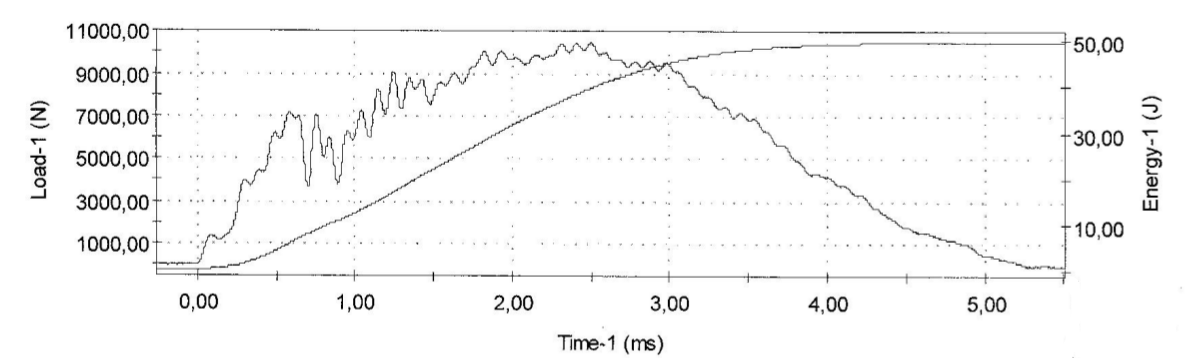
\includegraphics[width=\textwidth]{png/load-profile.png}}
\caption{Пример профиля нагрузки на обшивку крыла при испытаниях.}
\label{pic:loadprofile}
\end{figure}

Резюмируя, можно выделить следующие цели работы:
\begin{itemize}
\item предложить алгоритм построения параллельной версии сеточно"=характеристического метода в случае трёх пространственных переменных на неструктурированных сетках;
\item реализовать предложенный алгоритм в виде программного комплекса;
\item получить волновую картину в обшивке после низкоскоростного удара при
указаных выше допущениях.
\end{itemize}

\subsection*{Существующие работы на схожую тематику}
\addcontentsline{toc}{subsection}{Существующие работы на схожую тематику}

Для динамических задач механики деформируемого твердого тела необходимо использование численных методов, позволяющих получить полную волновую картину с высоким временным и пространственным разрешением с учётом влияния контактных границ. Так как определяющая система уравнений в частных производных относится к гиперболическому типу, одними из наиболее широко используемых вычислительных методов для её решения являются сеточно-характеристические методы, подробное описание и обзор которых можно найти в \cite{magomedov}. Главная особенность, присущая методу характеристик, -- нерегулярность разностной сетки -- оказалась серьёзным препятствием для обобщения этого метода на многомерный случай. Существенное продвижение здесь было получено в работах \cite{chushkin}, основанных на сочетании метода характеристик и конечно-разностных подходов.

В работе \cite{petrov_chelnokov} рассматриваются особенности протекания процессов деформирования в многослойных преградах конечной толщины, вызванных ударом абсолютно твёрдого сферического тела. Для моделирования поведения материала преграды использовались реологические модели линейно-упругой среды (закон Гука), упругопластической (модель Прандтля-Рейса с условиями пластичности Мизеса и Мизеса-Шлейхера, модель Маквелла), упруговязкопластической сред. Характерной особенностью работы является использование модели разрушения (модель Майнчена-Сака), а также использование различных подходов к перестроению сеток. Для численного решения использовался сеточно-характеристический метод, гибридная и гибридизованная разностные схемы. Минусами является использование структурированной (прямоугольной) сетки и только двух пространственных переменных.

В работе \cite{matyushev_petrov} проводилось численное исследование волновых и деформационных процессов в многослойных  средах. Как и в предыдущей работе, использовался численно-характеристический метод, а также гибридная и гибридизированная схемы. Особенностью является использование неструктурированных (треугольных) сеток, а также применение сеточно-характеристического шаблона на неструктурированных сетках (этот подход весьма необычен, так как использование шаблона предполагает наличие структурированной сетки). Моделировался удар деформируемым сферическим ударником по многослойной (5 – 20 слоев) преграде. Данная модель описывала пуленепробиваемый жилет и человеческое тело, защищённое им. Целью было найти оптимальные параметры среды для максимального поглощения воздействия ударника. К недостаткам работы можно отнести моделирование лишь по двум пространственным координатам.

В \cite{petrov_tormasov_holodov} рассматрены одномерные и двумерные нестационарные задачи о действии ударных и других нестационарных нагрузок на деформируемые твёрдые среды многослойной структуры, описаны возникающие волновые и откольные эффекты. Для описания поведения среды использованы модели линейно упругого и упругоидеальнопластического тела. На поверхностях раздела слоев рассматрены условия трёх типов: полного слипания, свободного скольжения, отслоения. В работе изучалось в основном влияние многослойных структур на амплитуду проходящей волны. На основании одномерных расчётов в слоистых средах был сделан вывод, что слоистые конструкции можно использовать для уменьшения амплитуды волн и для увеличения сжимающих напряжений вблизи лицевой поверхности, например, для увеличения силы сопротивления.

В \cite{golubev_kvasov_petrov} исследуются задачи распространения упругих волн, возникающих в результате землетрясения, в различных геологических средах: однородной, многослойной, градиентной, с трещиноватым пластом и карстовым образованием. Также проводится анализ воздействия упругих волн на поверхностные промышленные сооружения: здания и плотины. Проводится сравнение воздействия упругих волн на дневную поверхность для различных геологических сред. Качественно рассматривается влияние упругих волн на прочность поверхностных сооружений. В работе используется сеточно"=характеристический метод на треугольных сетках, контактные границы выделяются явно.

В \cite{agapov_belocerkovsky_petrov} сформулирована двумерная математическая модель механической реакции головы человека на ударные воздействия, описывающая пространственное распределение механических нагрузок на мозг (который в принципе является многослойной средой). Приведены некоторые результаты ее численного исследования с применением сеточно-характеристических методов на структурированных (прямоугольных) и неструктурированных (треугольных) сетках.

Работа \cite{petrov} посвящена численному исследованию волновых и откольных явлений, возникающих при импульсном нагружении двух- и четырехслойных упругопластических цилиндрических оболочек конечной толщины, подкрепленных с тыльной стороны ребрами жесткости. Используется динамическая система двумерных уравнений механики деформируемого тела и упруго идеально пластическая модель Прандтля-Рейсса. В работе показана возможность не только получать разрушенные зоны, но и отдельные трещины, зоны концентраций напряжений вблизи трещины и края откольной зоны, которая переходит в трещину, являющуюся самостоятельным источником нестационарных возмущений.

Автору не известны работы на схожую тематику, использующие сеточно-характеристический метод на неструктурированных сетках при трех пространственных переменных с явным выделением контактных границ.


\clearpage
\newpage
\section{Моделирование композиционных материалов}

\subsection{Строение и структура композитов}

\subsection{Волновые процессы в сплошных средах разной структуры}

\subsubsection{Однородная среда}

В однородной изотропной среде существует только два типа волн: поперечные и продольные (доказано Пуассоном, доказательство приведено в \cite{amenadze}\todo{стр. 249}). При этом продольные волны при распространении не генерируют поперечных и наоборот. Вывод формул для распространения плоской продольной, плоской поперечной и сферической продольной волн также приведен в \cite{amenadze}\todo{стр. 250}.

В случае точечного источника волн математическая ситуация несколько усложняется. Вывод приведен в \cite{aki_richards}\todo{стр. 73}. Подробно свойства P-волны, SH-волны и SV-волны рассмотрены в \cite{aki_richards}\todo{стр. 77}. В наших задачах нас интересует, по сути, только дальняя зона.

В однородной среде с какой-либо границей продольные и поперечные волны распространяются независимо лишь до того момента, пока фронт не пересечет границу. Тогда образуются так называемые отраженные и преломленные волны обоих типов, так как обычно системе граничных условий нельзя удовлетворить, введя отраженную волну какого-либо одного типа \cite{amenadze}\todo{стр. 250}. Подробная математика отражения и преломления плоских волн на плоских границах в однородных средах рассмотрена в \cite{aki_richards}\todo{стр. 121}. Выводы и диаграммы по отражению от свободной границы приведены в \cite{aki_richards} \todo{стр. 132, 136, 137 (P и SV), 140 (SH)}. Выводы и диаграммы по отражению и преломлению на жесткой границе двух твердых тел также рассмотрены в \cite{aki_richards}\todo{стр. 142, 143 (P и SV)}.


\subsubsection{Упругое полупространство}

Рассмотрим упругое полупространство и задачу о его свободных колебаниях. На границе полупространства - условие свободной границы, то есть действующая сила равна нулю. Вывод уравнений для получающихся волн приведен в \cite{aki_richards}\todo{стр. 253} и \cite{viktorov}\todo{стр. 5}. Эти волны впервые были исследованы Рэлеем. Стоит заметить, что решение ищется при условиях однородности по третьей оси координат (плоская деформация) и затухания с глубиной ("поверхностная" волна). Любая фиксированная точка изучаемого тела или породы при этом будет двигаться по эллипсу. Волны Рэлея имеют большое значение для геологических исследований, так как представляют наибольшую опасность при землетрясениях. Энергия, которую эти волны несут, сконцентрирована у поверхности и рассеивается по поверхности, ее рассеивание происходит медленнее, чем в тех волнах, где энергия рассеивается по объему возмущенной области. Свойства волн Рэлея также описаны в \cite{aki_richards}\todo{стр. 156}, \cite{tischenko}. Заметим, что в \cite{aki_richards} произведен вывод формул для волн Релея с точки зрения отражения неоднородной по горизонтальной медленности P- и SV- волн.

В 1904 году Лэмб дал точное решение задачи, в которой источник действовал как импульс, приложенный к свободной границе твердого полупространства по нормали к ней \cite{lamb}. Однако теперь термин "задача Лэмба" относят к более общему случаю произвольного источника в среде с одной границей.

Математика отражения сферической волны от плоской свободной границы (цилиндрическая симметрия) подробно рассмотрена в \cite{aki_richards}\todo{стр. 206, краткие итоги анализа уравнений — стр. 211, свойства цилиндрической волны Рэлея — стр. 214}.

О способах генерации волн Рэлея написано в \cite{viktorov}\todo{стр. 12}.


\subsubsection{Два упругих полупространства}

При наличии двух упругих полупространств с различными свойствами, как показано в \cite{aki_richards}, стр. 156, по аналогии с волнами Рэлея возникают волны Стоунли. Такие волны всегда могут существовать на границе жидкости и твердого тела, но, при определенном соотношении свойств материалов, могут появляться и на границе двух твердых тел. Волны Стоунли, аналогично рэлеевским, не обладают дисперсией.

Горизонтальная плоская граница создает связь плоских волн P- и SV-, а волны SH- распространяются независимо от них \cite{aki_richards}, стр. 207).

Математика отражения и преломления сферической волны на плоской границе подробно рассмотрена в \cite{aki_richards}, стр. 192. Когда сферическая волна взаимодействует с плоской границей между двумя различными полупространствами, образующуюся систему волн можно естественно разделить на три основных группы: 1) волны, естественно отраженные от границы или преломленные на ней; 2) головные волны; 3) волны типа Рэлея и Стоунли (\cite{aki_richards}, стр. 186). Заметим, что головные волны — это не прямые волны, которые появляются на приемнике при распространении непосредственно от источника, а отдельный тип волн с той же скоростью распространения, но с другими свойствами (\cite{aki_richards}, стр. 203).


\subsubsection{Один слой и упругое полупространство}

Рассмотрим упругий слой постоянной толщины, лежащий на упругом полупространстве из другого материала (с большей скоростью распространения поперечных волн). Ищем поперечную волну, которая будет распространяться вдоль границы раздела как в слое, так и в полупространстве. Подробный вывод уравнений - \cite{amenadze}, стр. 256. Такие волны называется волнами Лява. Аналогично рэлеевским волнам, энергия волн Лява концентрируется вблизи границы раздела двух сред, поэтому может наблюдаться на значительном удалении от эпицентра возмущения. В отличие от релеевских волн, волны Лява имеют дисперсию (фазовая скорость зависит от частоты).


\subsubsection{Один слой}

Случай тонкой пластинки рассмотрен в \cite{amenadze}, стр. 259. 

Волны Лэмба (волны в пластинке конечной толщины) подробно рассмотрены в \cite{viktorov}, стр. 78 (математика), стр. 87 (свойства), стр. 96 (возбуждение). На стр. 107 приведено сравнение волн Лэмба с волнами Рэлея. Делается вывод, что при стремлении толщины пластинки к бесконечности волны Лэмба переходят в волну Рэлея. При конечной толщине можно говорить о квазирэлеевской волне. Она распространяется вдоль поверхности, к которой прилагалось начальное возмущение, и на некотором расстоянии, зависящем от толщины пластинки, переходит на противоположную поверхность. 


\subsubsection{Слойка}

Случай жидкого слоя в твердом слоистом полупространстве рассмотрен в \cite{aki_richards}, стр. 266.


\subsubsection{Объемные волны}

Продольные волны (они же объемные волны) — волны, в которых направление распространения совпадает с мнговенной скоростью частиц. Они наблюдаются при возмущении в однородной среде (или при достаточной удаленности от границ).

Поперечные волны (они же сдвиговые волны) — волны, в которых направление распространения первендикулярно мнговенной скорости частиц. Они также наблюдаются в однородной среде. Условное разделение поперечных волн на SH и SV происходит при появлении плоской границы. SH-волнами называют поперечные волны, мгновенная скорость частиц в которой параллельна этой плоской границе. Они появляются только в трехмерном случае, в двухмерном случае (а также квазидвухмерном или цилиндрически симметричном) таких волн нет. Соответственно, SV-волны — это любые другие.

Продольные и поперечные волны могут иметь различную форму фронта. В аналитических исследованиях чаще всего говорят о плоском и сферическом фронтах, как самых простых для математического анализа. В задаче о точечном источнике обычно фигурирует сферическая форма фронта.

Продольные и сдвиговые волны не зависят друг от друга в однородном пространстве. При наличии границ появляется связь между P- и SV- волнами, так как при отражении и преломлении они друг друга порождают. SH-волны распространяются независимо от P- и SV-.

Других волн в однородном пространстве не наблюдается, что доказано Пуассоном.


\subsubsection{Поверхностные волны}
Волны Рэлея появляются в упругом полупространстве при наличии свободной границы. В случае более сложной геометрии говорить о наличии волн Рэлея не вполне корректно, однако если полупространство является однородным на расстоянии, большем длины волны (достаточно широкий верхний слой), то данный термин вполне применим, а сравнение с аналитическим выводом правомерно. Волны Рэлея появляются как в двухмерной постановке, так и в трехмерной. Достаточно просто они генерируются при обычной постановке задачи Лэмба (удар по свободной поверхности) и при отражении сферического фронта продольной волны. В трехмерной постановке фронт волны Рэлея является цилиндрическим. В волне Рэлея частицы движутся по эллипсу.

Волны Стоунли полностью аналогичны волнам Рэлея, но появляются при наличии плоской границы между двумя упругими полупространствами. Аналогично, об их наличии мы можем говорить только в том случае, если толщина слоя достаточно велика, как в двухмерном, так и в трехмерном случае.

Волны Лява наблюдаются только в трехмерном случае и возникают только на границе между упругим полупространством и лежащем на нём слое с верхней свободной границей. Движение частиц параллельно плоскости границы и перепендикулярно направлению распространения. Эти волны легко отличить от волн Стоунли и Рэлея, так как мгновенное направление скоростей частиц в них перпендикулярны аналогичным у последних.

Головные волны распространяются к приемнику от источника по пути, включающему скольжение вдоль границы со скоростью объемной волны.

Волны Лэмба наблюдаются в случае пластинки конечной толщины. Они бывают симметричными и антисимметричными, причем количество их конечно и зависит от толщины пластинки. При достаточной толщине интерференция волн Лэмба нулевого порядка дает квазирэлеевскую волну, которая на некотором расстоянии от точки начального возмущения переходит на противоположную поверхность, а при бесконечной толщине стремится к рэлеевской. 

Других волн в случае рассмотренных геометрий (полупространство, два полупространства, слой на полупространстве, один слой) не наблюдается.


\subsubsection{Постановка задачи для многослойной конструкции}

Можно сделать вывод, что при рассмотрении многослойной конструкции с достаточно широкими (в сравнении с длинами волн) слоями, мы можем говорить о наличии волн Рэлея в верхнем слое и волн Стоунли в остальных слоях. При асимметричном начальном возмущении мы можем получить волну, которую будет достаточно корректно назвать волной Лява. Обычно для ее получения в численном расчете задается достаточно сложная геометрия начального импульса, но она должна формироваться при любом неоднородном и несимметричном начальном возмущении в постановке, аналогичной постановке задачи Лэмба.

Волны Лэмба также могут нас интересовать: в случае однородной пластинки мы можем сравнить с аналитикой расстояние, на котором происходит переход квазирэлеевской волны (интерференции волн Лэмба нулевого порядка) на противоположную поверхность. Возможно, аналогичный эффект перехода будет наблюдаться и при несвободной нижней границе, т.е. в многослойной конструкции.

Также заметим, что для получения поверхностных волн необходим достаточно долгий расчет: они формируются не сразу. Однако со временем они не только демонстрируют характерные и легко отличимые эллиптические фронты, но и выделяются по масштабу, так как затухают гораздо медленнее объемных волн. 

Для сравнения нашего метода с аналитикой лучше брать самые простые постановки. Упругое полупространство с плоской свободной границей, два упругих полупространства с полным слипанием между ними, однородную плоскую пластинку. Плоский (под различными углами) или сферический фронты начальных возмущений. Количественно сравнивать с аналитикой при этом можно амплитуды отраженной и преломленной волны (плоский фронт под различными углами), скорость и амплитуду волн Рэлея и Стоунли (сферический фронт), расстояние перехода и амплитуду квазирэлеевской волны в случае однородной пластинки (интерференция волн Лэмба). Аналитические выражения достаточно взять из \cite{aki_richards} и \cite{viktorov}. Учитывая сложность математики, приведенной для простых случаев, многослойную постановку в аналитикой сравнивать в ближайшее время не получится. Однако при достаточной ширине слоев (больше длин поверхностных волн) мы можем говорить об аналогии полученных волн с известными нам волнами Рэлея и Стоунли.


\subsection{Методы и подходы к моделированию композитов}


\clearpage
\newpage
\section{Математическая модель}

\subsection{Уравнения механики твёрдого тела}
Для математического моделирования волновых процессов в деформируемом твёрдом
теле используется система динамических уравнений \cite{novatsky,sedov} в виде
\begin{eqnarray}
\label{initial_equations}
\rho\dot{v}_i=\nabla_j\sigma_{ij}+f_i & \textrm{(уравнения движения)}\nonumber\\
\sigma_{ij}=q_{ijkl}\dot{\varepsilon}_{kl}+F_{ij} & \textrm{(реологические
соотношения).}
\end{eqnarray}

Здесь $\rho$ – плотность среды, $v_i$ – компоненты скорости смещения,
$\sigma_{ij}$, $\varepsilon_{ij}$ -- компоненты тензоров напряжений и деформаций,
$\nabla_j$ – ковариантная производная по $j$-й координате, $f_i$ – массовые
силы, действующие на единицу объёма, $F_{ij}$ -- правая часть, используемая, например, для описания диссипации в моделях с учётом вязкости.

В случае малых деформаций тензор скоростей деформаций $e_{ij}=\dot{\varepsilon}_{ij}$ 
выражается через компоненты скорости смещения линейным образом:
\begin{equation}
e_{ij}=\frac{1}{2}(\nabla_j v_i+\nabla_i v_j).
\end{equation}

Вид компонент тензора 4-го порядка $q_{ijkl}$ и правой части $F_{ij}$ определяется реологией среды.

Для замыкания системы уравнений \ref{initial_equations} её необходимо дополнить
уравнением состояния, определяющим зависимость плотности от напряжений:
$$\rho=\rho_0e^{\frac{p}{K}},$$
где $p=-\frac{1}{3}\sum\sigma_{kk}$ -- давление, $K=\lambda+\frac{2}{3}\mu$ --
коэффициент всестороннего сжатия, $\lambda$ и $\mu$ -- параметры Ламе.

Параметры Ламе зависят от материала и связаны с модулем продольной упругости и коэффициентом Пуассона следующим образом:
\begin{eqnarray}
\label{lame_parameters}
\lambda=\frac{E\nu}{(1+\nu)(1-2\nu)}
\nonumber\\
\mu=G=\frac{E}{2(1+\nu)}
\end{eqnarray}
Здесь $E$ -- модуль продольной упругости, $\nu$ -- коэффициент Пуассона, $G$ -- модуль сдвига.

В простейшем случае линейной упругости $q_{ijkl}=\lambda\delta_{ij}\delta_{kl}+\mu(\delta_{ik}\delta_{jl}+\delta_{il}\delta_{jk})$ и $F_{ij}=0$. Тогда в приближении малых деформаций и в отсутствии внешних сил в трехмерном пространстве и декартовых координатах уравнения \ref{initial_equations} принимают вид

\begin{eqnarray}
\label{simple_equations}
\frac{\partial{v_x}}{\partial{t}}=\frac{1}{\rho}(\frac{\partial{\sigma_{xx}}}{\partial{x}}+\frac{\partial{\sigma_{xy}}}{\partial{y}}+\frac{\partial{\sigma_{xz}}}{\partial{z}})
\nonumber\\
\frac{\partial{v_y}}{\partial{t}}=\frac{1}{\rho}(\frac{\partial{\sigma_{xy}}}{\partial{x}}+\frac{\partial{\sigma_{yy}}}{\partial{y}}+\frac{\partial{\sigma_{yz}}}{\partial{z}})
\nonumber\\
\frac{\partial{v_z}}{\partial{t}}=\frac{1}{\rho}(\frac{\partial{\sigma_{xz}}}{\partial{x}}+\frac{\partial{\sigma_{yz}}}{\partial{y}}+\frac{\partial{\sigma_{zz}}}{\partial{z}})
\nonumber\\
\frac{\partial{\sigma_{xx}}}{\partial{t}}=(\lambda+2\mu)\frac{\partial{v_x}}{\partial{x}}+\lambda\frac{\partial{v_y}}{\partial{y}}+\lambda\frac{\partial{v_z}}{\partial{z}}
\nonumber\\
\frac{\partial{\sigma_{xy}}}{\partial{t}}=\mu(\frac{\partial{v_x}}{\partial{y}}+\frac{\partial{v_y}}{\partial{x}})
\nonumber\\
\frac{\partial{\sigma_{xz}}}{\partial{t}}=\mu(\frac{\partial{v_x}}{\partial{z}}+\frac{\partial{v_z}}{\partial{x}})
\nonumber\\
\frac{\partial{\sigma_{yy}}}{\partial{t}}=\lambda\frac{\partial{v_x}}{\partial{x}}+(\lambda+2\mu)\frac{\partial{v_y}}{\partial{y}}+\lambda\frac{\partial{v_z}}{\partial{z}}
\nonumber\\
\frac{\partial{\sigma_{yz}}}{\partial{t}}=\mu(\frac{\partial{v_z}}{\partial{y}}+\frac{\partial{v_y}}{\partial{z}})
\nonumber\\
\frac{\partial{\sigma_{zz}}}{\partial{t}}=\lambda\frac{\partial{v_x}}{\partial{x}}+\lambda\frac{\partial{v_y}}{\partial{y}}+(\lambda+2\mu)\frac{\partial{v_z}}{\partial{z}}
\end{eqnarray}

Очевидно, что уравнения \ref{simple_equations} можно переписать в матричной форме:
\begin{equation}
\label{simple_matrix_equation}
\frac{\partial\vec{u}}{\partial{t}}+\mathbf{A}_x\frac{\partial\vec{u}}{\partial{x}}+
\mathbf{A}_y\frac{\partial\vec{u}}{\partial{y}}+
\mathbf{A}_z\frac{\partial\vec{u}}{\partial{z}}=0.
\end{equation}
Здесь
$\vec{u}=\{v_x,v_y,v_z,\sigma_{xx},\sigma_{yy},\sigma_{zz},\sigma_{xy},\sigma_{xz},\sigma_{yz}\}^T$
-- вектор искомых функций, $x,y,z$ --  независимые пространственные переменные, $t$ -- время.

Аналогично можно записать более общую систему \ref{initial_equations} в виде:
\begin{equation}
\label{matrix_equation}
\frac{\partial\vec{u}}{\partial{t}}+\mathbf{A}_x\frac{\partial\vec{u}}{\partial{x}}+
\mathbf{A}_y\frac{\partial\vec{u}}{\partial{y}}+
\mathbf{A}_z\frac{\partial\vec{u}}{\partial{z}}=\vec{f}.
\end{equation}
Здесь $\vec{f}$ -- вектор правых частей, размерность которого равна размерности исходной системы, а выражения для компонентов зависят от реологии среды. Точный вид матриц $\mathbf{A}_x$, $\mathbf{A}_y$, $\mathbf{A}_z$ также зависит от реологии среды.

\clearpage
\newpage

\subsection{Приближение линейно упругого тела}

\subsubsection{Реологические соотношения для линейно упругого тела}

Для линейно упругого тела тензор $q_{ijkl}$ и правая часть $F_{ij}$ в \ref{initial_equations} принимают следующий вид:
\begin{eqnarray}
\label{tensor_qijkl_elastic}
q_{ijkl}=\lambda\delta_{ij}\delta_{kl}+\mu(\delta_{ik}\delta_{jl}+\delta_{il}
\delta_{jk}),\nonumber\\
F_{ij}=0.
\end{eqnarray}
В этом соотношении $\lambda$ и $\mu$ -- параметры Ламе, $\delta_{ij}$ -- символ Кронекера.

\subsubsection{Матричная форма уравнений в случае линейно упругого тела}

Для линейно упругого тела матрицы $\mathbf{A}_x$, $\mathbf{A}_y$, $\mathbf{A}_z$ в \ref{matrix_equation} принимают следующий вид.

\begin{displaymath}
\mathbf{A}_x =
\left( \begin{array}{cccccccccccc}
0 & 0 & 0 & -\frac 1 \rho & 0 & 0 & 0 & 0 & 0 \\ 
0 & 0 & 0 & 0 & -\frac 1 \rho & 0 & 0 & 0 & 0 \\ 
0 & 0 & 0 & 0 & 0 & -\frac 1 \rho & 0 & 0 & 0 \\ 
-(\lambda+2\mu) & 0 & 0 & 0 & 0 & 0 & 0 & 0 & 0 \\ 
0 & -\mu & 0 & 0 & 0 & 0 & 0 & 0 & 0 \\ 
0 & 0 & -\mu & 0 & 0 & 0 & 0 & 0 & 0 \\ 
-\lambda & 0 & 0 & 0 & 0 & 0 & 0 & 0 & 0 \\ 
0 & 0 & 0 & 0 & 0 & 0 & 0 & 0 & 0 \\ 
-\lambda & 0 & 0 & 0 & 0 & 0 & 0 & 0 & 0  
\end{array} \right),
\end{displaymath} 
\begin{displaymath}
\mathbf{A}_y =
\left( \begin{array}{cccccccccccc}
0 & 0 & 0 & 0 & -\frac 1 \rho & 0 & 0 & 0 & 0 \\ 
0 & 0 & 0 & 0 & 0 & 0 & -\frac 1 \rho & 0 & 0 \\ 
0 & 0 & 0 & 0 & 0 & 0 & 0 & -\frac 1 \rho & 0 \\ 
0 & -\lambda & 0 & 0 & 0 & 0 & 0 & 0 & 0 \\ 
-\mu & 0 & 0 & 0 & 0 & 0 & 0 & 0 & 0 \\ 
0 & 0 & 0 & 0 & 0 & 0 & 0 & 0 & 0 \\ 
0 & -(\lambda+2\mu) & 0 & 0 & 0 & 0 & 0 & 0 & 0 \\ 
0 & 0 & -\mu & 0 & 0 & 0 & 0 & 0 & 0 \\ 
0 & -\lambda & 0 & 0 & 0 & 0 & 0 & 0 & 0  
\end{array} \right),
\end{displaymath}
\begin{displaymath}
\mathbf{A}_z =
\left( \begin{array}{cccccccccccc}
0 & 0 & 0 & 0 & 0 & -\frac 1 \rho & 0 & 0 & 0 \\ 
0 & 0 & 0 & 0 & 0 & 0 & 0 & -\frac 1 \rho & 0 \\ 
0 & 0 & 0 & 0 & 0 & 0 & 0 & 0 & -\frac 1 \rho \\ 
0 & 0 & -\lambda & 0 & 0 & 0 & 0 & 0 & 0 \\ 
0 & 0 & 0 & 0 & 0 & 0 & 0 & 0 & 0 \\ 
-\mu & 0 & 0 & 0 & 0 & 0 & 0 & 0 & 0 \\ 
0 & 0 & -\lambda & 0 & 0 & 0 & 0 & 0 & 0 \\ 
0 & -\mu & 0 & 0 & 0 & 0 & 0 & 0 & 0 \\ 
0 & 0 & -(\lambda+2\mu) & 0 & 0 & 0 & 0 & 0 & 0  
\end{array} \right).
\end{displaymath}

\clearpage
\newpage

\subsection{Приближение упруго-пластического тела}

\subsubsection{Реологические соотношения для упруго-пластического тела}

Для упруго-пластического тела тензор $q_{ijkl}$ и правая часть $F_{ij}$ в \ref{initial_equations} имеют более сложный вид:
\begin{eqnarray}
\label{tensor_qijkl_plastic}
q_{ijkl}=\lambda\delta_{ij}\delta_{kl}+\mu(\delta_{ik}\delta_{jl}+\delta_{il}\delta_{jk})-\frac{I\mu\sigma_{ij}\sigma_{kl}}{K^2},
\nonumber\\
F_{ij}=0.
\end{eqnarray}
В этом соотношении $\lambda$ и $\mu$ -- параметры Ламе, $K$ -- предел текучести на сдвиг, $\sigma_{ij}$ -- компоненты тензора напряжений, $\delta_{ij}$ -- символ Кронекера, $I$ -- параметр модели, который определяется следующим образом:
\todo{Имени кого модель? И точный вид S для 3D?}
\begin{equation}
\label{I_parameter_plastic}
I=\begin{cases}
0, & \text{если $S = \sigma_{xx}^2+\sigma_{yy}^2+\sigma_{zz}^2+2\sigma_{xy}^2 < 2K^2$}\\
1, & \text{если $S >= 2K^2$}.
\end{cases}
\end{equation}

\subsubsection{Матричная форма уравнений в случае упруго-пластического тела}

Для линейно упругого тела матрицы $\mathbf{A}_x$, $\mathbf{A}_y$, $\mathbf{A}_z$ в \ref{matrix_equation} имеют существенно более сложный вид, так как компоненты тензора $q_{ijkl}$ зависят от компонентов тензора $\sigma$. Значения $\sigma_{ij}$ в общем случае различны в каждой точке пространства в каждый момент времени. Это приводит к тому, что невозможно упростить вид матриц аналитически и получить их покомпонентную запись в терминах $\lambda, \mu, \rho$, как это было сделано для линейно упругого тела. Значения ненулевых элементов каждой матрицы необходимо вычислять в каждой точке пространства в каждый момент времени в соответствии с \ref{tensor_qijkl_plastic} и \ref{I_parameter_plastic}, используя текущие значения $\sigma_{ij}$ в данной точке.

\begin{displaymath}
\mathbf{A}_x =
\left( \begin{array}{cccccccccccc}
0 & 0 & 0 & -\frac 1 \rho & 0 & 0 & 0 & 0 & 0 \\ 
0 & 0 & 0 & 0 & -\frac 1 \rho & 0 & 0 & 0 & 0 \\ 
0 & 0 & 0 & 0 & 0 & -\frac 1 \rho & 0 & 0 & 0 \\ 
-q_{1111} & -\frac{q_{1112}+q_{1121}}{2} & -\frac{q_{1113}+q_{1131}}{2} & 0 & 0 & 0 & 0 & 0 & 0 \\ 
-q_{1211} & -\frac{q_{1212}+q_{1221}}{2} & -\frac{q_{1213}+q_{1231}}{2} & 0 & 0 & 0 & 0 & 0 & 0 \\ 
-q_{1311} & -\frac{q_{1312}+q_{1321}}{2} & -\frac{q_{1313}+q_{1331}}{2} & 0 & 0 & 0 & 0 & 0 & 0 \\ 
-q_{2211} & -\frac{q_{2212}+q_{2221}}{2} & -\frac{q_{2213}+q_{2231}}{2} & 0 & 0 & 0 & 0 & 0 & 0 \\ 
-q_{2311} & -\frac{q_{2312}+q_{2321}}{2} & -\frac{q_{2313}+q_{2331}}{2} & 0 & 0 & 0 & 0 & 0 & 0 \\ 
-q_{3311} & -\frac{q_{3312}+q_{3321}}{2} & -\frac{q_{3313}+q_{3331}}{2} & 0 & 0 & 0 & 0 & 0 & 0  
\end{array} \right),
\end{displaymath} 
\begin{displaymath}
\mathbf{A}_y =
\left( \begin{array}{cccccccccccc}
0 & 0 & 0 & 0 & -\frac 1 \rho & 0 & 0 & 0 & 0 \\ 
0 & 0 & 0 & 0 & 0 & 0 & -\frac 1 \rho & 0 & 0 \\ 
0 & 0 & 0 & 0 & 0 & 0 & 0 & -\frac 1 \rho & 0 \\ 
-\frac{q_{1112}+q_{1121}}{2} & -q_{1122} & -\frac{q_{1123}+q_{1132}}{2} & 0 & 0 & 0 & 0 & 0 & 0 \\ 
-\frac{q_{1212}+q_{1221}}{2} & -q_{1222} & -\frac{q_{1223}+q_{1232}}{2} & 0 & 0 & 0 & 0 & 0 & 0 \\ 
-\frac{q_{1312}+q_{1321}}{2} & -q_{1322} & -\frac{q_{1323}+q_{1332}}{2} & 0 & 0 & 0 & 0 & 0 & 0 \\ 
-\frac{q_{2212}+q_{2221}}{2} & -q_{2222} & -\frac{q_{2223}+q_{2232}}{2} & 0 & 0 & 0 & 0 & 0 & 0 \\ 
-\frac{q_{2312}+q_{2321}}{2} & -q_{2322} & -\frac{q_{2323}+q_{2332}}{2} & 0 & 0 & 0 & 0 & 0 & 0 \\ 
-\frac{q_{3312}+q_{3321}}{2} & -q_{3322} & -\frac{q_{3323}+q_{3332}}{2} & 0 & 0 & 0 & 0 & 0 & 0  
\end{array} \right),
\end{displaymath}
\begin{displaymath}
\mathbf{A}_z =
\left( \begin{array}{cccccccccccc}
0 & 0 & 0 & 0 & 0 & -\frac 1 \rho & 0 & 0 & 0 \\ 
0 & 0 & 0 & 0 & 0 & 0 & 0 & -\frac 1 \rho & 0 \\ 
0 & 0 & 0 & 0 & 0 & 0 & 0 & 0 & -\frac 1 \rho \\ 
-\frac{q_{1113}+q_{1131}}{2} & -\frac{q_{1123}+q_{1132}}{2} & -q_{1133} & 0 & 0 & 0 & 0 & 0 & 0 \\ 
-\frac{q_{1213}+q_{1231}}{2} & -\frac{q_{1223}+q_{1232}}{2} & -q_{1233} & 0 & 0 & 0 & 0 & 0 & 0 \\ 
-\frac{q_{1313}+q_{1331}}{2} & -\frac{q_{1323}+q_{1332}}{2} & -q_{1333} & 0 & 0 & 0 & 0 & 0 & 0 \\ 
-\frac{q_{2213}+q_{2231}}{2} & -\frac{q_{2223}+q_{2232}}{2} & -q_{2233} & 0 & 0 & 0 & 0 & 0 & 0 \\ 
-\frac{q_{2313}+q_{2331}}{2} & -\frac{q_{2323}+q_{2332}}{2} & -q_{2333} & 0 & 0 & 0 & 0 & 0 & 0 \\ 
-\frac{q_{3313}+q_{3331}}{2} & -\frac{q_{3323}+q_{3332}}{2} & -q_{3333} & 0 & 0 & 0 & 0 & 0 & 0  
\end{array} \right).
\end{displaymath}

\clearpage
\newpage

\subsection{Преобразование уравнений при смене базиса}

\todo{Вывод. Вид матриц. Анализ матриц. Неортогональный базис. Исследование последствий для шага по времени.}

\clearpage
\newpage
\section{Численный метод}

Перед тем, как перейти к исследованию полной задачи \ref{matrix_equation} в трёхмерной постановке, рассмотрим одномерное уравнение вида
\begin{equation}
\frac{\partial\vec{u}}{\partial{t}}+\mathbf{A}\frac{\partial\vec{u}}{\partial{x}}=0.
\label{advection_equation}
\end{equation}

\subsection{Решение одномерной задачи}

\subsubsection{Гиперболические свойства системы уравнений}
\label{sec:hyperbolic_features}

Если матрица $\mathbf{A}$ имеет полный набор вещественных собственных значений, 
то такое уравнение называется гиперболическим, и его решения соответствуют 
процессам, которые носят волновой характер. Спектральное исследование матриц $\mathbf{A}_x$, $\mathbf{A}_y$, $\mathbf{A}_z$ проведено в \cite{chelnokov}, где показано, что для них существует полный набор собственных значений и собственных векторов.

В этом случае для любой из матриц $\mathbf{A}_x$, $\mathbf{A}_y$, $\mathbf{A}_z$ существует разложение:
\begin{equation}
\mathbf{A}=\mathbf\Omega^{-1}\mathbf\Lambda\mathbf\Omega,
\end{equation}
где $\mathbf\Omega$ -- матрица, строки которой $\vec\omega_i^T$ являются собственными для матрицы $\mathbf A$ и
удовлетворяют соотношениям
\begin{equation}
\vec\omega_i^T\mathbf A=\lambda_i\vec\omega_i^T
\end{equation}
или, что то же самое, транспонированные строки $\mathbf\Omega$ являются собственными векторами для матрицы $\mathbf A^T$
\begin{equation}
\mathbf A^T\vec\omega_i=\lambda_i\vec\omega_i.
\end{equation}
Здесь $\mathbf\Lambda=diag\{\lambda_i\}$ -- диагональная матрица соответствующих собственных значений.

Домножив уравнение \ref{advection_equation} слева на $\mathbf\Omega$, получаем уравнение
\begin{equation}
\frac{\partial{\mathbf\Omega{\vec u}}}{\partial t}+
\Lambda\frac{\partial{\mathbf\Omega{\vec u}}}{\partial x}=0,
\end{equation}
которое после перехода к инвариантам Римана ${\vec v}=\mathbf\Omega{\vec u}$ приобретает вид
\begin{equation}
\frac{\partial{\vec v}}{\partial t}+
\Lambda\frac{\partial{\vec v}}{\partial x}=0
\end{equation}
и тем самым распадается на $n$ одномерных уравнений вида
\begin{equation}
\frac{\partial{v_i}}{\partial t}+\lambda_i\frac{\partial{v_i}}{\partial x}=0.
\label{advection_equation_splitted}
\end{equation}
Таким образом, решение уравнения \ref{advection_equation} представляется в виде
суммы плоских волн, движущихся со скоростями $\lambda_i$.


\subsubsection{Сеточно-характеристический метод}
\label{sec:gcm_method_idea}

После перехода к инвариантам Римана получено 9 независимых уравнений переноса вида \ref{advection_equation_splitted}. Рассмотрим уравнение такого вида подробнее. Вдоль характеристических кривых $\Gamma$, таких что
\begin{equation}
\label{characteristics}
\frac{dx}{dt} = \lambda,
\end{equation}
уравнение \ref{advection_equation_splitted} принимает вид 
\begin{equation}
\label{characteristic_equation}
\frac{dv_i}{dt} = 0.
\end{equation}
Таким образом, значения инвариантов Римана переносятся с временного слоя $n$ на временной слой $n+1$ вдоль характеристических кривых $\Gamma$. При этом очевидно, что значения $\lambda_i$ будут разные в зависимости от вида матрицы $\mathbf A$, который определяется используемыми реологическими соотношениями.

\begin{figure}[h]
\center{\includegraphics[width=0.5\textwidth]{eps/gcm-idea.eps}}
\caption{Принципиальная схема сеточно-характеристического метода.}
\end{figure}

Алгоритм поиска значений исходных переменных $\vec u$ в некоторой точке $x_m^{n+1}$ на новом временном слое состоит в следующем. Сначала для матрицы $\mathbf A$ необходимо найти собственные числа $\lambda_i$, которые определяют наклон характеристик \ref{characteristics}, выпущенных из точки $x_m^{n+1}$. После этого для каждой характеристики $\Gamma_i$ можно определить точку $x_{i*}^n$ пересечения с временным слоем $n$.

В точке $x_{i*}^n$ тем или иным способом определяются значения переменных $\vec u_{i*}^n$. Способы реконструкции могут быть различными, в данной работе используется интерполяция по сеточному шаблону на предыдущем временном слое (подробнее см.ниже). По найденным значениям $\vec u_{i*}^n$ вычисляется $i$-ый инвариант Римана $v_{i*}^n$ в точке $x_{i*}^n$. Значение инварианта вдоль $\Gamma_i$ будет перенесено в точку $x_m^{n+1}$ на новом временном слое:
\begin{equation}
v_{im}^{n+1} = v_{i*}^n.
\end{equation}

После того, как в точке $x_m^{n+1}$ описанным образом найдены все 9 инвариантов Римана, можно найти в ней исходные переменные $\vec u$. Так как по определению ${\vec v}=\mathbf\Omega{\vec u}$, то
\begin{equation}
{\vec u}_m^{n+1}=\mathbf\Omega^{-1}{\vec v}_*^n,
\end{equation}
где ${\vec v}_*^n$ -- вектор, составленный из значений $v_{i*}^n$, подсчитанных в соответствующих точках на временном слое $n$. Как описано выше, точки, из которых берутся разные компоненты этого вектора, различны.


\subsubsection{Разностные схемы для структурированных сеток}

При использовании структурированных прямоугольных сеток описанный выше алгоритм для уравнения \ref{advection_equation} после выполнения математических преобразований приводит к известным разностным схемам.

\paragraph{Схема Куранта-Изаксона-Рис.} Данная схема строится на трёхточечном сеточном шаблоне $(m-1, m, m+1)$ и позволяет явно выразить значение $u_m^{n+1}$ на новом временном слое:

\begin{equation}
	\label{CIR scheme}
	u^{n+1}_m = u^n_m - \frac{\tau}{h} \Omega^{-1} \Lambda^+ \Omega (u^n_{m+1} - u^n_m) 
	- \frac{\tau}{h} \Omega^{-1} \Lambda^- \Omega (u^n_m – u^n_{m-1}) .
\end{equation}

Схема обладает первым порядком аппроксимации по времени и пространству $O(h, \tau)$, является монотонной и обеспечивает минимальное размытие волнового фронта среди всех схем первого порядка.

\paragraph{Схема Лакса-Вендрофа.} Данная схема является единственной схемой второго порядка точности на шаблоне $(m-1, m, m+1)$. Схема записывается в виде:

\begin{equation}
	\label{LW scheme}
	u^{n+1}_m = u^n_m - \frac{\tau}{2h} A (u^n_{m+1} - u^n_{m-1})
	 - \frac{\tau^2}{2h^2} A^2 (u^n_{m+1} - 2u^n_m + u^n_{m-1}) .
\end{equation}

Так как схема имеет второй порядок аппроксимации, она обеспечивает более точное воспроизведение формы волнового фронта по сравнению со схемами первого порядка. Однако, она не является монотонной, что приводит к появлению нефизичных численных осцилляций на разрывах точного решения.


\paragraph{Гибридная схема.} Для сочетания достоинств и преодоления недостатков обоих схем используется гибридная схема, являющаяся их линейной комбинацией. Гибридная схема имеет следующий общий вид:

\begin{align}
\label{hybrid scheme}
u^{n+1}_m &= u^n_m - \frac{\tau}{2h} A (u^n_{m+1} - u^n_{m-1}) + \nonumber\\
	 &+ \frac{1}{2} ((1-a) \frac{\tau}{h} \Omega^{-1} |\Lambda| \Omega + a \frac{\tau^2}{h^2} A^2 ) (u^n_{m+1} - 2u^n_m + u^n_{m-1}).
\end{align}

При $a = 0$ схема переходит в схему Куранта-Изаксона-Рис и имеет первый порядок аппроксимации. При $a = 1$ схема переходит в схему Лакса-Вендрофа и имеет второй порядок аппроксимации. Если параметр $a$ выбирается фиксированно из диапазона $0 < a < 1$, то схема называется гибридизованной, а полученной численное решение является некоторым усреднением решений первого и второго порядка. Схема называется гибридной, если значение $a$ выбирается независимо в каждой точке сетки на каждом временном шаге в зависимости от локальных свойств численного решения.

В данной работе использовался критерий переключения опорных схем, предложенный Р.П. Федоренко и основанный на локальной гладкости решения:

\begin{equation}
	\label{Fedorenko criterium}
	\frac{(u^n_{m+1} - 2u^n_m + u^n_{m-1})}{2} \le K \frac{(u^n_{m+1} – u^n_{m-1})}{2} .
\end{equation}

Параметр переключения $K$ подбирается в зависимости от задачи. В данной работе использовалось значение $K = 0.5$. Если условие \ref{Fedorenko criterium} не выполнено, решение считается разрывным и параметр $a$ принимает в данной точке значение $0$. Если условие \ref{Fedorenko criterium} выполнено -- параметр принимает значение $1$.

В результате применения такого подхода гладкие участки решения считаются схемой второго порядка, а разрывные -- схемой первого порядка. Гибридная схема позволяет получить минимальное размытие точного решения, но при этом избежать нефизичных осцилляций на разрывных решениях. На рис. \ref{pic:hybrid-scheme-testing} приведение сравнение схемы первого порядка, второго порядка, гибридной схемы и точного решения. Приведено решение задачи о распространении прямоугольного импульса нагрузки в однородной среде. Ширина импульса составляет 40 узлов сетки, к моменту, изображённому на рисунке, импульс прошел 200 узлов сетки от первоначального положения.

\begin{figure}[h]
\centerline{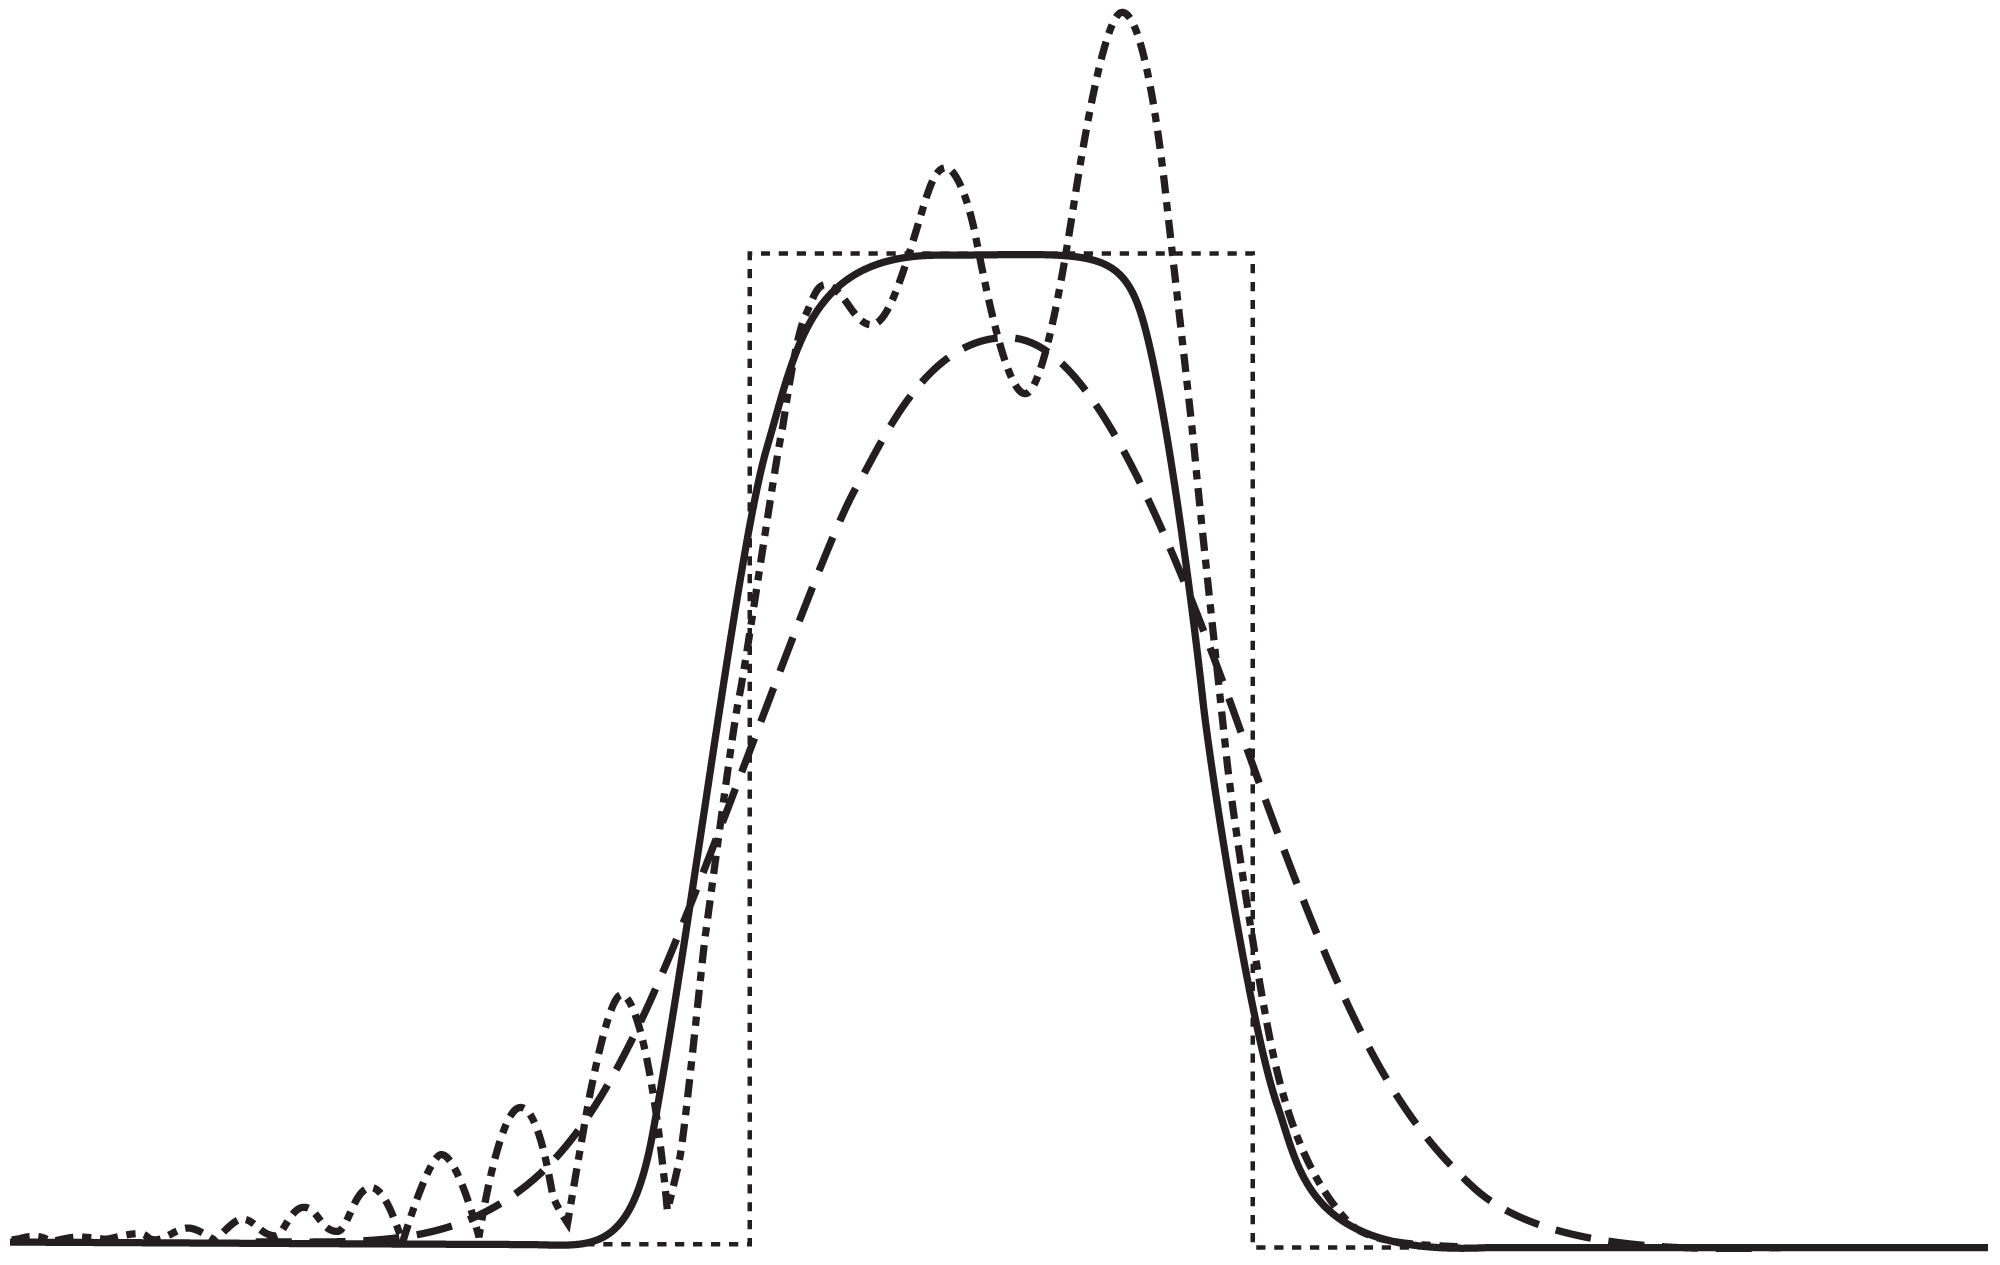
\includegraphics[width=0.75\textwidth]{png/hybrid-scheme-testing.png}}
\caption{Распространение прямоугольного импульса. Штриховая линия -- решение по схеме Куранта-Изаксона-Рис. Штрих-пунктирная -- решение по схеме Лакса-Вендрофа. Сплошная линия -- решение с использованием гибридной схемы. Точками показано точное решение.}
\label{pic:hybrid-scheme-testing}
\end{figure}

\subsubsection{Метод на неструктурированных сетках}

Идея сеточно-характеристического метода на неструктурированных сетках также основана на переносе инвариантов Римана вдоль направления характеристик. В ходе расчёта для каждой характеристики, выпущенной из точки на новом временном слое, по углу наклона $\lambda$ и шагу по времени $\tau$ определяется ячейка сетки на старом временном слое, в который попала данная характеристика (рис. \ref{pic:gcm_2d}). Простейшей формой ячейки неструктурированной сетки для двумерной постановки является треугольник, а для трёхмерной -- тетраэдр. В дальнейшем изложении будем ориентироваться на сетки из тетраэдров.

\begin{figure}[h]
\centering
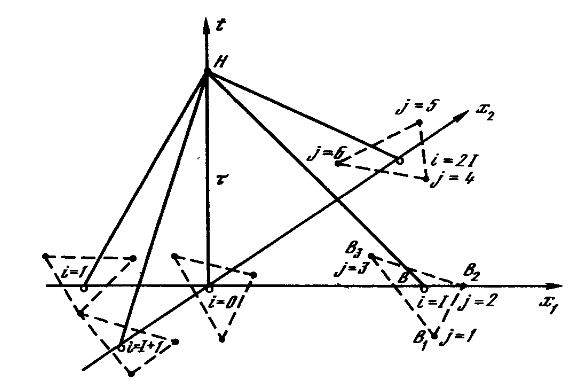
\includegraphics[width=0.6\textwidth]{png/characteristics-2d-triangles-inner.png}
\caption{Характеристики на неструктурированной сетке.}
\label{pic:gcm_2d}
\end{figure}

После того, как определён тетраэдр, в который попала характеристика, необходимо восстановить значение в точке пересечения характеристики со старым временным слоем. Для этого используется интерполяция значений в нужной точке по рассматриваемому тетраэдру. Подход к построению интерполяции высоких порядков на неструктурированных тетраэдральных сетках описан в работе Петрова И.Б. и Фаворская А.В. \cite{interpolation_3d}. Здесь описывается конструирование схемы интерполяции, непосредственно использовавшейся в данной работе.

Пусть искомая функция, задающая распределение в тетраэдре, является полиномом заданной степени $N$. Для линейной интерполяции (первый порядок точности по пространству) потребуется восстановить четыре коэффициента: постоянный член и множители перед $x, y, z$. Для квадратичной -- десять: те же четыре плюс еще шесть коэффициента перед $x^2, y^2, z^2, xy, xz, yz$. Для общего случая полинома степени $N$ количество коэффициентов в нем задается формулой $\frac{(N+1)(N+2)(N+3)}{6}$.

В произвольном тетраэдре $ABCD$ проведем плоскости, параллельные его сторонам, которые делят каждую из его сторон на $N$ частей (рис. \ref{pic:tetr-interpolation-base-points}). Количество точек внутри тетраэдра, в которых плоскости пересекаются между собой и со сторонами тетраэдраа, равно $\frac{(N+1)(N+2)(N+3)}{6}$. Именно эти точки пересечения мы выберем в качестве опорных, храня в них значения полинома, используемые для восстановления его величины во всех прочих точках.

\begin{figure}[h]
\centering
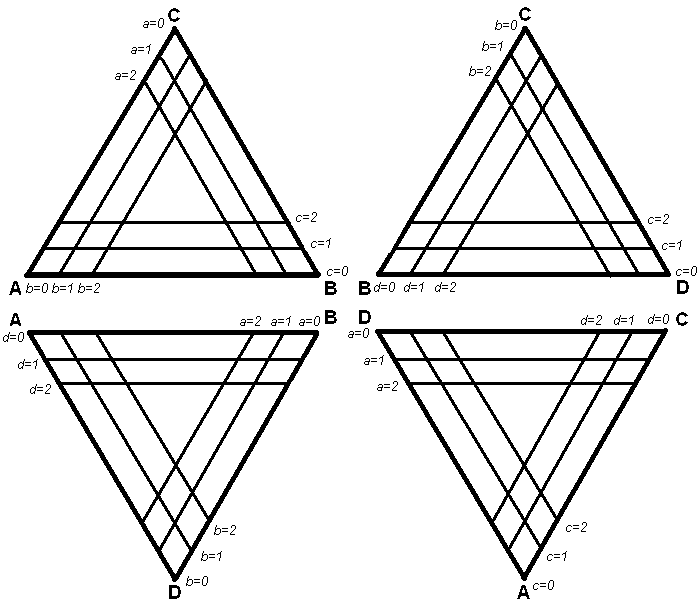
\includegraphics[width=0.5\textwidth]{png/tetr-interpolation-base-points.png}
\caption{Равномерное распределение опорных точек в тетраэдре (изображены стороны тетраэдра с проекциями плоскостей и их нумерацией).}
\label{pic:tetr-interpolation-base-points}
\end{figure}

Обозначим координаты вершин тетраэдра символами $\vec{r_A}, \vec{r_B}, \vec{r_C}, \vec{r_D}$, а ссылаться на опорные точки будем при помощи $r_{abcd}$. Индекс состоит из четырёх частей, каждая из которых описывает место пересечения плоскости, проходящей через опорную точку и параллельной определённой стороне, с соответствующим ребром тетраэдра (рис. \ref{pic:tetr-interpolation-base-points}). Для индексов любой опорной точки справедливо $a \ge 0, b \ge 0, c \ge 0, d \ge 0, a+b+c+d = N$.

Координаты опорной точки $r_{abcd}$ могут быть выражены через координаты вершин тетраэдра с использованием любой тройки индексов из четырех, достаточно взять систему координат с центром в одной из вершин и осями, проходящими через 3 другие.

Пусть необходимо реконструировать значение функции в произвольной точке $\vec{r}$ (обозначим её буквой $F$), которая может находиться как внутри тетраэдра, так и за его пределами. Введём в рассмотрение объёмы четырёх тетраэдров, которые формируются гранями исходного тетраэдра $ABCD$ и отрезками, соединяющими его вершины с точкой $F$.

Обозначим $V_i$ площадь того тетраэдра, одной из граней которого является грань исходного тетраэдра $ABCD$, противоположная его вершине $i$. Если $\vec{r}$ лежит внутри $ABCD$, то все четыре объёма $V_i$ положительны, в противном случае один или два «объёма» могут быть отрицательными. Но даже в этом случае, независимо от положения $\vec{r}$, их сумма будет равна объёму тетраэдра $ABCD$. Введём также относительные объёмы тех же тетраэдров $\nu_i = V_i / V$, где $V$ -- объём тетраэдра $ABCD$. Величины этих объёмов для точки $\vec{r}$, лежащей внутри $ABCD$, могут изменяться от нуля до единицы.

Значение функции в искомой точке $\phi(\vec{r})$ необходимо выразить через значения $\phi_{abcd} = \phi(r_{abcd})$, которые она принимает в опорных точках:
\begin{equation}
\phi(\vec{r}) = \sum_{a,b,c,d}{w_{abcd}(\vec{r}) \phi_{abcd}},
\end{equation}
где $w_{abcd}(\vec{r})$ -- вес опорной точки $\vec{r_{abcd}}$, также являющийся полиномом степени $N$. Вес обращается в единицу в одной опорной точке и в ноль во всех остальных опорных точках. Следующая функция веса удовлетворяет поставленным условиям:
\begin{equation}
w_{abcd}(\vec{r}) = \frac{ \prod_{i=1}^N{\nu_{T_i}(r) - \frac{n_i}{N}} }{ \prod_{i=1}^N{\nu_{T_i}(r_{abcd}) - \frac{n_i}{N}} }, \textrm{ где } T_i \in \{A, B, C, D\}, 0 \le n_i \le N
\end{equation}
при условии правильного подбора величин ${T_i}, {n_i}$. Принципиально, что если индексы двух опорных точек совпадают с точностью до перестановки, то функции их весов совпадают с точностью до той же перестановки величин в ${T_i}$.

\paragraph{Интерполяция первого порядка.} Опорные точки для линейной интерполяции -- $r_{1000}, r_{0100}, r_{0010}, r_{0001}$ (рис. \ref{pic:tetr-interpolation-1st-order-1}).

\begin{figure}[h]
\centering
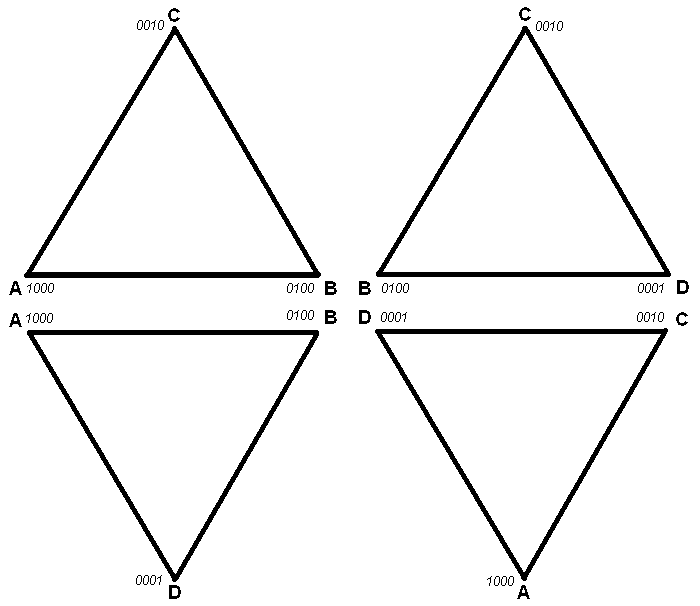
\includegraphics[width=0.5\textwidth]{png/tetr-interp-1st-order-1.png}
\caption{Опорные точки для интерполяции первого порядка.}
\label{pic:tetr-interpolation-1st-order-1}
\end{figure}

Найдём $w_{1000}(r)$ (рис. \ref{pic:tetr-interpolation-1st-order-2}):
\begin{equation}
w_{1000}(r) = \frac{ \nu_{T_1}(r) - n_1 }{ \nu_{T_1}(r_{1000}) - n_1 }.
\end{equation}

\begin{figure}[h]
\centering
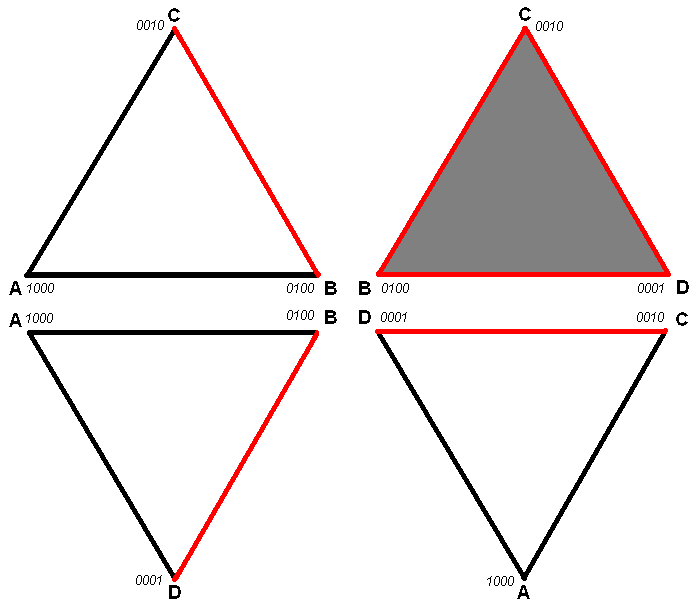
\includegraphics[width=0.5\textwidth]{png/tetr-interp-1st-order-2.png}
\caption{К вычислению весов для интерполяции первого порядка.}
\label{pic:tetr-interpolation-1st-order-2}
\end{figure}

Пусть $r = r_{0001}$. Подбираем $T_1$ и $n_1$:
\begin{align}
0 = \frac{ \nu_{T_1}(r_{0001}) - n_1 }{ \nu_{T_1}(r_{1000}) - n_1 } = \frac{ \nu_{A}(r_{0001}) - n_1 }{ \nu_{A}(r_{1000}) - n_1 } = \frac{0-n_1}{1-n_1} = \frac{0-0}{1-0} = \nu_{A}(r_{0001}).
\end{align}

Выполнив аналогичную процедуру для остальных весов, получаем:
\begin{align}
w_{1000}(r) = \nu_{A}(r) & & w_{0100}(r) = \nu_{B}(r), \nonumber\\
w_{0010}(r) = \nu_{C}(r) & & w_{0001}(r) = \nu_{D}(r).
\end{align}


\paragraph{Интерполяция второго порядка.} Опорные точки для квадратичной интерполяции -- $r_{2000}, r_{0200}, r_{0020}, r_{0002}, r_{1100}, r_{0110}, r_{0011}, r_{1001}, r_{1010}, r_{0101}$ (рис. \ref{pic:tetr-interpolation-2nd-order-1}).

\begin{figure}[h]
\centering
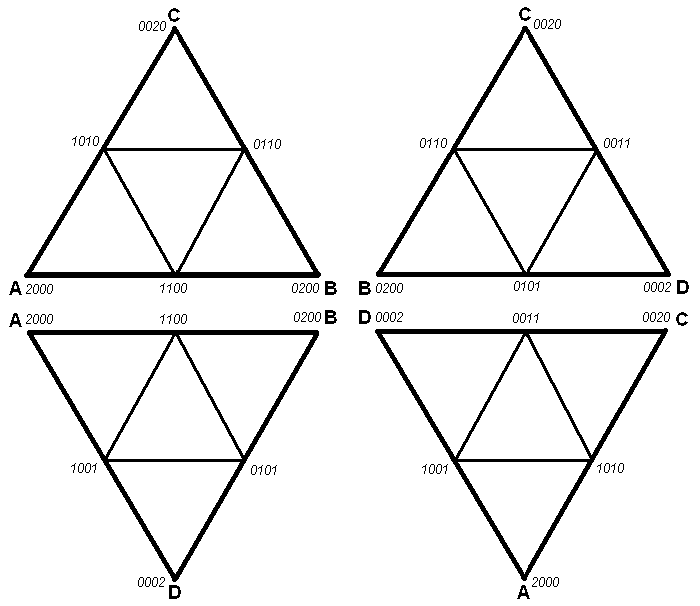
\includegraphics[width=0.5\textwidth]{png/tetr-interp-2nd-order-1.png}
\caption{Опорные точки для интерполяции второго порядка.}
\label{pic:tetr-interpolation-2nd-order-1}
\end{figure}


Найдём $w_{2000}(r)$:
\begin{equation}
w_{2000}(r) = \frac{ \nu_{T_1}(r) - \frac{n_1}{2} }{ \nu_{T_1}(r_{2000}) - \frac{n_1}{2} } \frac{ \nu_{T_2}(r) - \frac{n_2}{2} }{ \nu_{T_2}(r_{2000}) - \frac{n_2}{2} }.
\end{equation}


Пусть $r = r_{0002}$. Подбираем $T_1$ и $n_1$ (см. рис. \ref{pic:tetr-interpolation-2nd-order-2}а).

\begin{align}
0 = \frac{ \nu_{T_1}(r_{0002}) - \frac{n_1}{2} }{ \nu_{T_1}(r_{2000}) - \frac{n_1}{2} } = \frac{ \nu_{A}(r_{0002}) - \frac{n_1}{2} }{ \nu_{A}(r_{2000}) - \frac{n_1}{2} } = \frac{ 0 - \frac{n_1}{2} }{ 1 - \frac{n_1}{2} } = \frac{ 0 - \frac{0}{2} }{ 1 - \frac{0}{2} } = \nu_{A}(r_{0002}).
\end{align}

Таким образом, первый множитель $\nu_{A}(r)$.

Пусть $r = r_{1100}$. Подбираем $T_2$ и $n_2$ (см. рис. \ref{pic:tetr-interpolation-2nd-order-2}б).

\begin{align}
0 = \frac{ \nu_{T_2}(r_{1100}) - \frac{n_2}{2} }{ \nu_{T_2}(r_{2000}) - \frac{n_2}{2} } = \frac{ \nu_{A}(r_{1100}) - \frac{n_2}{2} }{ \nu_{A}(r_{2000}) - \frac{n_2}{2} } = \frac{ \frac{1}{2} - \frac{n_2}{2} }{ 1 - \frac{n_2}{2} } = \frac{ \frac{1}{2} - \frac{1}{2} }{ 1 - \frac{1}{2} } = 2\nu_{A}(r_{1100}) - 1.
\end{align}

Таким образом, второй множитель $2\nu_{A}(r)-1$.

Итого для веса $w_{2000}(r)$ получаем $w_{2000}(r) = \nu_{A}(r) (2\nu_{A}(r)-1)$. Остальные веса вершин тетраэдра получаются перестановкой индексов в данной формуле.

Найдём $w_{1100}(r)$:
\begin{equation}
w_{1100}(r) = \frac{ \nu_{T_1}(r) - \frac{n_1}{2} }{ \nu_{T_1}(r_{1100}) - \frac{n_1}{2} } \frac{ \nu_{T_2}(r) - \frac{n_2}{2} }{ \nu_{T_2}(r_{1100}) - \frac{n_2}{2} }.
\end{equation}

Пусть $r = r_{0002}$. Подбираем $T_1$ и $n_1$ (см. рис. \ref{pic:tetr-interpolation-2nd-order-2}в).

\begin{align}
0 = \frac{ \nu_{T_1}(r_{0002}) - \frac{n_1}{2} }{ \nu_{T_2}(r_{1100}) - \frac{n_1}{2} } = \frac{ \nu_{A}(r_{0002}) - \frac{n_1}{2} }{ \nu_{A}(r_{1100}) - \frac{n_1}{2} } = \frac{ 0 - \frac{n_1}{2} }{ \frac{1}{2} - \frac{n_1}{2} } = \frac{ 0 - \frac{0}{2} }{ \frac{1}{2} - \frac{0}{2} } = 2\nu_{A}(r_{0002}).
\end{align}

Таким образом, первый множитель $2\nu_{A}(r)$.

Пусть $r = r_{2000}$. Подбираем $T_2$ и $n_2$ (см. рис. \ref{pic:tetr-interpolation-2nd-order-2}г).

\begin{align}
0 = \frac{ \nu_{T_2}(r_{2000}) - \frac{n_2}{2} }{ \nu_{T_2}(r_{1100}) - \frac{n_2}{2} } = \frac{ \nu_{B}(r_{2000}) - \frac{n_2}{2} }{ \nu_{B}(r_{1100}) - \frac{n_2}{2} } = \frac{ 0 - \frac{n_2}{2} }{ \frac{1}{2} - \frac{n_2}{2} } = \frac{ 0 - \frac{0}{2} }{ \frac{1}{2} - \frac{0}{2} } = 2\nu_{B}(r_{2000}).
\end{align}

Таким образом, второй множитель $2\nu_{B}(r)$.

Итого для веса $w_{1100}(r)$ получаем $w_{1100}(r) = 4 \nu_{A}(r) \nu_{B}(r)$. Остальные веса дополнительных вершин получаются перестановкой индексов в данной формуле.



\begin{figure}[h]
\begin{subfigure}[b]{0.5\textwidth}
\centering
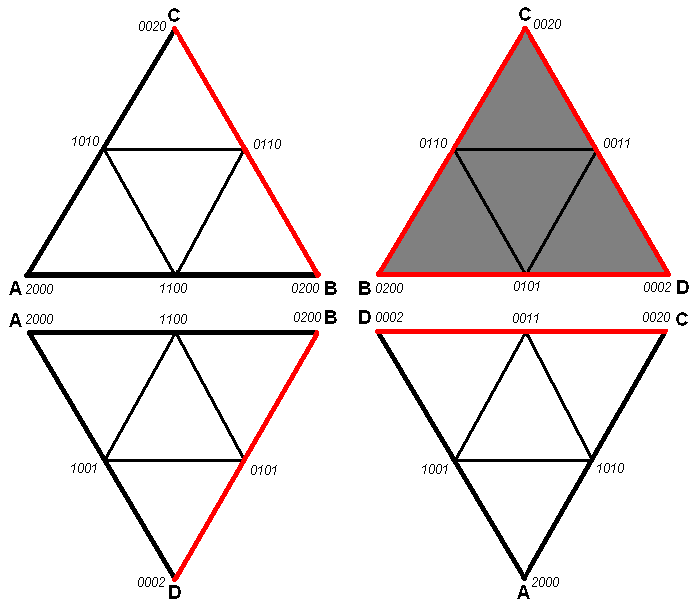
\includegraphics[width=\textwidth]{png/tetr-interp-2nd-order-2.png}
\caption{Схема для $w_{2000}(r)$ и $r = r_{0002}$}
\end{subfigure}
\begin{subfigure}[b]{0.5\textwidth}
\centering
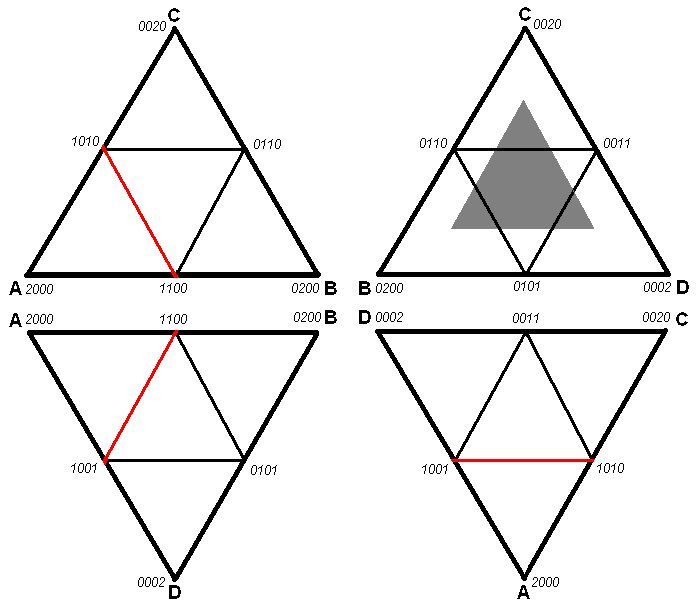
\includegraphics[width=\textwidth]{png/tetr-interp-2nd-order-3.png}
\caption{Схема для $w_{2000}(r)$ и $r = r_{1100}$}
\end{subfigure}
\begin{subfigure}[b]{0.5\textwidth}
\centering
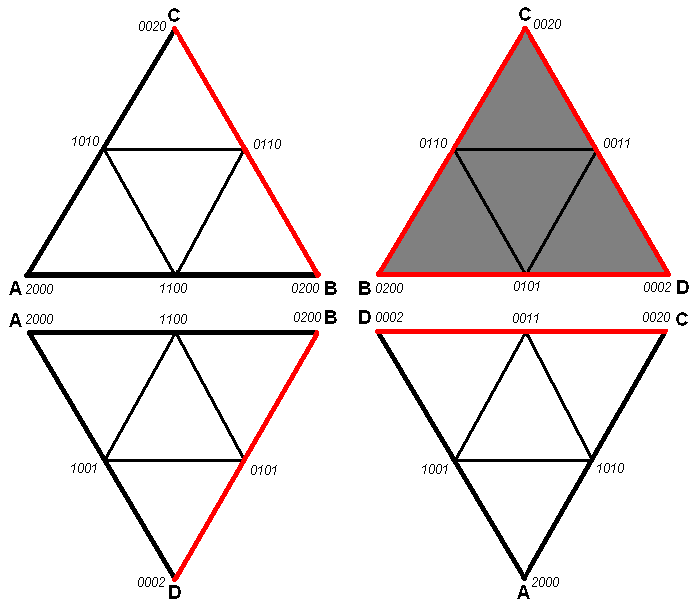
\includegraphics[width=\textwidth]{png/tetr-interp-2nd-order-4.png}
\caption{Схема для $w_{1100}(r)$ и $r = r_{0002}$}
\end{subfigure}
\begin{subfigure}[b]{0.5\textwidth}
\centering
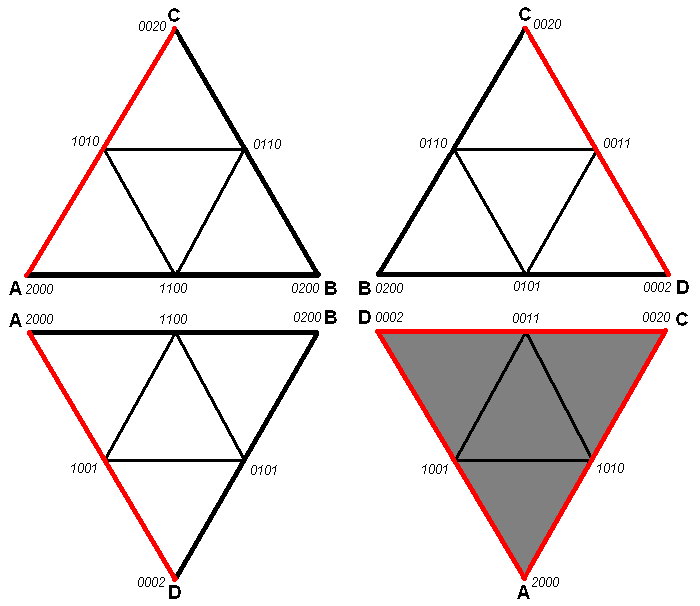
\includegraphics[width=\textwidth]{png/tetr-interp-2nd-order-5.png}
\caption{Схема для $w_{1100}(r)$ и $r = r_{2000}$}
\end{subfigure}
\caption{К вычислению весов для интерполяции второго порядка.}
\label{pic:tetr-interpolation-2nd-order-2}
\end{figure}

Итоговые веса для интерполяции второго порядка:
\begin{flalign}
w_{2000}(r) &=& \nu_{A}(r) (2\nu_{A}(r)-1) & & & w_{0200}(r) &=& \nu_{B}(r) (2\nu_{B}(r)-1), &\nonumber\\
w_{0020}(r) &=& \nu_{C}(r) (2\nu_{C}(r)-1) & & & w_{0002}(r) &=& \nu_{D}(r) (2\nu_{D}(r)-1), &\nonumber\\
w_{1100}(r) &=& 4 \nu_{A}(r) \nu_{B}(r) & & & w_{0110}(r) &=& 4 \nu_{B}(r) \nu_{C}(r), &\nonumber\\
w_{0011}(r) &=& 4 \nu_{C}(r) \nu_{D}(r) & & & w_{1001}(r) &=& 4 \nu_{D}(r) \nu_{A}(r), &\nonumber\\
w_{1010}(r) &=& 4 \nu_{A}(r) \nu_{C}(r) & & & w_{0101}(r) &=& 4 \nu_{B}(r) \nu_{D}(r). &
\end{flalign}


\paragraph{Интерполяция более высоких порядков.} Формулы для интерполяции более высоких порядков строятся аналогично. В данной работе используются схемы первого и второго порядка, поэтому вывод для более высоких порядков не приводится.

\paragraph{Гибридизация схемы.} Гибридная схема на неструктурированной сетке строится принципиально так же, как для структурированной. Используются две опорные схемы -- разобранные выше схемы с интерполяцией первого и второго порядка. В зависимости от локальной гладкости численного решения происходит переключение между схемами -- на гладких участках используется схема второго порядка, в области разрывов происходит переключение на схему первого порядка.


\subsubsection{Расчёт граничных узлов}

%\todo{Внятно написать эти два раздела}

Описанный метод подходит для расчёта внутренних узлов
сетки, т.е. только в том случае, если все характеристики, выпущенные из узла, не
выводит за пределы области интегрирования. В случае, когда узел находится на границе расчётной области, 
применяется иной подход для решения задачи. Рассматриваемая система
уравнений в граничных узлах области интегрирования имеет ровно три
\cite{chelnokov} выводящие характеристики. Поэтому для корректной постановки
задачи требуется задание граничных условий для каждого внешнего узла сетки в
количестве, равном числу выводящих характеристик. 

Граничные условия могут быть различными. В данной работе используется ряд граничных условий.

Свободная граница:
\begin{align}
\sigma_\tau=\sigma_n=0.
\end{align}
Здесь $\sigma_n$ и $\sigma_\tau$ -- нормальное и тангенциальное напряжение в граничной точке.

Заданная внешняя сила:
\begin{align}
\sigma_\tau &= \sigma_{\tau 0}, \nonumber\\
\sigma_n &= \sigma_{n 0}
\end{align}
Здесь $\sigma_{n 0}$ и $\sigma_{\tau 0}$ -- заданные извне нормальное и тангенциальное напряжение в граничной точке.

Заданная скорость границы:
\begin{align}
\vec{v} = \vec{v_0}.
\end{align}
Здесь $\vec{v_0}$ -- заданный извне вектор скорости в точке границы.


\subsubsection{Расчёт контактных узлов}

Расчёт контактной границы между двумя телами в целом аналогичен расчёту границы тела. Однако, в точке контакта присутствуют два узла -- по одному из каждого контактирующего тела. В каждом из них 6 уравнений исходной системы корректны, а 3 несовместны, так как соответствуют выводящим характеристикам. Кроме того, так как тела контактируют, для значений функции в двух рассматриваемых узлах есть уравнений связей. Уравнения связей должны задавать 6 условий, чтобы компенсировать 3 несовместные уравнения в каждом узле.

В результате получается система из 18 уравнений (6 у каждого узла и 6 уравнений связей) с 18 неизвестными (по 9 в каждом узле). Решая эту систему, получаем согласованные значения функции в обоих контактирующих узлах.

Уравнения связей могут быть различными, задавая различные условия контакта. В данной работе используется ряд контактных условий.

Скольжение тел друг относительно друга:
\begin{align}
v_n&=\tilde{v}_n,\nonumber\\
\sigma_n&=\tilde{\sigma}_n,\nonumber\\
\sigma_\tau&=\tilde{\sigma}_\tau=0.
\end{align}
Здесь $\sigma_n$ и $\sigma_\tau$ -- нормальное и тангенциальное напряжение в граничной точке. Символы с чертой относятся к первому телу, без черты -- ко второму.

Слипание тел:
\begin{align}
v_n&=\tilde{v}_n,\nonumber\\
v_\tau&=\tilde{v}_\tau.
\end{align}


\clearpage
\newpage

\subsection{Решение многомерной задачи}

\subsubsection{Схема с расщеплением по направлениям}

Система \ref{matrix_equation} (или что то же самое \ref{matrix_equation_generalized}) позволяет построить схему для решения трёхмерной задачи, если построены и исследованы одномерные схемы для задач:
\begin{equation}
\frac{\partial\vec{u}}{\partial{t}} + \mathbf{A}_{\xi_j} \frac{\partial\vec{u}}{\partial{\xi_j}} = 0.
\end{equation}

Такой подход называется расщеплением по направлениям и был предложен Р.П. Федоренко (\cite{fedorenko}). Идея метода решения исходной задачи состоит в замене исходной системы уравнений \ref{matrix_equation} одномерными системами -- тремя в случае отсутствия в исходной системе правой части и четырьмя, если правая часть имеется:
\begin{equation}
\frac{\partial}{\partial t}\vec u+\mathbf{A}_x \frac{\partial}{\partial x}\vec u = 0,
\label{matrix_equation_x}
\end{equation}
\begin{equation}
\frac{\partial}{\partial t}\vec u+\mathbf{A}_y \frac{\partial}{\partial y}\vec u = 0,
\label{matrix_equation_y}
\end{equation}
\begin{equation}
\frac{\partial}{\partial t}\vec u+\mathbf{A}_z \frac{\partial}{\partial z}\vec u = 0,
\label{matrix_equation_z}
\end{equation}
\begin{equation}
\frac{\partial}{\partial t}\vec u = \vec f.
\label{matrix_equation_f}
\end{equation}

Обозначим $F(\mathbf A_{\xi_1}, \mathbf A_{\xi_2}, \mathbf A_{\xi_3}, \vec f)$ оператор перехода между временными слоями $n$ и $n+1$, а $F_j(\mathbf A_{\xi_j}), j=1..3$ и $F_j(\vec f), j=4$ -- оператор, соответствующий $j$-ому уравнению в расщеплённой системе.

Необходимо сконструировать оператор $F$ из операторов $f_j, j=1..4$, обеспечив при этом аппроксимацию и устойчивость итоговой схемы, а также приемлемую вычислительную сложность алгоритма при его реализации.

Как разобрано выше, для каждой одномерной задачи существует ограничение на шаг по времени
\begin{equation}
\tau_j \le \frac{\min(h)}{\max(|\lambda_j|)},
\end{equation}

где $\min(h)$ -- минимальная высота тетраэдра в сетке, а $\max(|\lambda_j|)$ -- максимальное по модулю собственное число матрицы $\mathbf A_{\xi_j}$. Теоретически, в этом соотношении можно заменить $\min(h)$ на $\min(h_j)$ -- минимальное расстояние в направлении $j$-ой оси координат от узла сетки до точки пересечения с ближайшей гранью соседнего тетраэдра. Это расстояние может быть несколько больше, чем абсолютный минимум высоты по сетке $\min(h)$, и за счет этого обеспечивать несколько больший допустимый шаг по времени. Однако, на практике в силу случайной ориентации как тетраэдров сетки, так и координатных осей, потенциальное преимущество мало и не стоит того, чтобы усложнять алгоритм расчёта как логически из-за добавления новых элементов, так и вычислительно из-за необходимости постоянно определять новые точки пересечения.

При выполнении условия на $\tau_j$ схема, соответствующая оператору $F_j$, устойчива и имеет свой порядок аппроксимации по времени и пространству для одномерной задачи. Теперь рассмотрим различные варианты составления оператора $F$ из $F_j$.


\subsubsection{Схема с расщеплением первого порядка}

В простейшем случае можно сложить операторы $F_j$ с коэффициентами $a_j$. При таком подходе получаем:
\begin{align}
F(\mathbf A_{\xi_1}, \mathbf A_{\xi_2}, \mathbf A_{\xi_3}, \vec f) &= \sum\limits_{j} a_j F_j(\frac{1}{a_j} \mathbf A_{\xi_j}), \nonumber\\
\sum\limits_{j} a_j &= 1, \nonumber\\
a_j &> 0.
\end{align}

Такая схема обеспечивает первый порядок аппроксимации итогового оператора $F$, если в качестве $F_j$ были выбраны схемы как минимум первого порядка. В выборе $a_j$ присутствует определённый произвол, что позволяет использовать их для получения максимального шага по времени.

Действительно, собственные числа матриц $\mathbf A_{\xi_j}^* = \frac{1}{a_j} \mathbf A_{\xi_j}$ будут в $a_j$ раз отличаться от собственных чисел исходных матриц $\mathbf A_{\xi_j}$. Максимально допустимый шаг по времени
\begin{equation}
\tau \le \max{\tau_j} = \frac{\min(h)}{\max(|\lambda_j^*|)} = \frac{\min(h)a_j}{\max(|\lambda_j|)}.
\end{equation}

Таким образом, для максимизации допустимого шага получаем условие:
\begin{equation}
\frac{a_1}{\max(|\lambda_1|)} = \frac{a_2}{\max(|\lambda_2|)} = \frac{a_3}{\max(|\lambda_3|)}.
\end{equation}

Откуда следует
\begin{align}
a_j = \frac{\max(|\lambda_j|)}{\max(|\lambda_1|)+\max(|\lambda_2|)+\max(|\lambda_3|)},\nonumber\\
\tau = \frac{\min(h)}{\max(|\lambda_1|)+\max(|\lambda_2|)+\max(|\lambda_3|)}
\end{align}

Видно, что при таком конструировании расщепления получается вычислительно простой алгоритм -- требуется только вычислить независимое воздействие операторов $F_j$ на временном слое $n$, чтобы потом получить значение на временном слое $n+1$ как их сумму. Однако, схема обеспечивает только первый порядок аппроксимации $F$, даже если отдельно $F_j$ имеют более высокий порядок. Кроме того, допустимый шаг по времени заметно уменьшается (как правило, в 3 раза, так как $\max(|\lambda_j|)$ одинаково для всех матриц $\mathbf A_{\xi_j}$.


\subsubsection{Схема с расщеплением второго порядка}

Для обеспечения второго порядка аппроксимации итоговой схемы необходимо операторы $F_j$ не сложить, а перемножить
\begin{align}
\label{split_scheme_2nd_order}
F(\mathbf A_{\xi_1}, \mathbf A_{\xi_2}, \mathbf A_{\xi_3}, \vec f) = F_1(\mathbf A_{\xi_1}) F_2(\mathbf A_{\xi_2}) F_3(\mathbf A_{\xi_3}).
\end{align}

С точки зрения реализации это означает, что сначала к значениям на временном слое $n$ применяется первый оператор, потом к результату действия первого оператора -- второй, к результату второго -- третий. Значения, полученные после применения всех операторов, являются значениями на новом временном слое $n+1$:
\begin{align}
\vec u^{'} &= F_1(\mathbf A_{\xi_1}) \vec u^n, \nonumber\\
\vec u^{''} &= F_2(\mathbf A_{\xi_2}) \vec u^{'}, \nonumber\\
\vec u^{n+1} &= F_3(\mathbf A_{\xi_3}) \vec u^{''}.
\end{align}

Допустимый шаг по времени определяется минимальным допустимым шагом по времени для схем $F_j$:
\begin{align}
\tau = \min\limits_{j}(\tau_j) = \min\limits_{j}(\frac{\min(h)}{\max(|\lambda_j|)}) = \frac{\min(h)}{\max\limits_{j}\max(|\lambda_j|)}.
\end{align}

Таким образом, расщепление данного вида обеспечивает второй порядок аппроксимации и не приводит к уменьшению допустимого шага по времени. Однако, если использовать схему в виде \ref{split_scheme_2nd_order}, то очевидным образом возникает несимметрия решения, так как направления координатных осей перестают быть равноправными.

Метод симметризации схемы достаточно очевиден -- необходимо использовать не одно произведение операторов, которое порождает выделенные направления, а усреднять все возможные перестановки операторов $F_j$:
\begin{align}
\label{split_scheme_2nd_order_sym}
F(\mathbf A_{\xi_1}, \mathbf A_{\xi_2}, \mathbf A_{\xi_3}, \vec f) = \frac{1}{6} \sum\limits_{i \ne j \ne k} F_i(\mathbf A_{\xi_i}) F_j(\mathbf A_{\xi_j}) F_k(\mathbf A_{\xi_k}).
\end{align}

Такая схема становится симметричной, но теперь приходится считать действие операторов $F_j$ 18 раз вместо 3 раз.


\subsubsection{Схема с расщеплением и случайным выбором базиса}

Альтернативным способом симметризации схемы \ref{split_scheme_2nd_order} является случайный выбор базиса. В этом случае схема расщепления обеспечивает второй порядок аппроксимации многомерной задачи и возможность использовать большое значение $\tau$. Случайный выбор базиса обеспечивает отсутствие выделенных направлений и симметричность решения. За счет этого на каждом временном шаге требуется вычислять только 3 оператора $F_j$.

Обратной стороной такого подхода, который проявляется при практической реализации метода, является тот факт, что в случайно выбранном базисе из-за изменения направлений осей постоянно меняются точки на предыдущем временном слое, в которые попадают характеристики и по которым производится реконструкция решения. В результате требуется искать эти точки заново после смены базиса на каждом шаге. Однако, при разумной организации структур данных, вычислительная сложность этой операции достаточно невелика и такой подход оказывается значительно экономичнее, чем вычисление операторов $F_j$ дополнительные 15 раз.

\clearpage
\newpage

\subsection{Движение сетки}

%\todo{Переписать слова ниже. Объяснить внятно про конвективные члены.}

В случае конечных деформаций существует несколько подходов к описанию движения точек среды.

Эйлерова сетка строится однократно и в дальнейшем не изменяется. Это может быть наилучшим решением для тел с фиксированными границами. Для решения задач с конечными деформациями границ выбирают наиболее простую форму эйлеровой сетки — декартову решетку, потому что, независимо от формы ячеек, неподвижные узлы и ребра сетки не будут совпадать в каждый момент времени с движущимися границами, и неизбежны сложности, описанные для декартовых решеток.

Точки лагранжевой сетки смещаются вместе с точками тела, поэтому границы тела всегда совпадают с сеточными линиями. Однако при наличии сдвиговых деформаций в теле, ячейки лагранжевой сетки могут постепенно вырождаться и пересекать друг друга. Численные методы при вырождении сетки обнаруживают неустойчивость и счет приходится прекращать. Поэтому неизбежен подход, называемый лагранжева сетка с перестройкой, в котором, как только детектируется приближение сетки к вырожденному состоянию, производится построение новой сетки, а значения в новых узлах интерполируются из прежних значений. Процедура интерполяции сама по себе приводит к потере точности решения, поэтому желательно перестраивать сетку как можно реже. Ниже будет предложен альтернативный способ решения проблемы больших деформаций, который вместо перестроения сетки использует динамический выбор сеточного шаблона в зависимости от локальных свойств решения.

Подвижная сетка является обобщением лагранжевой, ее точки движутся от слоя к слою с ненулевыми скоростями и смещаются как относительно неподвижной системы координат, так и относительно точек тела. Их движение может быть подобрано таким образом, чтобы исключить вырождение сетки со временем. Однако использование подвижной сетки требует вносить изменения в решаемые уравнения для учета конвективных членов.

Расчет на лагранжевой сетке из тетраэдров подразумевает, что скорость смещения вершин сетки совпадает со скоростью среды. Но в методах второго порядка и выше вводятся дополнительные узлы, отличные от вершин, движение которых задается линейной интерполяцией движений вершин тетраэдра, в котором они расположены. Даже если скорость всех вершин является лагранжевой, то узлы, не совпадающие с вершинами, смещаются относительно точек среды. Это означает, что при их расчете необходимо учитывать конвективные члены. Отличие скорости этих узлов от скорости среды невелико: $O(h^2)$, где $h$ — мелкость сетки. Собственные значения матриц при поправке на конвекцию также изменятся на $O(h^2)$.

Отличие мест пересечения характеристики до и после поправки со слоем $t^n$ составит $\tau O(h^h2) = O(\tau^3)$, такого же порядка и отличие в восстанавливаемом интерполяцией решении. Поэтому в методе второго порядка можно не рассматривать отличие движения узлов в центре ребер от лагранжевых — это не понизит степень аппроксимации, а в методах третьего порядков и выше поправка необходима.

\clearpage
\newpage

\subsection{Выделение контактных границ}

При взаимном движении тел, а также в задачах с конечными деформациями отдельной задачей становится построение алгоритма явного выделения контактных границ. Стандартный подход (именно он использован в этой работе) к реализации состоит из двух этапов:
\begin{itemize}
	\item грубое (см. рис. \ref{pic:collision_detection}) определение областей потенциально возможного контакта при помощи AABB\footnote{AABB (Axis-aligned bounding box) -- ограничивающий параллелепипед, выровненный по осям };
	\item уточнение контактирующих узлов внутри найденных областей.
\end{itemize}
\begin{figure}[htp]
\centering
\includegraphics[width=0.6\textwidth]{eps/collision_detection.eps}
\caption{Использование AABB для грубого определения областей контакта. На
рисунке изображены тела $B_1$ и $B_2$, а также AABB, построенные для контуров
$C_1$ и $C_2$ этих тел. Контакты ищутся в пересечении разных AABB.}
\label{pic:collision_detection}
\end{figure}
По пересечению AABB определяются пары <<потенциально>> находящихся в контакте тел. Затем для каждой найденной пары проводится уточнение зоны контакта: проверяются <<на контакт>> все пары узлов одного тела и треугольников поверхности другого. Пары <<контактирующих>> узлов и треугольников определяются полным перебором по <<кандидатов>>, попавших внутрь пересечения AABB. Под контактом точки и треугольника здесь понимается следующее: считаем, что треугольник и точка контактируют, если зона влияния (сфера заранее выбранного радиуса) точки пересекает треугольник (см. рис. \ref{pic:contact_detection}).
\begin{figure}[htp]
\centering
\includegraphics[width=0.6\textwidth]{pdf/contact_detection.pdf}
\caption{Определение контакта.}
\label{pic:contact_detection}
\end{figure}
Если треугольник и точка находятся в контакте, то следующим шагом строится парный виртуальный узел -- этот узел лежит внутри контактирующего треугольника так, чтобы прямая проходящая через реальный и виртуальный узлы, являлась нормалью к треугольнику (см. рис. \ref{pic:contact_processing}).
\begin{figure}[htp]
\centering
\includegraphics[width=0.6\textwidth]{pdf/contact_processing.pdf}
\caption{Построение виртуальных узлов при обработке контактирующих границ.}
\label{pic:contact_processing}
\end{figure}
После того, как виртуальный узел построен, получаются значения всех величин в нём. Для этого в данной работе использовалась линейная интерполяция при помощи барицентрических координат. Задача заключается в следующем (см. рис. \ref{pic:triangle_interpolation}): есть треугольник и точка, лежащая в его плоскости, в трёхмерном пространстве, нужно, используя известные значения в вершинах треугольника, определить значение в точке.
\begin{figure}[htp]
\centering
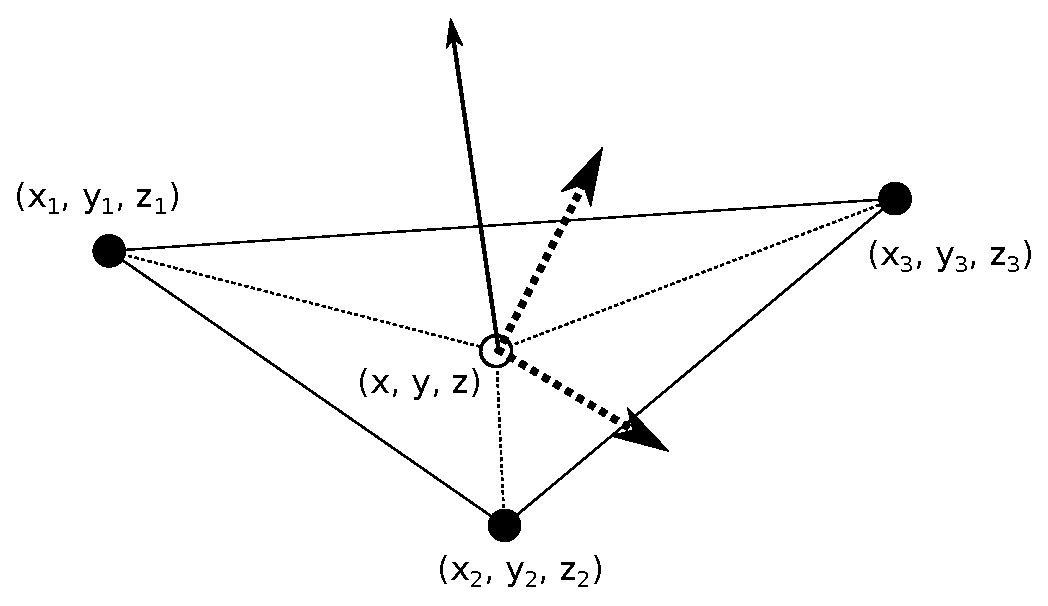
\includegraphics[width=0.6\textwidth]{eps/triangle_interpolation.eps}
\caption{Выбор новых осей координат при интерполяции в треугольнике.}
\label{pic:triangle_interpolation}
\end{figure}
В работе используется следующий подход для реализации интерполяции:
\begin{itemize}
	\item поворотом осей координат добиваемся того, чтобы все четыре точки имели одинаковую координату $\tilde{x}$;
	\item используем интерполяцию в плоскости через барицентрические координаты.
\end{itemize}
Пусть $\vec{n}=(n_1,n_2,n_3)$ -- нормаль к плоскости треугольника, тогда в системе координат с базисными векторами:
\begin{align}
\label{eq:new_coords}
\vec{\tilde{e}}_1&=(n_1, n_2, n_3), \nonumber \\
\vec{\tilde{e}}_2&=(n_3, 0, -n_1), \nonumber \\
\vec{\tilde{e}}_3&=(n_1*n_2, -n_1^2-n_3^2, n_2*n_3)
\end{align}
все четыре точки имеют одинаковую координату $\tilde{x}$. Такую систему
координат невозможно использовать, если $n_1=n_3=0$, но в этом случае все точки
имеют одинаковую координату $y$, поэтому, сделав замену
\begin{align}
\label{eq:new_coords_2}
\tilde{x}&=y \nonumber\\
\tilde{y}&=x \nonumber \\
\tilde{z}&=z,
\end{align}
придём опять к ситуации, когда все четыре точки имеют одинаковую координату $x$.
После этих преобразований значение в точке $(x,y,z)$ может быть вычислено по формуле
\begin{equation}
\label{eq:triangle_interpolation}
v=v_1*\lambda_1+v_2*\lambda_2+v_3*\lambda_3, 
\end{equation}
где $v_1,v_2,v_3$ -- значения в вершинах треугольника, а $\lambda_1,\lambda_2,\lambda_3$ -- барицентрические координаты
\begin{align}
\label{eq:barycentric_coords}
\lambda_1&=\frac{(y_2-y_3)(x-x_3)+(x_3-x_2)(y-y_3)}{(y_2-y_3)(x_1-x_3)+(x_3-x_2)(y_1-y_3)}, \nonumber \\
\lambda_2&=\frac{(y_3-y_1)(x-x_3)+(x_1-x_3)(y-y_3)}{(y_2-y_3)(x_1-x_3)+(x_3-x_2)(y_1-y_3)}, \nonumber \\
\lambda_3&=1-\lambda_1-\lambda_2.
\end{align}
Эта интерполяция обладает первым порядком точности, что согласуется с порядком точности остальных частей алгоритма.


\clearpage
\newpage


\subsection{Расчёт с шагом $\tau > h/\lambda$}

\subsubsection{Необходимость расчёта с шагом $\tau > h/\lambda$}

Одной из принципиальных проблем, с которыми сталкивается метод характеристик на сетках из тетраэдров при попытке расчета им реальных задач, является низкое качество сеток, создаваемых стандартными генераторами сеток. Данный вопрос практически всегда остается за рамками в любых публикациях по теме сеточно-характеристических методов, так как не связан непосредственно с конструированием самого метода. Тем не менее, для практики эта проблема крайне важна, поэтому остановимся на ней подробнее.

Если подходить к вопросу формально, то сеточно-характеристический метод может использоваться на любой сетке из тетраэдров. Однако, как было рассмотрено выше, для сеток из тетраэдров имеет место ограничение на шаг по времени, аналогичное курантовскому шагу для равномерной прямоугольной сетки. Так для каждого узла сетки:

\begin{equation}
\tau \le \frac{\min(h)}{\max(|\lambda|)},
\end{equation}

где $\min(h)$ -- минимальная высота тетраэдра, в которые входит данный узел, $\max(|\lambda|)$ -- максимальное по модулю собственное число матрицы $\mathbf A$ для данного узла.

С практической точки зрения крайне нежелательна ситуация, когда $\tau$ оказывается малым для отдельных узлов сетки, так как это накладывает ограничения на шаг по времени для всей сетки. Разумеется, необходимо различать случай, когда малый шаг по времени продиктован объективными требованиями высокого разрешения по времени и пространству, и случай, когда он является нежелательным следствием тех или иных проблем. В данный момент мы сосредоточимся на втором случае.

В таблице \ref{tbl:mesh-stats-summary} приведены данные по сеткам из тетраэдров, созданных в кубе с ребром 10 с помощью различных генераторов. Во всех случаях было задано значение мелкости сетки $h_* = 0.25$. В идеальном случае была бы построена сетка из правильных тетраэдров одинакового размера с высотами ровно равными $h_*$. Если такое оказалось бы возможно, то шаг по времени точно соответствовал бы ожидаемому $\tau_* \le h_* / \lambda$ и зависел бы только от реологии среды (значения $\lambda$). Очевидно, что в случае реальной геометрии построить сетку полностью из правильных тетраэдров одного размера невозможно, поэтому следует ожидать появления тетраэров размером несколько больше или меньше, чем заданный, а также тетраэдров с искажениями относительно правильной формы. Полученная в итоге минимальная высота тетраэдра определяет шаг по времени для всей сетки $\tau \le \min(h) / \lambda$. В связи с этим логично ввести критерий качества сетки в следующем виде:

\begin{equation}
q = \frac{\min(h)}{h_*},
\end{equation}

где $h_*$ -- заданная желаемая мелкость сетки, а $\min(h)$ -- минимальная высота в сетке, фактически выданной генератором.

Для идеальной сетки $q = 1$. В случае не слишком больших отклонений от единицы сетку можно считать <<достаточно хорошей>> для расчёта. Однако, как видно из таблицы \ref{tbl:mesh-stats-summary}, на практике даже для простейшей геометрии $q$ находится в диапазоне $0.00065 \le q \le 0.126$. Это приводит к неоправданному падению шага по времени на 1-3 порядка и, соответственно, к необоснованному росту требуемого объема вычислений. Приведенные гистограммы распределения высот тетраэдров в полученных сетках (рис. \ref{pic:mesh_quality}) показывают, что проблема не связана с наличием единичных вырожденных тетраэдров, а носит систематический характер.

Причиной такого низкого качества сеток является тот факт, что все существующие генераторы сеток ориентированы на построение сеток для метода конечных элементов. Для МКЭ критерии качества сетки совершенно иные -- для эффективной работы метода требуется, чтобы их углы были максимально близки к правильным, а линейные размеры при этом могут быть любыми. Соответственно, ориентированные на МКЭ алгоритмы построения сеток оказываются неэффективными с точки зрения сеточно-характеристического метода.

Очевидным способом решения данной проблемы может быть разработка алгоритмов построения сеток, ориентированных на улучшения качества в терминах сеточно-характеристического метода. Однако в данной работе предлагается другой подход -- модификация метода для обеспечения эффективной работы на сетке низкого качества. Данный подход, как будет рассмотрено ниже, может применяться не только для решения проблемы малого шага по времени из-за низкого качества изначальной сетки, но и в случае деградации шага по времени из-за вырождения сетки в зоне больших деформаций.

\begin{table}[h]
\centering
\caption{Качество сеток, созданных различными генераторами в кубе с ребром 10}
\begin{tabular}{|c|c|c|c|}
\hline
Генератор & Заданное $H$ & $\min(H)$ & $\max(H)$ \\
\hline
gmsh & 0.25 & 0.000845531 & 0.307492 \\
tetgen & 0.25 & 0.0315793 & 0.279029 \\
Ani3D & 0.25 & $1.08e^{-8}$ & 3.63429 \\
Ani3D + косметика & 0.25 & 0.000162557 & 3.7205 \\
\hline
\end{tabular}
\label{tbl:mesh-stats-summary}
\end{table}


\begin{figure}[htp]
\begin{subfigure}[b]{0.5\textwidth}
\centering
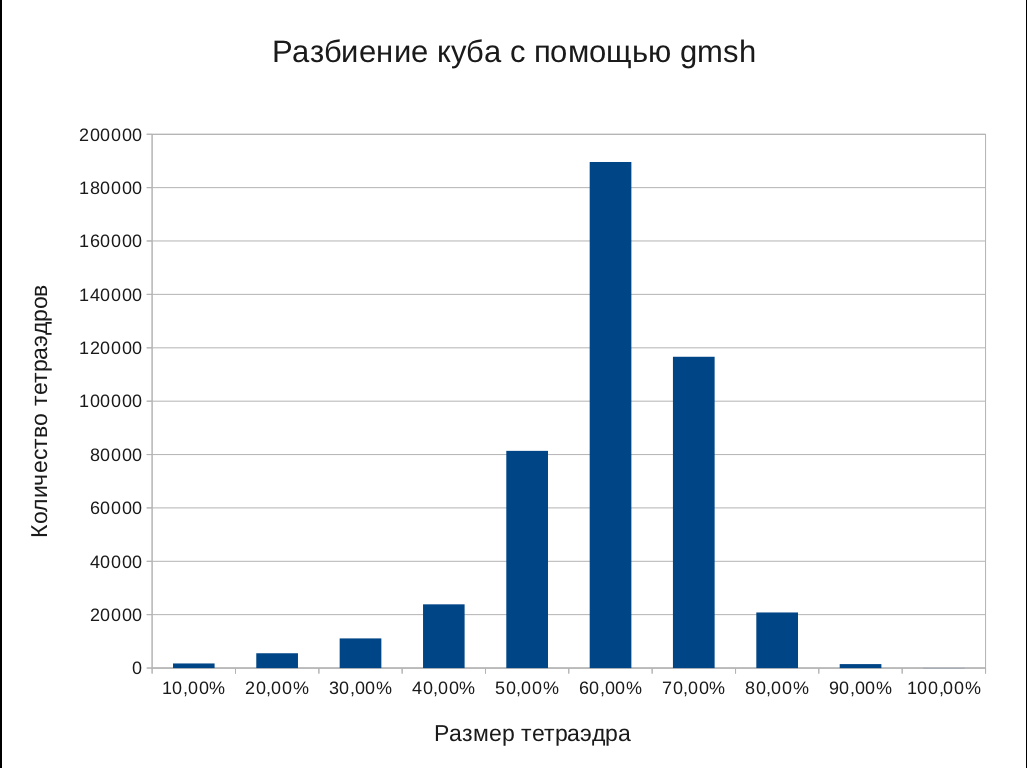
\includegraphics[width=\textwidth]{png/gmsh-stats.png}
\caption{Генератор gmsh.}
\end{subfigure}
\begin{subfigure}[b]{0.5\textwidth}
\centering
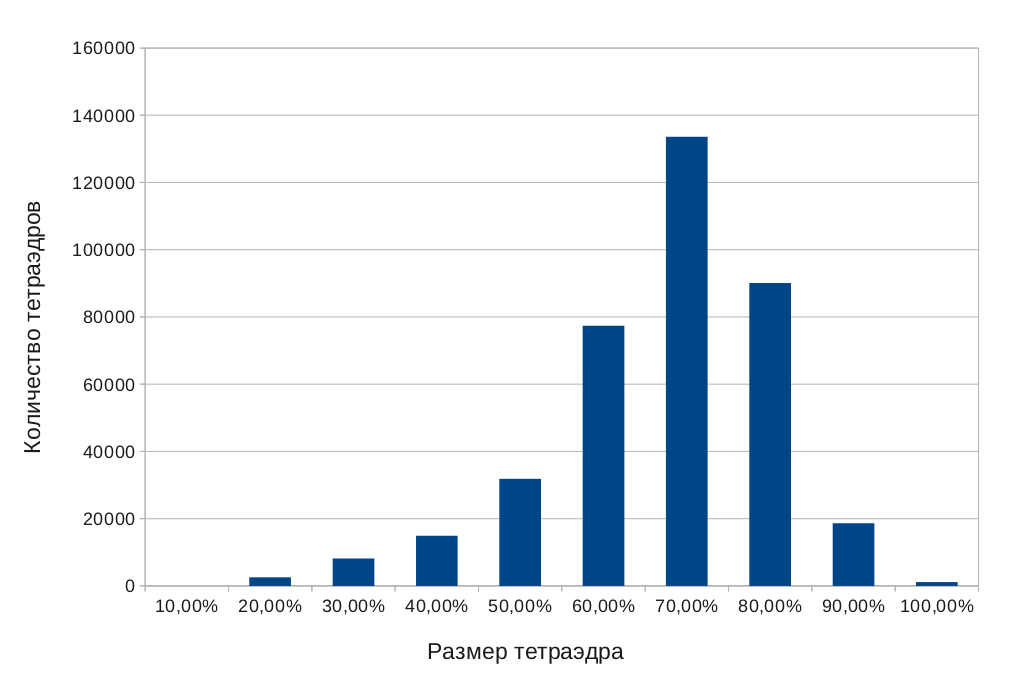
\includegraphics[width=\textwidth]{png/tetgen-stats.png}
\caption{Генератор tetgen.}
\end{subfigure}
\begin{subfigure}[b]{0.5\textwidth}
\centering
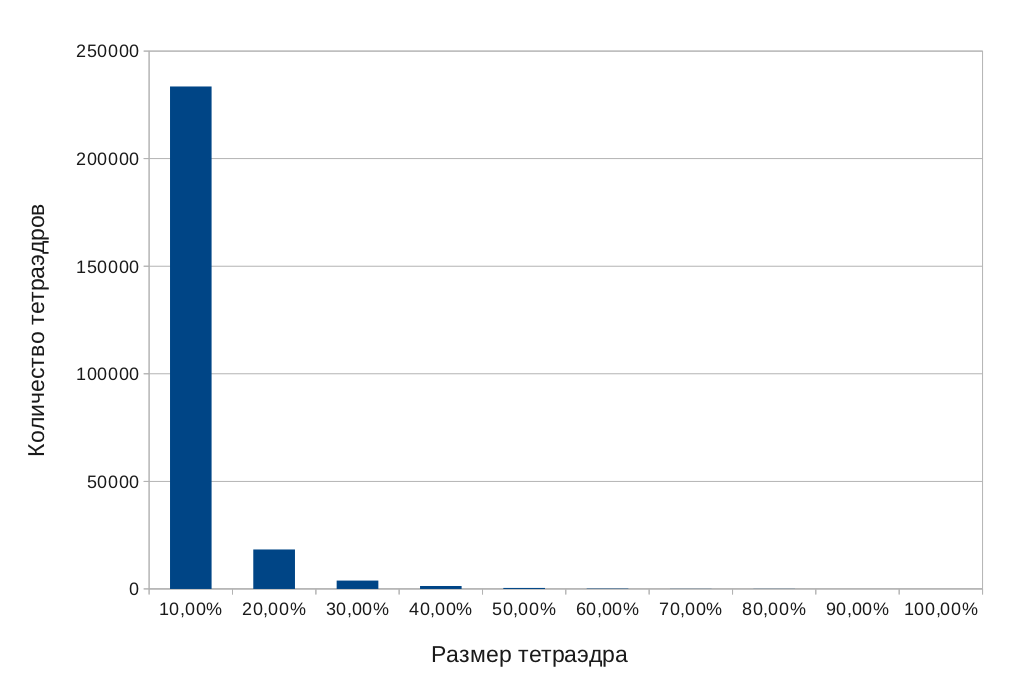
\includegraphics[width=\textwidth]{png/ani3d-stats.png}
\caption{Генератор Ani3D.}
\end{subfigure}
\begin{subfigure}[b]{0.5\textwidth}
\centering
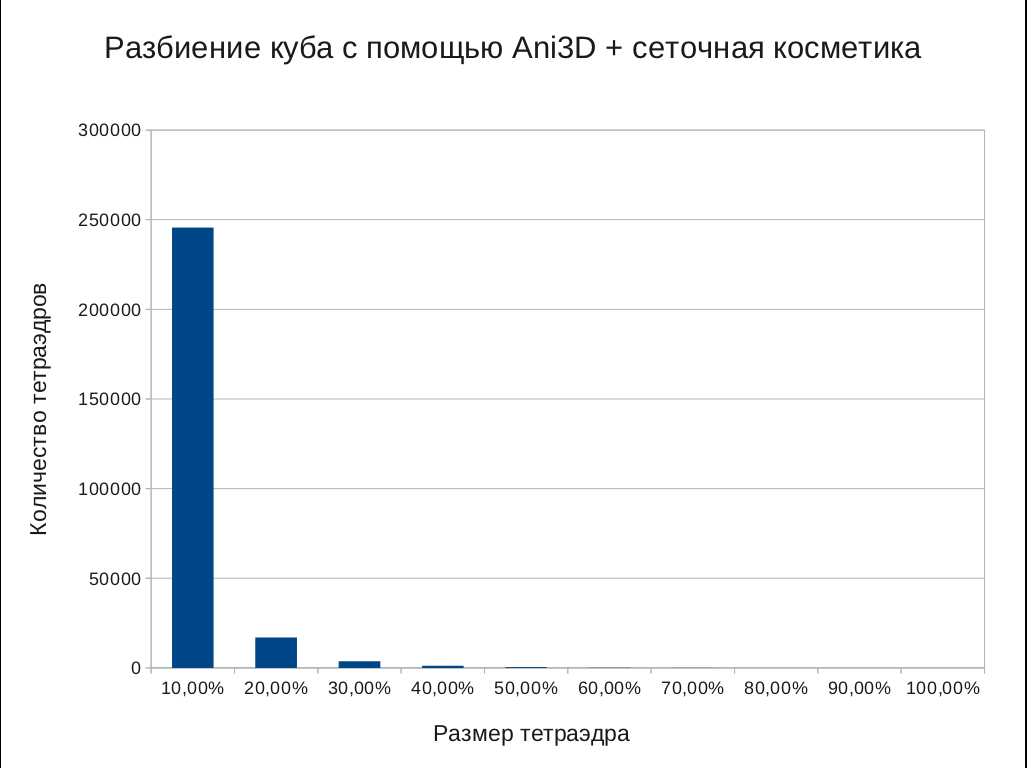
\includegraphics[width=\textwidth]{png/ani3d-improved-stats.png}
\caption{Генератор Ani3D с сеточной косметикой.}
\end{subfigure}
\caption{Сетка в кубе, созданная различными генераторами. Распределение тетраэдров по размеру.}
\label{pic:mesh_quality}
\end{figure}

\clearpage
\newpage

\subsubsection{Конструирование метода}

Рассмотрим одномерное уравнение переноса

\begin{equation}
\frac{\partial{u}}{\partial{t}} + \lambda \frac{\partial{u}}{\partial{x}} = 0, \lambda \ne const.
\end{equation}

Введем в области интегрирования разностную сетку и обозначим $u_m^n = u(t^n, x_m)$. Обратим внимание, что мы изначально предполагаем неравномерность сетки. Это соответствует как случаю с изначально сеткой низкого качества, так и случаю больших деформаций и вырождения сетки. Кроме того, мы рассматриваем случай разных значений $\lambda$ в разных точках расчетной области. Такая ситуация имеет место, если среда изначально неоднородная или если большие деформации вызвали значительное локальное изменение плотности в точке.

Особенностью предлагаемого метода является тот факт, что на данном этапе не будем выбирать фиксированный сеточный шаблон. Необходимые точки на предыдущем временном слое, по которым выполняется реконструкция значений на следующем шаге по времени, будут определяться в ходе вычислений отдельно для каждой рассчитываемой точки, исходя из локальных свойств решения в ней.

Пусть из тех или иных соображений был выбран шаг по времени $\tau$, такой что характеристика из точки $u_m^n$ на новом временном слое не попадает в отрезок $(u_{m-1}^n; u_{m+1}^n)$. Такая ситуация имеет место в <<маленьких>> тетраэдрах сетки низкого качества, если шаг по времени был выбран ориентируясь на <<средние>> тетраэдры сетки.

В этом случае найдем тот отрезок $(u_{m-k-1}^n; u_{m-k}^n)$, в котором выпущенная характеристика пересекает временной слой $n$. Точку пересечения обозначим $x^*$. Также введем обозначения:
\begin{align}
x_{m-k} - x_{m-k-1} &= h_k,\nonumber\\
x_m - x^* = \lambda \tau &= l_0,\nonumber\\
x_m - x_{m-k} &= l_k.
\end{align}

Нормируя $l_k$ и $l_0$ на $h_k$ получаем:
\begin{align}
q_0 &= l_0 / h_k = \lambda \tau / h_k = \sigma,\nonumber\\
q_k &= l_k / h_k,
\end{align}
где $\sigma$ -- аналог классического числа Куранта для равномерной сетки.

Рассмотрим простейший случай линейной интерполяции значения в точке $u_*^n$ по точкам  $u_{m-k-1}^n$ и $u_{m-k}^n$. Получаем для значения на новом временном слое $u_m^{n+1}$ следующее выражение:
\begin{align}
\label{newmethod_1d_scheme}
u_m^{n+1} = u_*^n = (q_k + 1 - q_0) u_{m-k}^n + (q_0 - q_k) u_{m-k-1}^n.
\end{align}


\subsubsection{Исследование метода}

Чтобы найти порядок аппроксимации по времени и по пространству используем разложение $u_{m+\mu}^{n+\nu}$ в ряд Тейлора. Обозначим:
\begin{align}
q_0 - q_k &= \sigma_k,\nonumber\\
\frac{h_k}{l_0} &= \alpha,\nonumber\\
\frac{l_k}{l_0} &= \beta,
\end{align}
где очевидно $\alpha < 1, \beta < 1$.

Раскладывая \ref{newmethod_1d_scheme} в ряд Тейлора в окрестности $u = u_m^n$ до второго порядка малости получаем:
\begin{align}
u + u_\tau \tau + u_{\tau\tau} \frac{\tau^2}{2} &= (1 - \sigma_k) (u - l_k u_x + u_{xx} \frac{l_k^2}{2}) + \nonumber\\
	&+ \sigma_k (u - (l_k+h_k) u_x + u_{xx} \frac{(l_k+h_k)^2}{2}) \nonumber\\
u_\tau \tau + u_{\tau\tau} \frac{\tau^2}{2} &= (1 - \sigma_k) (- l_k u_x + u_{xx} \frac{l_k^2}{2}) + \nonumber\\
	&+ \sigma_k (- (l_k+h_k) u_x + u_{xx} \frac{(l_k+h_k)^2}{2}) \nonumber\\
u_\tau \tau + u_{\tau\tau} \frac{\tau^2}{2} &= - u_x ( (1 - \sigma_k) l_k + \sigma_k (l_k+h_k) ) + \nonumber\\
	&+\frac{u_{xx}}{2} ( (1 - \sigma_k) l_k^2 + \sigma_k (l_k+h_k)^2 ) \nonumber\\
u_\tau \tau + u_x  ( l_0 ) &= - u_{\tau\tau} \frac{\tau^2}{2} + \frac{u_{xx}}{2} ( l_k^2 + 2 \sigma_k l_k h_k + \sigma_k h_k^2 ) \nonumber\\
u_\tau \tau + u_x  \lambda \tau &= - u_{\tau\tau} \frac{\tau^2}{2} + \frac{u_{xx}}{2} ( l_k (l_k + \sigma_k h_k) + \sigma_k h_k (l_k + h_k) ) \nonumber\\
u_\tau \tau + u_x  \lambda \tau &= - u_{\tau\tau} \frac{\tau^2}{2} + \frac{u_{xx}}{2} ( l_k l_0  + \sigma_k h_k l_0 (\alpha + \beta) ) \nonumber\\
u_\tau + u_x  \lambda &= - u_{\tau\tau} \frac{\tau}{2} + \frac{u_{xx}}{2} \lambda ( l_k  + \sigma_k h_k (\alpha + \beta) ) \nonumber\\
u_\tau + u_x  \lambda &= O(\tau) + O (h)
\end{align}

Таким образом, схема имеет первый порядок по времени и по пространству. Этого следовало ожидать, так как используемая линейная интерполяция имеет первый порядок точности.

Для исследования устойчивости воспользуемся методом Фурье. Рассмотрим $u_m^n = v^n e^{im\phi}$. Подставив его в \ref{newmethod_1d_scheme} получим:
\begin{align}
v^{n+1} e^{im\phi} &= (q_k + 1 - q_0) v^{n} e^{i(m-k)\phi} + (q_0 - q_k) v^{n} e^{i(m-k-1)\phi} \nonumber\\
v^{n+1} e^{im\phi} &= v^{n} e^{im\phi} ((q_k + 1 - q_0) e^{-ik\phi} + (q_0 - q_k) e^{-i(k+1)\phi} \nonumber\\
u_m^{n+1} &= u_m^n ((q_k + 1 - q_0) e^{-ik\phi} + (q_0 - q_k) e^{-i(k+1)\phi}).
\end{align}

Таким образом, оператор перехода от слоя $n$ к слою $n+1$ имеет вид:
\begin{align}
\lambda = e^{-ik\phi} ( 1 + (q_k - q_0) (1 - e^{-i\phi}) ).
\end{align}

Необходимое условие устойчивости Неймана:
\begin{align}
|\lambda|^2 &\le 1 \nonumber\\
| 1 + (q_k - q_0) (1 - e^{-i\phi}) |^2 &\le 1 \nonumber\\
| 1 + (q_k - q_0) (1 - \cos(\phi)) + i(q_k - q_0)\sin(\phi) |^2 &\le 1 \nonumber\\
( 1 + (q_k - q_0) (1 - \cos(\phi)))^2 + ((q_k - q_0)\sin(\phi))^2 &\le 1 \nonumber\\
( 1 + q_k - q_0)^2 - 2 ( 1 + q_k - q_0)(q_k - q_0) \cos(\phi) + (q_k - q_0)^2 &\le 1 \nonumber\\
1 + 2 (q_k - q_0) + 2 (q_k - q_0)^2 - 2 ( 1 + q_k - q_0)(q_k - q_0) \cos(\phi) &\le 1 \nonumber\\
(q_k - q_0)^2 - (q_k - q_0) ( 1 + q_k - q_0 ) \cos(\phi) + (q_k - q_0) &\le 0 \nonumber\\
(q_k - q_0)(q_k - q_0 + 1)(1 - \cos(\phi)) &\le 0 \nonumber\\
(q_k - q_0)(q_k - q_0 + 1) &\le 0
\end{align}

Отсюда получаем
\begin{align}
-1 &\le q_k - q_0 \le 0,  \nonumber\\
q_k &\le q_0 \le q_k + 1.
\end{align}

Таким образом, схема устойчива при 
\begin{align}
k \le \sigma \le k+1.
\end{align}

Так как все коэффициенты схемы неотрицательны, то она также является монотонной в соответствии с критерием Фридрихса.

Полученное условие де-факто эквивалентно условию попадания характеристики в отрезок, по которому производится интерполяция. Если для реконструкции решения используется интерполяция более высоких порядков, то необходимый сеточный шаблон будет расширяться. Например, для интерполяции второго порядка необходимо использовать три точки на временном слое $n$. В этом случае можно выбрать любой из трехточечных шаблонов, включающих в себя $x^*$ -- $(u_{m-k-2}^n; u_{m-k}^n)$ или $(u_{m-k-1}^n; u_{m-k+1}^n)$. В общем случае, в соответствии с \cite{magomedov}, все схемы с порядком аппроксимации выше первого не будут монотонны.

\clearpage
\newpage

\subsubsection{Тестирование метода}

На рис. \ref{pic:scheme_1d_test} приведены результаты тестирования описанной схемы. Рассматривалась задача распада разрыва. Использовалась равномерная сетка по пространству. Приведены графики для расчетов с $\lambda \tau / h = 1.0$ (классический шаблон "уголок" с курантовским шагом) и $\lambda \tau / h = 1.5$ (описанная выше схема).

\begin{figure}[htp]
\begin{subfigure}[b]{0.5\textwidth}
\centering
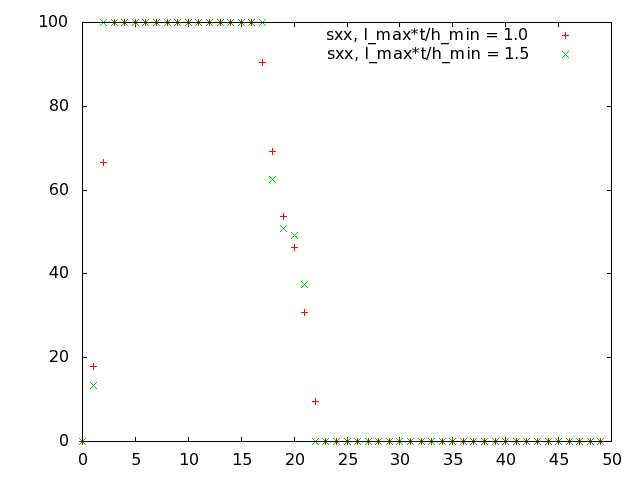
\includegraphics[width=0.8\textwidth]{png/big-sigma-test-results-1d/snap-1.png}
\caption{1-ый шаг по времени.}
\end{subfigure}
\begin{subfigure}[b]{0.5\textwidth}
\centering
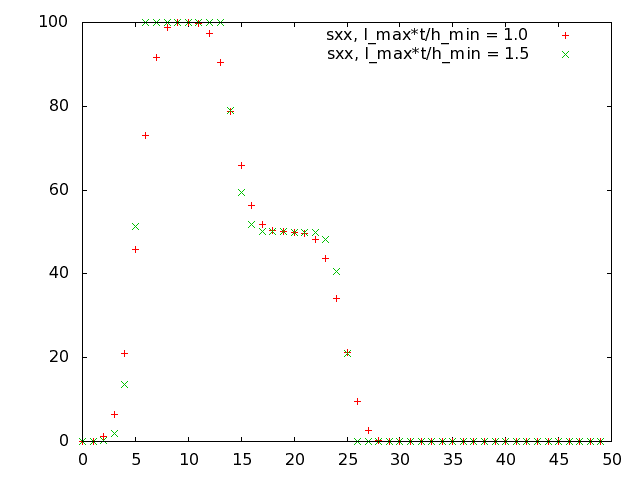
\includegraphics[width=0.8\textwidth]{png/big-sigma-test-results-1d/snap-3.png}
\caption{3-ий шаг по времени.}
\end{subfigure}
\begin{subfigure}[b]{0.5\textwidth}
\centering
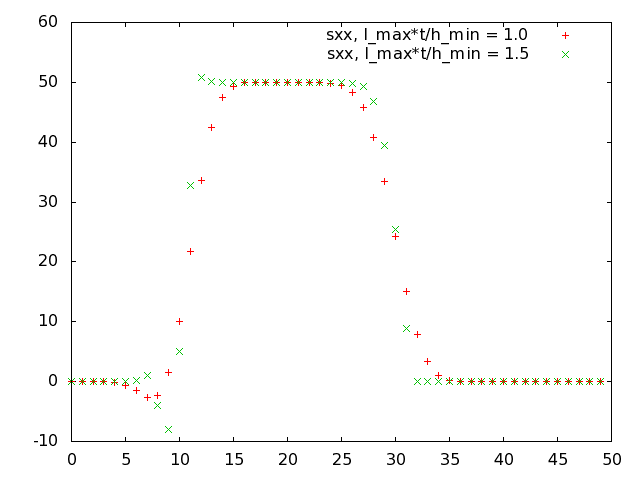
\includegraphics[width=0.8\textwidth]{png/big-sigma-test-results-1d/snap-6.png}
\caption{6-ой шаг по времени.}
\end{subfigure}
\begin{subfigure}[b]{0.5\textwidth}
\centering
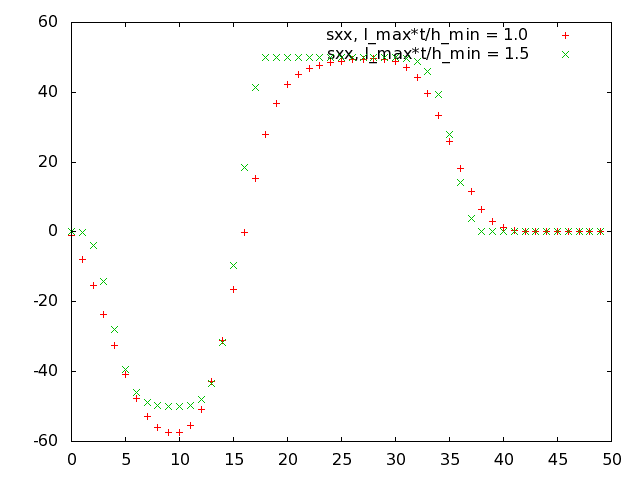
\includegraphics[width=0.8\textwidth]{png/big-sigma-test-results-1d/snap-9.png}
\caption{9-ый шаг по времени.}
\end{subfigure}
\begin{subfigure}[b]{0.5\textwidth}
\centering
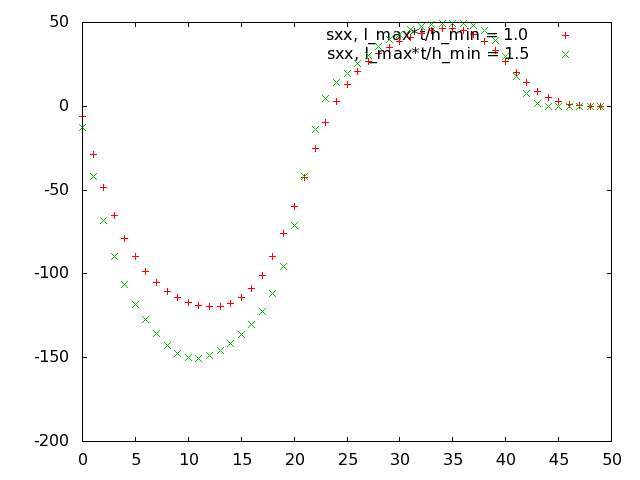
\includegraphics[width=0.8\textwidth]{png/big-sigma-test-results-1d/snap-12.png}
\caption{12-ый шаг по времени.}
\end{subfigure}
\begin{subfigure}[b]{0.5\textwidth}
\centering
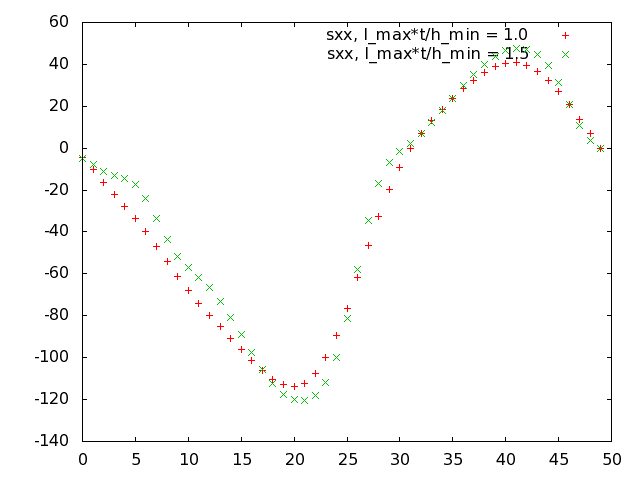
\includegraphics[width=0.8\textwidth]{png/big-sigma-test-results-1d/snap-15.png}
\caption{15-ый шаг по времени.}
\end{subfigure}
\caption{Тестирование одномерной схемы с шагом $\lambda \tau / h = 1.5$.}
\label{pic:scheme_1d_test}
\end{figure}


\subsubsection{Работа на неструктурированной сетке из тетраэдров}

Для решения многомерной задачи с большим шагом по времени ($\lambda \tau / h > 1$) используется описанный выше метод для одномерной задачи и схема расщепления по пространственным переменным. Схема расщепления конструируется ровно так же, как для случая с классическим курантовским шагом. Используется случайный выбор базиса для симметризации решения без излишнего увеличения вычислительной сложности задачи.

Расчёт внутренних, граничных и контактных узлов при таком подходе не вызывает проблем -- для каждой одномерной схемы находятся элементы сетки на прошлом временном слое, в которые попали характеристики. Для внутренних узлов все 9 характеристик оказываются внутри расчётной области, из соответствующих точек переносятся инварианты Римана и по ним восстанавливется решение на новом временном слое. Для граничных узлов 6 характеристик попадают внутрь области, а 3 уравнения, соответствующие выводящим характеристикам, заменяются на граничные условия. Для узлов на контактной границе решается система из 18 уравнений, записанных в двух соприкасающихся узлах, -- постановка контактных условий и расчёт полностью аналогичны описанному выше для случая с классическим курантовским шагом.

Отдельного подхода при расчёте с шагом по времени $\tau > h / \lambda$ требуют приграничные узлы. Они являются внутренними для расчётной области и должны рассчитываться по схеме для внутренних узлов -- по 9 значениям инвариантов Римана, перенесённым с прошлого временного слоя, и без привлечения граничных или контактных условий. Однако, в силу большого шага по времени, для узлов, расположенных достаточно близко к границе области, могут возникать характеристики, которые выходят за границы области на предыдущем временном слое.

В этом случае требуется переносить значения инвариантов Римана из виртуальных узлов, расположенных между временными слоями $n$ и $n+1$. Иллюстрация такой ситуации приведена на рис. \ref{pic:near_border_node}.

\begin{figure}[htp]
\centering
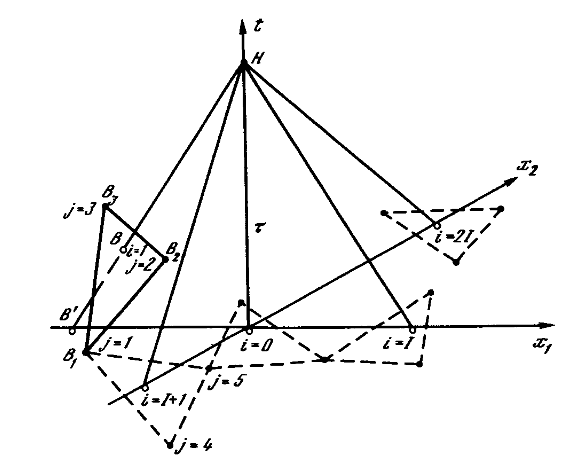
\includegraphics[width=0.6\textwidth]{png/characteristics-2d-triangles-semi-border.png}
\caption{Расчет узла, близкого к границе.}
\label{pic:near_border_node}
\end{figure}

Для одной из характеристик точка пересечения с предыдущим временным слоем оказалась за границей области интегрирования (точка $B'$). В этом случае значение переносится из точки $B$, значение в которой интерполируется по точкам $B_1, B_2, B_3$, причем точки $B_1$ и $B_2$ находятся на старом временном слое, а точка $B_3$ -- на новом. Очевидно, что при таком подходе при реализации метода требуется предусмотреть в алгоритме расчёта последовательность вычисления значений на новом временном слое -- сначала вычисляются значения в граничных узлах, после чего начинается расчёт внутренних точек.


\subsubsection{Движение сетки при больших деформациях}

Одной из традиционных проблем при расчёте задач с конечными деформациями является вырождение шага по времени из-за искажения ячеек расчётной сетки. Традиционный подход к решению этой проблемы -- перестройка сетки при появлении деформаций, переинтерполяция на новую сетку и продолжение счёта на новой сетке.

Предложенный метод расчёта с $\tau > h / \lambda$ позволяет предложить альтернативный подход к решению данной проблемы -- при искажении ячеек расчётной сетки просто продолжается счёт с прежним шагом по времени, для искажённых ячеек сетки соотношение $\lambda \tau / h$ может принимать достаточно большие значения, что обрабатывается внутренней логикой метода.

Все выполненные в рамках данной работы расчёты используют именно такой подход.


\clearpage
\newpage
\section{Характеристический метод для сеток плохого качества}

\subsection{Необходимость разработки метода}

Одной из принципиальных проблем, с которыми сталкивается метод характеристик на сетках из тетраэдров при попытке расчета им реальных задач, является низкое качество сеток, создаваемых стандартными генераторами сеток. Данный вопрос практически всегда остается за рамками в любых публикациях по теме сеточно-характеристических методов, так как не связан непосредственно с конструированием самого метода. Тем не менее, для практики эта проблема крайне важна, поэтому остановимся на ней подробнее.

Если подходить к вопросу формально, то сеточно-характеристический метод может использоваться на любой сетке из тетраэдров. Однако, как было рассмотрено выше, для сеток из тетраэдров имеет место ограничение на шаг по времени, аналогичное курантовскому шагу для равномерной прямоугольной сетки. Так для каждого узла сетки:

\begin{equation}
\tau \le \frac{\min(h)}{\max(|\lambda|)},
\end{equation}

где $\min(h)$ -- минимальная высота тетраэдра, в которые входит данный узел, $\max(|\lambda|)$ -- максимальное по модулю собственное число матрицы $\mathbf A$ для данного узла.

С практической точки зрения крайне нежелательна ситуация, когда $\tau$ оказывается малым для отдельных узлов сетки, так как это накладывает ограничения на шаг по времени для всей сетки. Разумеется, необходимо различать случай, когда малый шаг по времени продиктован объективными требованиями высокого разрешения по времени и пространству, и случай, когда он является нежелательным следствием тех или иных проблем. В данный момент мы сосредоточимся на втором случае.

В таблице \ref{tbl:mesh-stats-summary} приведены данные по сеткам из тетраэдров, созданных в кубе с ребром 10 с помощью различных генераторов. Во всех случаях было задано значение мелкости сетки $h_* = 0.25$. В идеальном случае была бы построена сетка из правильных тетраэдров одинакового размера с высотами ровно равными $h_*$. Если такое оказалось бы возможно, то шаг по времени точно соответствовал бы ожидаемому $\tau_* \le h_* / \lambda$ и зависел бы только от реологии среды (значения $\lambda$). Очевидно, что в случае реальной геометрии построить сетку полностью из правильных тетраэдров одного размера невозможно, поэтому следует ожидать появления тетраэров размером несколько больше или меньше, чем заданный, а также тетраэдров с искажениями относительно правильной формы. Полученная в итоге минимальная высота тетраэдра определяет шаг по времени для всей сетки $\tau \le \min(h) / \lambda$. В связи с этим логично ввести критерий качества сетки в следующем виде:

\begin{equation}
q = \frac{\min(h)}{h_*},
\end{equation}

где $h_*$ -- заданная желаемая мелкость сетки, а $\min(h)$ -- минимальная высота в сетке, фактически выданной генератором.

Для идеальной сетки $q = 1$. В случае не слишком больших отклонений от единицы сетку можно считать "достаточно хорошей" для расчёта. Однако, как видно из \ref{tbl:mesh-stats-summary}, на практике даже для простейшей геометрии $q$ находится в диапазоне $0.00065 \le q \le 0.126$. Это приводит к неоправданному падению шага по времени на 1-3 порядка и, соответственно, к необоснованному росту требуемого объема вычислений также на 1-3 порядка. Приведенные гистограммы распределения высот тетраэдров в полученных сетках показывают, что проблема не связана с наличием единичных вырожденных тетраэдров, а носит систематический характер. Эксперименты с объектами более сложной геометрии показывают еще худшие результаты по качеству сетки.

Причиной такого низкого качества сеток является тот факт, что все существующие генераторы сеток ориентированы на построение сеток для метода конечных элементов. Для МКЭ критерии качества сетки совершенно иные -- размеры тетраэдров не важны, для эффективной работы метода требуется, чтобы их углы были максимально близки к правильным, а линейные размеры при этом могут быть любыми. Соответственно, ориентированные на МКЭ алгоритмы построения сеток оказываются неэффективными с точки зрения сеточно-характеристического метода.

Очевидным способом решения данной проблемы может быть разработка алгоритмов построения сеток, ориентированных на улучшения качества в терминах сеточно-характеристического метода. Однако в данной работе предлагается другой подход -- модификация метода для обеспечения эффективной работы на сетке низкого качества. Данный подход, как будет рассмотрено ниже, может применяться не только для решения проблемы малого шага по времени из-за низкого качества изначальной сетки, но и в случае деградации шага по времени из-за вырождения сетки в зоне больших деформаций.

\begin{table}[h]
\centering
\begin{tabular}{|c|c|c|c|}
\hline
Генератор & Заданное $H$ & Полученное $\min(H)$ & Полученное $\max(H)$ \\
\hline
gmsh & 0.25 & 0.000845531 & 0.307492 \\
tetgen & 0.25 & 0.0315793 & 0.279029 \\
Ani3D & 0.25 & $1.08e^{-8}$ & 3.63429 \\
Ani3D + косметика & 0.25 & 0.000162557 & 3.7205 \\
\hline
\end{tabular}
\caption{Качество сеток, созданных различными генераторами в кубе с ребром 10.}
\label{tbl:mesh-stats-summary}
\end{table}


\begin{figure}[htp]
\centering
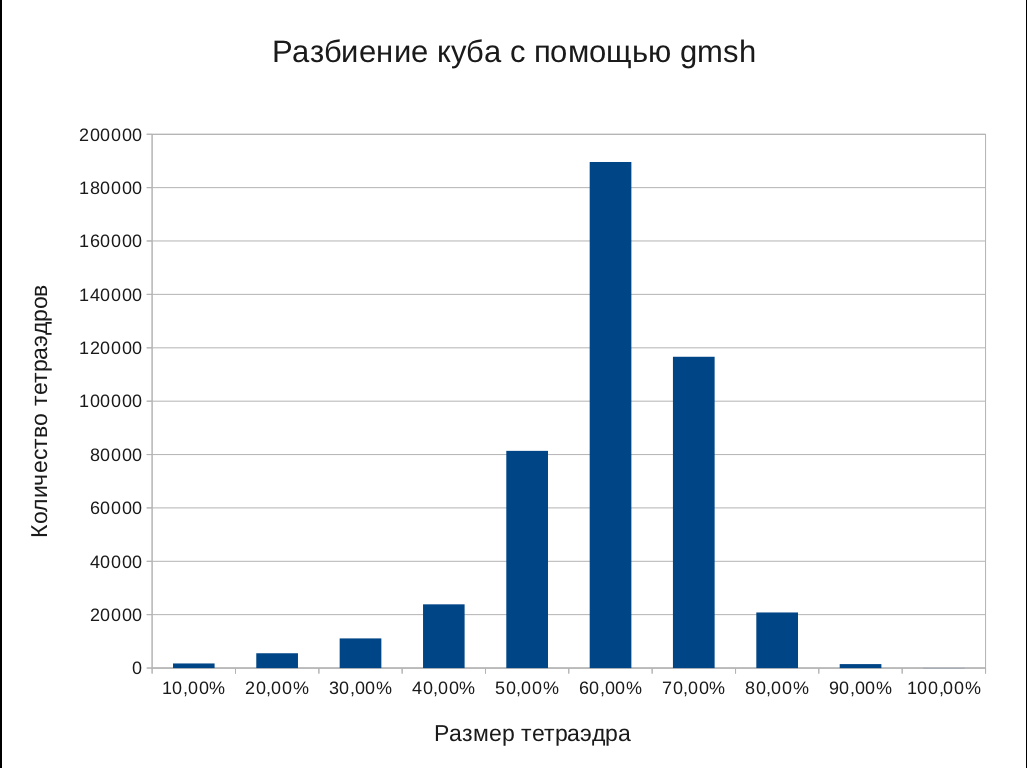
\includegraphics[width=0.8\textwidth]{png/gmsh-stats.png}
\caption{Сетка в кубе, созданная с помощью gmsh. Распределение тетраэдров по размеру.}
\end{figure}

\begin{figure}[htp]
\centering
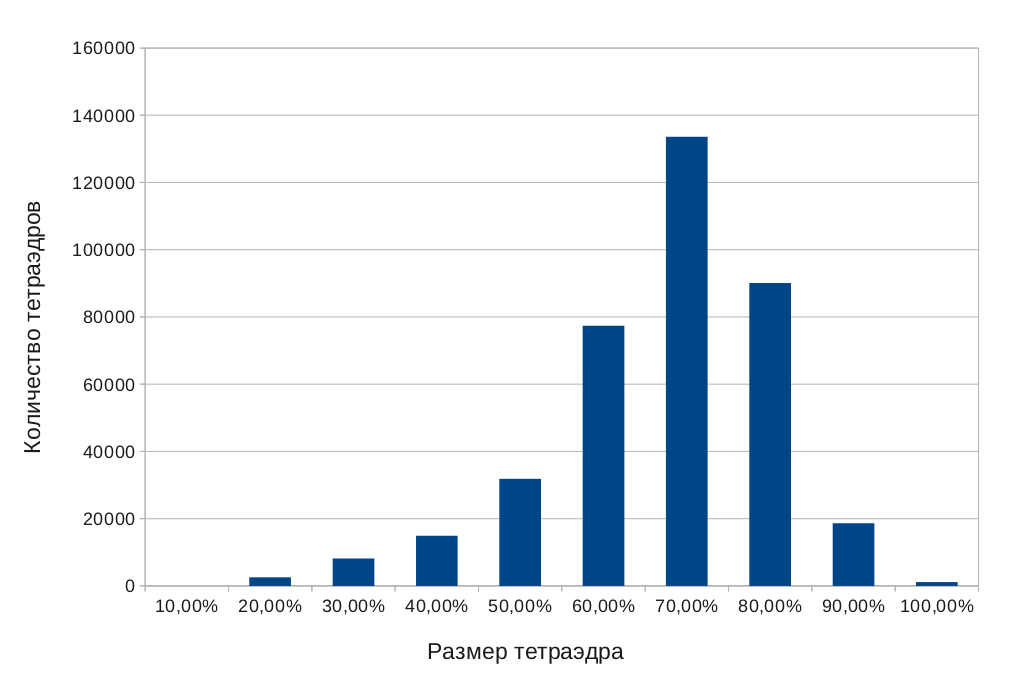
\includegraphics[width=0.8\textwidth]{png/tetgen-stats.png}
\caption{Сетка в кубе, созданная с помощью tetgen. Распределение тетраэдров по размеру.}
\end{figure}

\begin{figure}[htp]
\centering
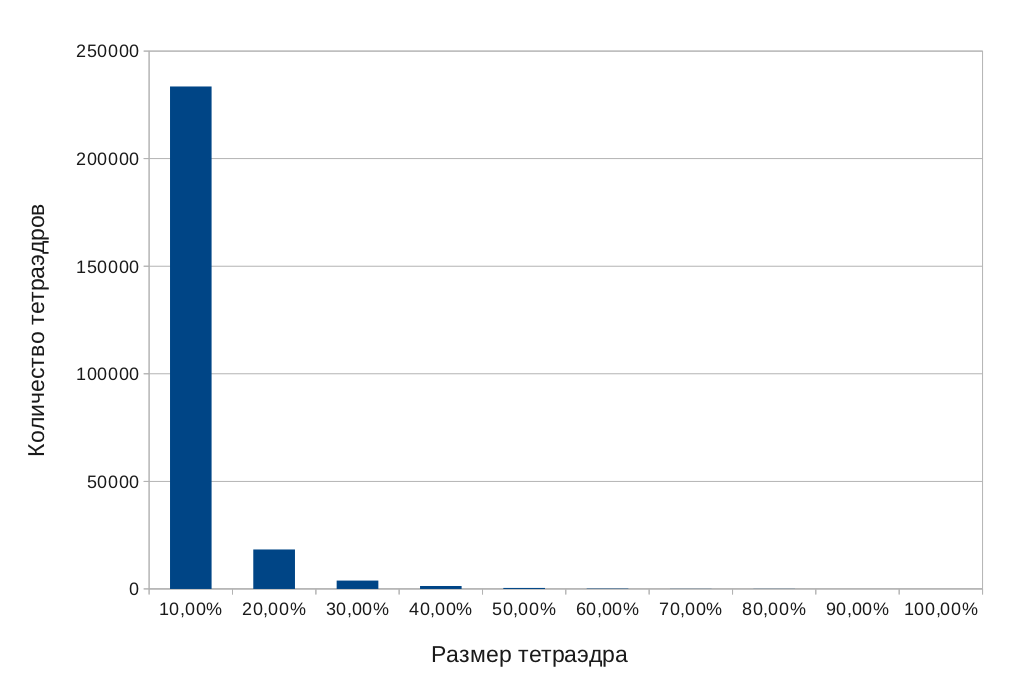
\includegraphics[width=0.8\textwidth]{png/ani3d-stats.png}
\caption{Сетка в кубе, созданная с помощью Ani3D. Распределение тетраэдров по размеру.}
\end{figure}

\begin{figure}[htp]
\centering
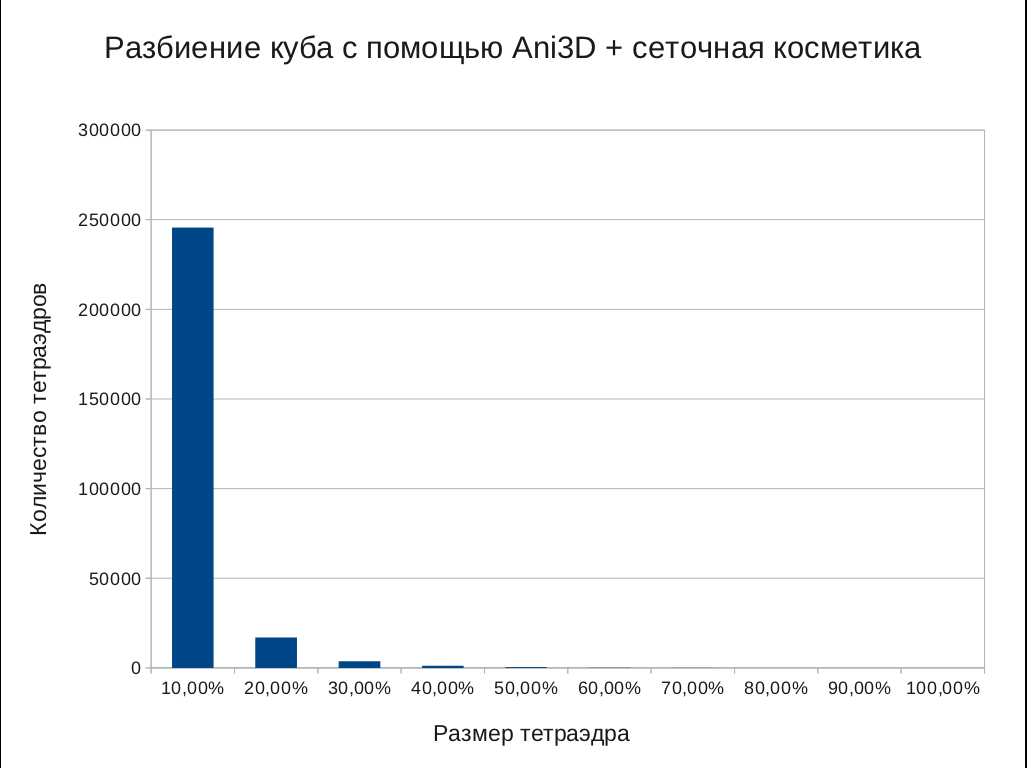
\includegraphics[width=0.8\textwidth]{png/ani3d-improved-stats.png}
\caption{Сетка в кубе, созданная с помощью Ani3D с применением сеточной косметики. Распределение тетраэдров по размеру.}
\end{figure}

\clearpage
\newpage

\subsection{Метод для одномерной задачи}

\subsubsection{Конструирование метода}

Рассмотрим одномерное уравнение переноса

\begin{equation}
\frac{\partial{u}}{\partial{t}} + \lambda \frac{\partial{u}}{\partial{x}} = 0, \lambda \ne const.
\end{equation}

Введем в области интегрирования разностную сетку и обозначим $u_m^n = u(t^n, x_m)$. Обратим внимание, что мы изначально предполагаем неравномерность сетки. Это соответствует как случаю с изначально сеткой низкого качества, так и случаю больших деформаций и вырождения сетки. Кроме того, мы рассматриваем случай разных значений $\lambda$ в разных точках расчетной области. Такая ситуация имеет место, если среда изначально неоднородная или если большие деформации вызвали значительное локальное изменение плотности в точке.

Особенностью предлагаемого метода является тот факт, что на данном этапе не будем выбирать фиксированный сеточный шаблон. Необходимые точки на предыдущем временном слое, по которым выполняется реконструкция значений на следующем шаге по времени, будут определяться в ходе вычислений отдельно для каждой рассчитываемой точки, исходя из локальных свойств решения в ней.

Предположим, что из тех или иных соображений был выбран шаг по времени $\tau$, такой что характеристика из точки $u_m^n$ не попадает в отрезок $(u_{m-1}^n; u_{m+1}^n)$.

\begin{figure}[h]
\center{\includegraphics[width=0.5\textwidth]{eps/gcm-idea.eps}}
\caption{Характеристика при большом шаге $\tau$.}
\end{figure}

В этом случае найдем тот отрезок $(u_{m-k-1}^n; u_{m-k}^n)$, в котором выпущенная характеристика пересекает временной слой $n$ (точка $x^*$ на рисунке). Обозначим:
\begin{eqnarray}
x_{m-k} - x_{m-k-1} = h_k,\nonumber\\
x_m - x^* = \lambda \tau = l_0,\nonumber\\
x_m - x_{m-k} = l_k.
\end{eqnarray}

Нормируя $l_k$ и $l_0$ на $h_k$ получаем:
\begin{eqnarray}
q_0 = l_0 / h_k = \lambda \tau / h_k = \sigma,\nonumber\\
q_k = l_k / h_k,
\end{eqnarray}
где $\sigma$ -- аналог классического числа Куранта для равномерной сетки.

Рассмотрим простейший случай линейной интерполяции значения в точке $u_*^n$ по точкам  $u_{m-k-1}^n$ и $u_{m-k}^n$. Получаем для значения на новом временном слое $u_m^{n+1}$ следующее выражение:
\begin{eqnarray}
\label{newmethod_1d_scheme}
u_m^{n+1} = u_*^n = (q_k + 1 - q_0) u_{m-k}^n + (q_0 - q_k) u_{m-k-1}^n.
\end{eqnarray}

\clearpage
\newpage

\subsubsection{Исследование метода}

Чтобы найти порядок аппроксимации по времени и по пространству используем разложение $u_{m+\mu}^{n+\nu}$ в ряд Тейлора. Обозначим:
\begin{eqnarray}
q_0 - q_k = \sigma_k,\nonumber\\
\frac{h_k}{l_0} = \alpha,\nonumber\\
\frac{l_k}{l_0} = \beta,
\end{eqnarray}
где очевидно $\alpha < 1, \beta < 1$.

Раскладывая \ref{newmethod_1d_scheme} в ряд Тейлора в окрестности $u = u_m^n$ до второго порядка малости получаем:
\begin{eqnarray}
u + u_\tau \tau + u_{\tau\tau} \frac{\tau^2}{2} = (1 - \sigma_k) (u - l_k u_x + u_{xx} \frac{l_k^2}{2}) + \sigma_k (u - (l_k+h_k) u_x + u_{xx} \frac{(l_k+h_k)^2}{2}) \nonumber\\
u_\tau \tau + u_{\tau\tau} \frac{\tau^2}{2} = (1 - \sigma_k) (- l_k u_x + u_{xx} \frac{l_k^2}{2}) + \sigma_k (- (l_k+h_k) u_x + u_{xx} \frac{(l_k+h_k)^2}{2}) \nonumber\\
u_\tau \tau + u_{\tau\tau} \frac{\tau^2}{2} = - u_x ( (1 - \sigma_k) l_k + \sigma_k (l_k+h_k) ) + \frac{u_{xx}}{2} ( (1 - \sigma_k) l_k^2 + \sigma_k (l_k+h_k)^2 ) \nonumber\\
u_\tau \tau + u_x  ( l_0 ) = - u_{\tau\tau} \frac{\tau^2}{2} + \frac{u_{xx}}{2} ( l_k^2 + 2 \sigma_k l_k h_k + \sigma_k h_k^2 ) \nonumber\\
u_\tau \tau + u_x  \lambda \tau = - u_{\tau\tau} \frac{\tau^2}{2} + \frac{u_{xx}}{2} ( l_k (l_k + \sigma_k h_k) + \sigma_k h_k (l_k + h_k) ) \nonumber\\
u_\tau \tau + u_x  \lambda \tau = - u_{\tau\tau} \frac{\tau^2}{2} + \frac{u_{xx}}{2} ( l_k l_0  + \sigma_k h_k l_0 (\alpha + \beta) ) \nonumber\\
u_\tau + u_x  \lambda = - u_{\tau\tau} \frac{\tau}{2} + \frac{u_{xx}}{2} \lambda ( l_k  + \sigma_k h_k (\alpha + \beta) ) \nonumber\\
u_\tau + u_x  \lambda = O(\tau) + O (h)
\end{eqnarray}

Таким образом, схема имеет первый порядок по времени и по пространству. Этого следовало ожидать, так как используемая линейная интерполяция имеет первый порядок точности.

Для исследования устойчивости воспользуемся методом Фурье. Рассмотрим $u_m^n = v^n e^{im\phi}$. Подставив его в \ref{newmethod_1d_scheme} получим:
\begin{eqnarray}
v^{n+1} e^{im\phi} = (q_k + 1 - q_0) v^{n} e^{i(m-k)\phi} + (q_0 - q_k) v^{n} e^{i(m-k-1)\phi} \nonumber\\
v^{n+1} e^{im\phi} = v^{n} e^{im\phi} ((q_k + 1 - q_0) e^{-ik\phi} + (q_0 - q_k) e^{-i(k+1)\phi} \nonumber\\
u_m^{n+1} = u_m^n ((q_k + 1 - q_0) e^{-ik\phi} + (q_0 - q_k) e^{-i(k+1)\phi}).
\end{eqnarray}

Таким образом, оператор перехода от слоя $n$ к слою $n+1$ имеет вид:
\begin{eqnarray}
\lambda = e^{-ik\phi} ( 1 + (q_k - q_0) (1 - e^{-i\phi}) ).
\end{eqnarray}

Необходимое условие устойчивости Неймана:
\begin{eqnarray}
|\lambda|^2 \le 1 \nonumber\\
| 1 + (q_k - q_0) (1 - e^{-i\phi}) |^2 \le 1 \nonumber\\
| 1 + (q_k - q_0) (1 - \cos(\phi)) + i(q_k - q_0)\sin(\phi) |^2 \le 1 \nonumber\\
( 1 + (q_k - q_0) (1 - \cos(\phi)))^2 + ((q_k - q_0)\sin(\phi))^2 \le 1 \nonumber\\
( 1 + q_k - q_0)^2 - 2 ( 1 + q_k - q_0)(q_k - q_0) \cos(\phi) + (q_k - q_0)^2 \le 1 \nonumber\\
1 + 2 (q_k - q_0) + 2 (q_k - q_0)^2 - 2 ( 1 + q_k - q_0)(q_k - q_0) \cos(\phi) \le 1 \nonumber\\
(q_k - q_0)^2 - (q_k - q_0) ( 1 + q_k - q_0 ) \cos(\phi) + (q_k - q_0) \le 0 \nonumber\\
(q_k - q_0)(q_k - q_0 + 1)(1 - \cos(\phi)) \le 0 \nonumber\\
(q_k - q_0)(q_k - q_0 + 1) \le 0
\end{eqnarray}

Отсюда получаем
\begin{eqnarray}
-1 \le q_k - q_0 \le 0, \nonumber\\
q_k \le q_0 \le q_k + 1.
\end{eqnarray}

Таким образом, схема устойчива при 
\begin{eqnarray}
k \le \sigma \le k+1.
\end{eqnarray}

Так как все коэффициенты схемы неотрицательны, то она также является монотонной в соответствии с критерием Фридрихса.

Полученное условие де-факто эквивалентно условию попадания характеристики в отрезок, по которому производится интерполяция. Если для реконструкции решения используется интерполяция более высоких порядков, то необходимый сеточный шаблон будет расширяться. Например, для интерполяции второго порядка необходимо использовать три точки на временном слое $n$. В этом случае можно выбрать любой из трехточечных шаблонов, включающих в себя $x^*$ -- $(u_{m-k-2}^n; u_{m-k}^n)$ или $(u_{m-k-1}^n; u_{m-k+1}^n)$. В общем случае, в соответствии с \cite{magomedov}, все схемы с порядком аппроксимации выше первого не будут монотонны.

\clearpage
\newpage

\subsubsection{Тестирование метода}

На рис. \todo{N} приведены результаты тестирования описанной схемы. Рассматривалась задача распада разрыва. Использовалась равномерная сетка по пространству. Приведены графики для расчетов с $\lambda \tau / h = 1.0$ (классический шаблон "уголок" с курантовским шагом) и $\lambda \tau / h = 1.5$ (описанная выше схема).

\begin{figure}[htp]
\centering
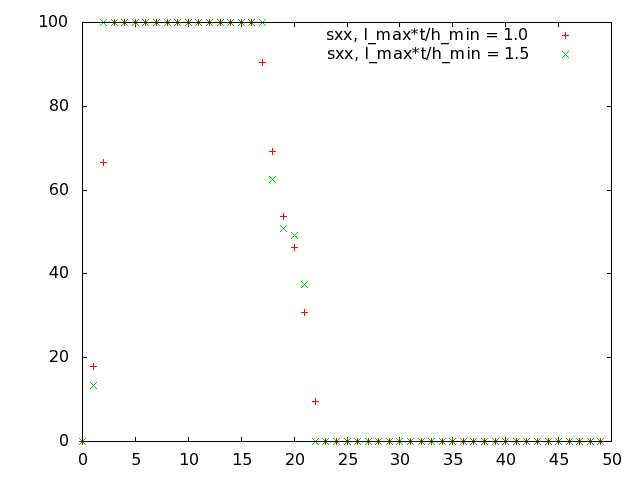
\includegraphics[width=0.6\textwidth]{png/big-sigma-test-results-1d/snap-1.png}
\caption{1-ый шаг по времени.}
\end{figure}

\begin{figure}[htp]
\centering
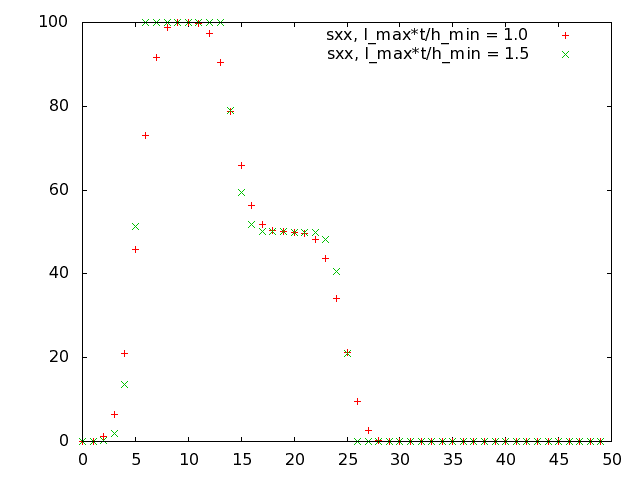
\includegraphics[width=0.6\textwidth]{png/big-sigma-test-results-1d/snap-3.png}
\caption{3-ий шаг по времени.}
\end{figure}

\begin{figure}[htp]
\centering
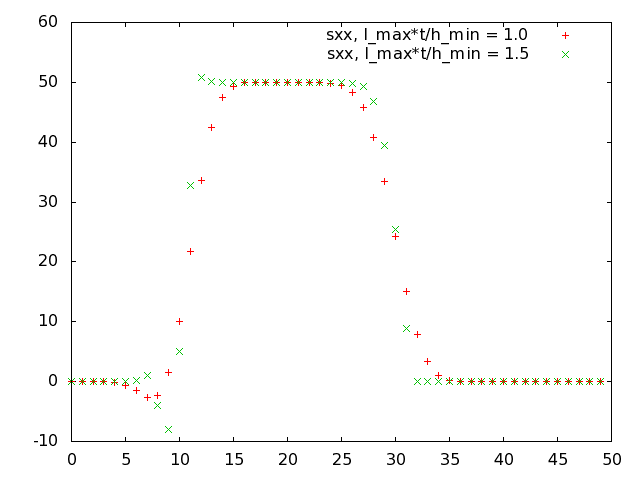
\includegraphics[width=0.6\textwidth]{png/big-sigma-test-results-1d/snap-6.png}
\caption{6-ой шаг по времени.}
\end{figure}

\begin{figure}[htp]
\centering
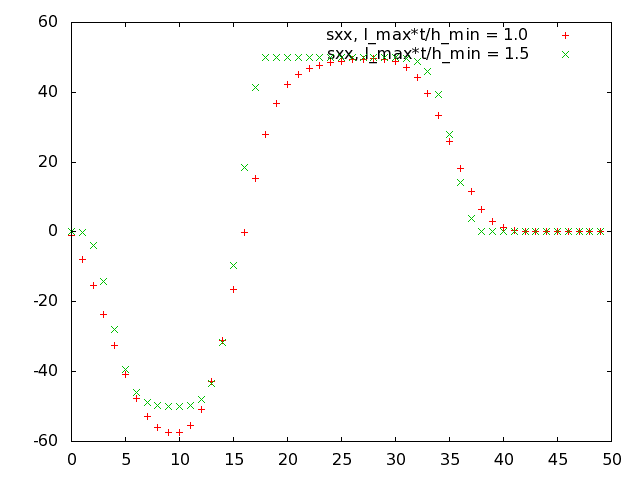
\includegraphics[width=0.6\textwidth]{png/big-sigma-test-results-1d/snap-9.png}
\caption{9-ый шаг по времени.}
\end{figure}

\begin{figure}[htp]
\centering
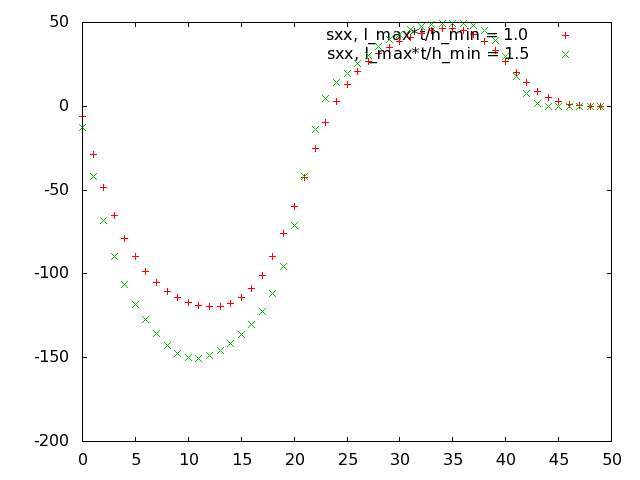
\includegraphics[width=0.6\textwidth]{png/big-sigma-test-results-1d/snap-12.png}
\caption{12-ый шаг по времени.}
\end{figure}

\clearpage
\newpage

\subsection{Метод для трёхмерной задачи}

\subsubsection{Конструирование метода на неструктурированной сетке}

\begin{figure}[htp]
\centering
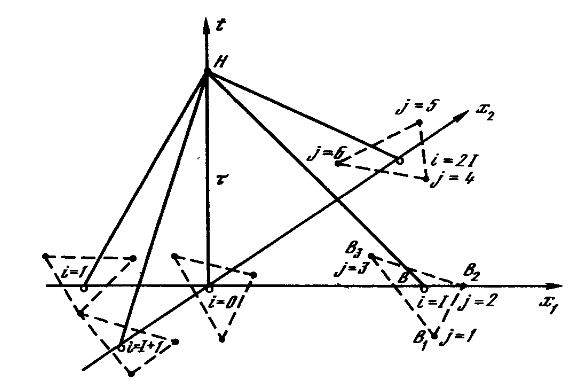
\includegraphics[width=0.6\textwidth]{png/characteristics-2d-triangles-inner.png}
\caption{Расчет внутреннего узла.}
\end{figure}

\subsubsection{Расчёт внутренних узлов}

\todo{Расчёт приграничных узлов и грабли при этом. Вылетание части характеристик.}

\begin{figure}[htp]
\centering
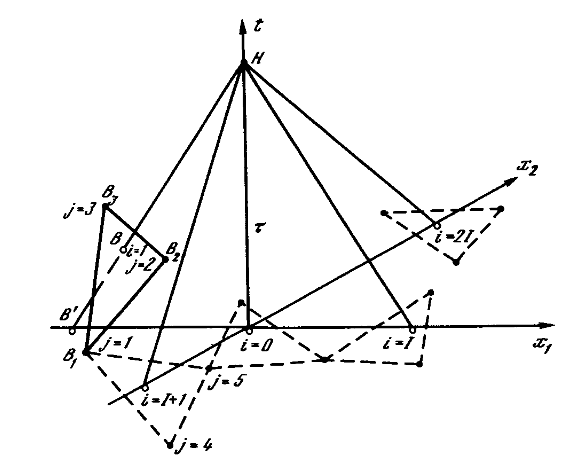
\includegraphics[width=0.6\textwidth]{png/characteristics-2d-triangles-semi-border.png}
\caption{Расчет узла, близкого к границе.}
\end{figure}


\subsubsection{Расчёт граничных и контактных узлов}

\begin{figure}[htp]
\centering
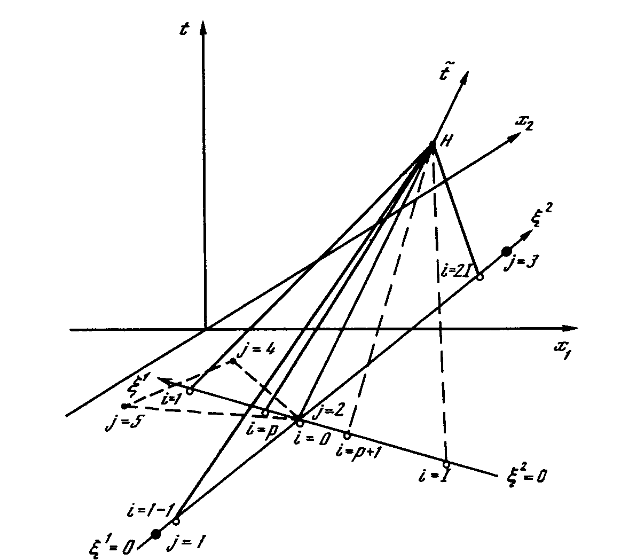
\includegraphics[width=0.6\textwidth]{png/characteristics-2d-triangles-border.png}
\caption{Расчет граничного узла.}
\end{figure}

\clearpage
\newpage

\subsubsection{Использование совместно с движущейся сеткой при больших деформациях}

\clearpage
\newpage

\subsubsection{Исследование метода}

\todo{Аппроксимация, устойчивость, монотонность}

\clearpage
\newpage

\subsubsection{Тестирование метода}

\paragraph{Распространение продольной волны (P-волны)}
Пусть плоская P-волна в среде распространяется вдоль оси z. В этом случае аналитическое решение соответствующего одномерного уравнения дает следующие соотношения на параметры волны:
\begin{itemize}
\item $v_z=-f(z)\sqrt{\frac{\lambda+2\mu}{\rho}}=C_p$;
\item $v_x=v_y=0$;
\item $\sigma_{zz}=f(z)(\lambda+2\mu)$;
\item $\sigma_{xx}=\sigma_{yy}=f(z)\lambda$;
\item $\sigma_{ij}=0$ для $i \neq j$.
\end{itemize}
Здесь $f(z)$ - произвольная функция, зависящая только от z и задающая форму волны.
Для расчёта распространения P-волны в кубе были использованы следующие безразмерные параметры: 
\begin{itemize}
\item размер расчётной области: 50x50x50;
\item $\lambda=70000$;
\item $\mu=10000$;
\item $\rho=1$.
\end{itemize}
На графиках (см. рис.
\ref{pic:p_wave_2}-\ref{pic:p_wave_22}) представлены результаты численного расчёта. Получено совпадение параметров волны с аналитическим решением:
\begin{itemize}
\item $v_z=C_p=300$;
\item $\frac{\sigma_{zz}}{\sigma_{xx}}=\frac{\sigma_{zz}}{\sigma_{yy}}=\frac{\lambda+2\mu}{\lambda}=\frac{9}{7}$.
\end{itemize}
\begin{figure}[htp]
\centering
\includegraphics[width=0.8\textwidth]{png/p-wave-propogation-3d-002.png}
\caption{Распространение P-волны, 2-й временной слой. Слева изображены
напряжения в срезе, перпендикулярном оси x, справа компоненты тензора напряжений
и модуль скорости соответственно.}
\label{pic:p_wave_2}
\end{figure}
\begin{figure}[htp]
\centering
\includegraphics[width=0.8\textwidth]{png/p-wave-propogation-3d-012.png}
\caption{Распространение P-волны, 12-й временной слой. Слева изображены
напряжения в срезе, перпендикулярном оси x, справа компоненты тензора напряжений
и модуль скорости соответственно.}
\label{pic:p_wave_12}
\end{figure}
\begin{figure}[htp]
\centering
\includegraphics[width=0.8\textwidth]{png/p-wave-propogation-3d-022.png}
\caption{Распространение P-волны, 22-й временной слой. Слева изображены
напряжения в срезе, перпендикулярном оси x, справа компоненты тензора напряжений
и модуль скорости соответственно.}
\label{pic:p_wave_22}
\end{figure}

\clearpage
\newpage

\paragraph{Распространение поперечной волны (S-волны)}
Пусть плоская S-волна в среде распространяется вдоль оси z. В этом случае аналитическое решение соответствующего одномерного уравнения дает следующие соотношения на параметры волны:
\begin{itemize}
\item $v_z=-f(z)\sqrt{\frac{\mu}{\rho}}=C_s$;
\item $v_x=v_y=0$;
\item $\sigma_{ij}=f(z)\mu$; для одной из пар $i \neq j$
\item $\sigma_{ij}=0$ для $i = j$.
\end{itemize}
Здесь $f(z)$ - произвольная функция, зависящая только от z и задающая форму волны.
Для расчёта распространения S-волны в кубе были использованы следующие безразмерные параметры: 
\begin{itemize}
\item размер расчётной области: 50x50x50;
\item $\lambda=70000$;
\item $\mu=10000$;
\item $\rho=1$.
\end{itemize}
На графиках (см. рис.
\ref{pic:s_wave_2}-\ref{pic:s_wave_22}) представлены результаты численного расчёта. Получено совпадение скорости волны с аналитическим решением:
\begin{itemize}
\item $v_z=C_s=100$.
\end{itemize}
\begin{figure}[htp]
\centering
\includegraphics[width=\textwidth]{png/s-wave-propogation-3d-002.png}
\caption{Распространение S-волны, 2-й временной слой. Слева изображены
напряжения в срезе, перпендикулярном оси x, справа компоненты тензора напряжений
и модуль скорости соответственно.}
\label{pic:s_wave_2}
\end{figure}
\begin{figure}[htp]
\centering
\includegraphics[width=\textwidth]{png/s-wave-propogation-3d-012.png}
\caption{Распространение S-волны, 12-й временной слой. Слева изображены
напряжения в срезе, перпендикулярном оси x, справа компоненты тензора напряжений
и модуль скорости соответственно.}
\label{pic:s_wave_12}
\end{figure}
\begin{figure}[htp]
\centering
\includegraphics[width=\textwidth]{png/s-wave-propogation-3d-022.png}
\caption{Распространение S-волны, 22-й временной слой. Слева изображены
напряжения в срезе, перпендикулярном оси x, справа компоненты тензора напряжений
и модуль скорости соответственно.}
\label{pic:s_wave_22}
\end{figure}

\clearpage
\newpage

\paragraph{Сферический взрыв}
Для проверки корректности расчёта при отражении от границ был произведён расчёт
модельной задачи о сферическом взрыве со следующими параметрами:
\begin{itemize}
\item размер расчётной области: 50x50x50;
\item $\lambda=70000$;
\item $\mu=10000$;
\item $\rho=1$.
\end{itemize}
На графиках (см. рис. \ref{pic:spherical_25}, \ref{pic:spherical_50}) изображены
результаты расчётов.
\begin{figure}[htp]
\begin{subfigure}[b]{0.5\textwidth}
\centering
\includegraphics[width=\textwidth]{png/v-scalar-0025.png}
\caption{Модули скоростей}
\end{subfigure}
\begin{subfigure}[b]{0.5\textwidth}
\centering
\includegraphics[width=\textwidth]{png/v-vector-0025.png}
\caption{Поле скоростей}
\end{subfigure}
\caption{Расчёт задачи о сферическом врзыве, 25-й временной-слой, волны сжатия и
растяжения. На рисунке слева цветом изображены модули скоростей в трёх взаимно
перпендикулярных плоскостях, а справа -- поле скоростей.}
\label{pic:spherical_25}
\end{figure}
\begin{figure}[htp]
\begin{subfigure}[b]{0.5\textwidth}
\centering
\includegraphics[width=\textwidth]{png/v-scalar-0050.png}
\caption{Модули скоростей}
\end{subfigure}
\begin{subfigure}[b]{0.5\textwidth}
\centering
\includegraphics[width=\textwidth]{png/v-vector-0050.png}
\caption{Поле скоростей.}
\end{subfigure}
\caption{Расчёт задачи о сферическом врзыве, 50-й временной-слой, отражение от
свободной границы. На рисунке слева цветом изображены модули скоростей в трёх взаимно
перпендикулярных плоскостях, а справа -- поле скоростей.}
\label{pic:spherical_50}
\end{figure}

%\clearpage
%\newpage
%\section{Программная реализация}

\todo{Описать полную схему в изложении для людей}

\clearpage
\newpage
\section{Построение параллельной версии}
\subsection{Необходимость}
Однопроцессорная версия алгоритма имеет весьма ограниченную применимость: основным ограничивающим фактором является объём оперативной памяти, доступной на локальном вычислительном узле. Границы применимости однопроцессорной версии можно получить при помощи следующих предположений:
\begin{itemize}
	\item используемые типы данных -- float (4 байта) и int (4 байта);
	\item в каждом узле сетки хранится 3 значения вектора скорости, 6 значений тензора, по 3 значения координат в локальной и подвижной системах, 4 значения параметров реологии среды;
	\item в процессе расчёта каждого временного шага требуется хранить копию расчётов предыдущего временного слоя, для записи результатов на жёсткий диск необходима третья копия;
	\item каждый узел хранит информацию о <<локальной>> топологии сетки для быстрого доступа к соседним тетраэдрам и треугольникам (в среднем по пять значений типа int для каждого типа элементов).
\end{itemize}

Суммарно имеем следующий расход памяти на хранения одного узла — 228 байт. В этих
расчётах не учитываются расходы на хранения топологии всей сетки, ввиду
сложности проведения оценки. Таким образом получаем, что при доступном объёме
памяти в 1 Гб для одного вычислительного узла с максимальной скоростью можно
проводить расчёты на сетках с числом узлов 1-2 миллиона. Под максимальной
скоростью здесь понимается следующее: при расчёте на сетках указанного выше
размера все необходимые данные могут быть полностью помещены в оперативной
памяти, скорость доступ к которой на порядки выше скорости чтения с жёсткого
диска.

Характерный размер сетки для решаемый задачи $\sim 2\cdot 10^6$узлов (5 слоёв,
каждый из которых имеет размер 201x201x10). Стоит
отдельно отметить, что размеры этой задачи лежат на самой нижней границе
характерных размеров задач, решение которых представляет практический интерес.
Поставленную задачу уже весьма проблематично решить на одном вычислительном узле
ввиду ограниченного размера доступной для вычислений оперативной памяти.

Другой причиной необходимости создания параллельной версии алгоритма является характер роста вычислительной сложности при увеличении числа узлов сетки ($O(n^3)$). Отсюда следует, что при уменьшении характерных размеров задачи вдвое сложность вычислений возрастает в 8 раз. Очевидно, что задачи такого класса необходимо решать при помощи параллельных версий алгоритмов, чтобы обеспечить хотя бы небольшую масштабируемость.

Таким образом, создание параллельной версии алгоритма становится необходимым условием численного моделирования задач подобного рода.

\subsection{Способ построения параллельной версии}
На данный момент существуют два прицинипиально различных подхода к реализации параллельных вычислений:
\begin{itemize}
\item взаимодействие через разделяемую память (shared memory);
\item взаимодействие при помощи обмена сообщениями.
 \end{itemize}

Первый метод позволяет <<распараллелить>> алгоритм при помощи минимальных
усилий, так как не требует существенных изменений в логике расчёта. Каждый
вычислительный узел при таком подходе имеет доступ ко всей памяти, необходимой
для расчёта задачи, которая физически находится на \emph{разных} узлах. Таким
образом, при использовании разделяемой памяти пропадает необходимость
синхронизации вычислительных узлов (в смысле пересылок данных), для организации
взаимодействия используются различные механизмы захвата управления (к примеру,
семафоры или мьютексы). Недостатком такого подхода является чисто техническое
ограничение масштабируемости алгоритма: требуется вычислительный кластер с
необходимым объёмом оперативной памяти, доступной для работы в разделяемом
режиме.

Второй подход требует существенной переработки логики алгоритма, так как необходимо явным образом проводить синхронизацию вычислительных узлов. При этом каждый вычислительный узел использует только доступную локально оперативную память, а всю необходимую информацию запрашивает посредством сообщений во время выполнения. Алгоритмы, построенные по этому принципу, обладают заметно большей масштабируемостью: на данный момент многие вычислительные кластеры имеют более тысячи процессоров.

В данный момент доступ к кластерам, построенным для вычислений с использованием
разделяемой памяти, весьма ограничен, доступные же кластеры не обладают
необходимым для серьёзного расчёта числом процессоров. Поэтому в основе
параллельной версии алгоритма, описываемого в работе, лежит обмен сообщениями
между вычислительными узлами. В качестве конкретной реализации этой парадигмы
выбран протокол MPI, признанный де-факто стандартом в области
высокопроизводительных вычислений.

\subsubsection{Идеи реализации параллельной версии при помощи обмена сообщениями}
Для реализации параллельных вычислений исходная геометрия разбивается на зоны, которые распределяются между вычислительными узлами. Один узел может производить одновременный расчёт нескольких зон. Для обеспечения согласованности расчёта вычислительные узлы обмениваются необходимой информацией о значениях и топологии сеток на границах зон. Для получения максимальной эффективности при параллельном расчёте следует учитывать следующие условия:
\begin{itemize}
	\item для увеличения времени полезного использования кластера необходимо, чтобы время расчёта очередного временного слоя на каждом вычислительном узле было примерно одинаково, так как в противном случае наиболее <<быстрые>> узлы проводят некоторые время в ожидании, при этом не проводя никаких расчётов;
	\item для увеличения скорости синхронизации и расчёта контактных границ крайне желательно, чтобы зоны имели простую геометрию;
	\item граничные части сеток различных зон должны быть построены согласованно (в идеале должны совпадать топологически) для уменьшения потерь точности, связанных с интерполяцией;
	\item расчёт каждого временного слоя должен быть максимально <<параллельным>> в том смысле, что синхронизации происходят редко и согласованно, а данные передаются большими объёмами.
\end{itemize}
\subsubsection{Тестирования производительности MPI}
Для выбора правильных API для построения параллельной версии был проведён ряд тестов производительности обмена сообщениями при помощи MPI. Одним из наиболее важных вопросов, ответ на которых хотелось получить был следующий: каков оптимальный объём сообщения для пересылки? Иными словами, нужно было выяснить, при каких размерах посылаемого сообщения время, затрачиваемое на пересылку одного байта, минимально.
Ниже приведены графики (см. рис. \ref{pic:mpi1host} и рис. \ref{pic:mpi2hosts} зависимости затрат на пересылку одного байта в зависимости от размера сообщения.
\begin{figure}[htp]
\centering
\includegraphics[width=0.6\textwidth]{eps/mpi-1host.eps}
\caption{Затраты на пересылки при использовании одного вычислительного
 узла.}
\label{pic:mpi1host}
\end{figure}
\begin{figure}[htp]
\centering
\includegraphics[width=0.6\textwidth]{eps/mpi-2hosts.eps}
\caption{Затраты на пересылки при использовании двух вычислительных узлов.}
\label{pic:mpi2hosts}
\end{figure}
Как видно из графиков, для пересылки данных посредством MPI выгодно использовать
большие объёмы сообщений. В первую очередь это связано с ростом доли накладных
расходов на пересылку сообщения при уменьшении его размера. Другими факторами,
снижающими скорость передачи, могут служить буферизация исходящих сообщений, а
также блокировки вызывающего процесса при синхронной передаче данных. По
результатам проведённых тестов были сделаны следующие выводы:
\begin{itemize}
	\item данные нужно передавать большими объёмами, так как скорость в таких случаях выше;
	\item следует использовать асинхронную передачу данных, возможно, с инициацией приёма до момента посылки данных;
	\item для ускорения процесса синхронизации крайне желательно использовать <<родные>> функции коллективного обмена данными вместо самостоятельной реализации подобного функционала;
	\item следует в полной мере использовать возможности MPI по созданию пользовательских типов данных для уменьшения объёмов памяти, требуемых для хранения временных структур данных, а также для уменьшения временн\'{ы}х затрат на копирование данных внутри вычислительного узла.
\end{itemize}

\subsubsection{Синхронизация шага по времени}
Перед расчётом очередного временного слоя необходимо синхронизировать шаг по времени между всеми вычислительными узлами. В текущей реализации метода с целью увеличения скорости расчёта вводится ограничение на максимально возможный шаг по времени:
\begin{equation}
\label{max_time_step}
\tau_{max}=\frac{h_{min}}{\lambda_{max}},
\end{equation}
где $h_{min}$ -- минимальная высота тетраэдра в сетке, а $\lambda_{max}$ --
максимальное значение коэффициента Ляме в локальной сетке. Так как для расчётов
используются неструктурированные тетраэдральные сетки, максимально допустимый
шаг по времени может различаться для разных зон. Поэтому в начале расчёта
каждого временного слоя вычислительные узлы выбирают максимально допустимый шаг
по времени для локальных сеток, после чего выбирают минимальный из всех
полученных. Дальнейший расчёт на всех вычислительных узлах ведётся с одним и тем
же шагом по времени. Для выполнения этой операции крайне удобным оказалось
использовать встроенную в MPI функцию коллективного
обмена:\lstinputlisting[label=lst:time_step_sync,caption=Синхронизация шага по
времени.]{source/time_step_sync.cpp}
\subsubsection{Синхронизация узлов}
Как было сказано ранее, при параллельных вычисления исходная сетка делится между вычислительными узлами. При этом нередки ситуации, когда одно физическое тело <<разрезано>> на несколько зон. В этом случае получаем следующее: часть узлов, необходимых для расчёта сетки А, принадлежат сетке Б (см. рис. \ref{pic:remote_nodes}). Именно эти узлы (на этапе загрузки они помечаются как REMOTE) необходимо синхронизировать.
\begin{figure}[htp]
\centering
\includegraphics[width=0.4\textwidth]{eps/remote_nodes.eps}
\caption{REMOTE узлы на сетках.}
\label{pic:remote_nodes}
\end{figure}
В текущей реализации не используется динамическое перестроение сеток, поэтому на протяжении всего расчёта набор REMOTE узлов не меняется. Это позволяет на этапе загрузки провести первичную обработку сеток, получить список REMOTE узлов для каждой пары сеток и создать пользовательские типы MPI для дальнейших пересылок между вычислительными узлами. Характерный код создания пользовательских типов MPI:
\lstinputlisting[label=lst:custom_types,caption=Создание пользовательских типов
MPI.]{source/custom_types.cpp}
После этого пересылка всех узлов выполняется так:
\lstinputlisting[label=lst:nodes_sync,caption=Синхронизация REMOTE узлов.]{source/nodes_sync.cpp}
\subsubsection{Параллельный детектор столкновений}
Параллельная версия алгоритма выделения контактных границ принципиально не отличается от последовательной. На первом шаге расчёта контактных границ все вычислительные узлы синхронизируют AABB локальных зон, для чего используется вызов стандартной функции MPI:
\lstinputlisting[label=lst:outlines_sync,caption=Синхронизация AABB.]{source/outlines_sync.cpp}
После этого каждый вычислительный узел определяет пары <<потенциально>> находящихся в контакте зон -- одной локальной и одной удалённой. Затем для каждой найденной пары проводится уточнение зоны контакта: проверяются <<на контакт>> все пары локальных узлов и удалённых треугольников. Для этого проводится синхронизация треугольников, попавших в зону контакта. Идея здесь схожа с той, что используется при синхронизации удалённых узлов, но имеет некоторые отличия:
\begin{itemize}
	\item т.к. номера треугольников, попавших в зону контакта, заранее не известны, необходимо на первом шаге получить их;
	\item затем, чтобы использовать только одну пересылку на зону контакта, необходимо создать пользовательский тип MPI;
	\item последний шаг -- отправка найденных треугольников получателю.
\end{itemize}
После того, как все треугольники в зоне контакта получены с удалённого вычислительного узла, полным перебором определяются пары <<контактирующих>> узлов и треугольников, строятся виртуальные узлы и интерполируются значения в них. Эта часть алгоритма не отличается от последовательной версии.
\subsubsection{Синхронизация тетраэдров}
Синхронизация тетраэдров необходима для реконструкции локальной топологии сетки, что требуется для правильного расчёта контактной границы. Идеи реализации схожи с теми, что были описаны выше:
\begin{itemize}
	\item вычислительный узел получает список треугольников, для которых нужно синхронизировать тетраэдры;
	\item по списку треугольников строится список тетраэдров, которые необходимо передать удалённому вычислительному узлу;
	\item создаётся пользовательский тип MPI и за одну пересылку осуществляется синхронизация тетраэдров.
\end{itemize}
\subsubsection{Производительность параллельной версии}
Для измерения производительности параллельной версии алгоритма были проведены
расчёты одной и той же тестовой задачи на разном числе вычислительных узлов с
разным способом расчёта контактной границы. В
качестве тестовой задачи была взята задача о распространении волн в 24-слойной
преграде. Каждый слой представляет собой прямоугольный параллелепипед размера
120x120x5 точек. На рисунках \ref{pic:gcm_boost} и
\ref{pic:gcm_efficiency} представлены зависимости производительности и
эффективности от числа используемых вычислительных узлов.
\begin{figure}[htp]
\centering
\includegraphics[width=0.6\textwidth]{eps/gcm3d-boost.eps}
\caption{Зависимость производительности от количества вычислительных узлов.}
\label{pic:gcm_boost}
\end{figure}
\begin{figure}[htp]
\centering
\includegraphics[width=0.6\textwidth]{eps/gcm3d-efficiency.eps}
\caption{Зависимость эффективности использования кластера от количества
вычислительных узлов.}
\label{pic:gcm_efficiency}
\end{figure}

Как видно из графиков, использование сквозного счёта даёт практически линейный
рост производительности с эффективным временем использования кластера в $\sim
90\%$.
Расчёт с явным выделением контакта даёт производительность в $\sim30\%$. Это  в
первую очередь связано с очень большой площадью контактирующих поверхностей. Так, в тестовом
примере $\sim 40\%$ узлов исходной сетки принимают участие в расчёте контакта.
При этом распределение контактирующих поверхностей по вычислительным узлам
неоднородно: слои, находящиеся <<в центре>> имеют по две контактирующих
поверхности, а <<крайние>> слои лишь по одной.

Полученные характеристики производительности следует воспринимать как оценочные
для верхней и нижней границ. Соответственно, ожидаемая эффективность при расчёте
реальных задач должна составить $\sim 60\%$. Этот результат является вполне
приемлемым, так как позволяет обеспечить расчёт больших областей с высокой
точностью при разумном КПД.

\clearpage
\newpage
\section{Тестирование метода}

\subsection{Распространение продольной волны (P-волны)}
Пусть плоская P-волна в среде распространяется вдоль оси z. В этом случае аналитическое решение соответствующего одномерного уравнения дает следующие соотношения на параметры волны:
\begin{itemize}
\item $v_z=-f(z)\sqrt{\frac{\lambda+2\mu}{\rho}}=C_p$;
\item $v_x=v_y=0$;
\item $\sigma_{zz}=f(z)(\lambda+2\mu)$;
\item $\sigma_{xx}=\sigma_{yy}=f(z)\lambda$;
\item $\sigma_{ij}=0$ для $i \neq j$.
\end{itemize}
Здесь $f(z)$ - произвольная функция, зависящая только от z и задающая форму волны.
Для расчёта распространения P-волны в кубе были использованы следующие безразмерные параметры: 
\begin{itemize}
\item размер расчётной области: 50x50x50;
\item $\lambda=70000$;
\item $\mu=10000$;
\item $\rho=1$.
\end{itemize}
На графиках (см. рис.
\ref{pic:p_wave_1}-\ref{pic:p_wave_15}) представлены результаты численного расчёта. Получено совпадение параметров волны с аналитическим решением:
\begin{itemize}
\item $v_z=C_p=300$;
\item $\frac{\sigma_{zz}}{\sigma_{xx}}=\frac{\sigma_{zz}}{\sigma_{yy}}=\frac{\lambda+2\mu}{\lambda}=\frac{9}{7}$.
\end{itemize}

\begin{figure}[htp]
\centering
\includegraphics[width=0.8\textwidth]{png/p-wave-test/s/0001.png}
\caption{Распространение P-волны, 1-й временной слой. Изображены компоненты тензора напряжений.}
\label{pic:p_wave_1}
\end{figure}

\begin{figure}[htp]
\centering
\includegraphics[width=0.8\textwidth]{png/p-wave-test/s/0003.png}
\caption{Распространение P-волны, 3-й временной слой. Изображены компоненты тензора напряжений.}
\end{figure}

\begin{figure}[htp]
\centering
\includegraphics[width=0.8\textwidth]{png/p-wave-test/s/0005.png}
\caption{Распространение P-волны, 5-й временной слой. Изображены компоненты тензора напряжений.}
\end{figure}

\begin{figure}[htp]
\centering
\includegraphics[width=0.8\textwidth]{png/p-wave-test/s/0007.png}
\caption{Распространение P-волны, 7-й временной слой. Изображены компоненты тензора напряжений.}
\end{figure}

\begin{figure}[htp]
\centering
\includegraphics[width=0.8\textwidth]{png/p-wave-test/s/0009.png}
\caption{Распространение P-волны, 9-й временной слой. Изображены компоненты тензора напряжений.}
\end{figure}

\begin{figure}[htp]
\centering
\includegraphics[width=0.8\textwidth]{png/p-wave-test/s/0011.png}
\caption{Распространение P-волны, 11-й временной слой. Изображены компоненты тензора напряжений.}
\end{figure}

\begin{figure}[htp]
\centering
\includegraphics[width=0.8\textwidth]{png/p-wave-test/s/0013.png}
\caption{Распространение P-волны, 13-й временной слой. Изображены компоненты тензора напряжений.}
\end{figure}

\begin{figure}[htp]
\centering
\includegraphics[width=0.8\textwidth]{png/p-wave-test/s/0015.png}
\caption{Распространение P-волны, 15-й временной слой. Изображены компоненты тензора напряжений.}
\label{pic:p_wave_15}
\end{figure}

\clearpage
\newpage

\subsection{Распространение поперечной волны (S-волны)}
Пусть плоская S-волна в среде распространяется вдоль оси z. В этом случае аналитическое решение соответствующего одномерного уравнения дает следующие соотношения на параметры волны:
\begin{itemize}
\item $v_z=-f(z)\sqrt{\frac{\mu}{\rho}}=C_s$;
\item $v_x=v_y=0$;
\item $\sigma_{ij}=f(z)\mu$; для одной из пар $i \neq j$
\item $\sigma_{ij}=0$ для $i = j$.
\end{itemize}
Здесь $f(z)$ - произвольная функция, зависящая только от z и задающая форму волны.
Для расчёта распространения S-волны в кубе были использованы следующие безразмерные параметры: 
\begin{itemize}
\item размер расчётной области: 50x50x50;
\item $\lambda=70000$;
\item $\mu=10000$;
\item $\rho=1$.
\end{itemize}
На графиках (см. рис.
\ref{pic:s_wave_1}-\ref{pic:s_wave_15}) представлены результаты численного расчёта. Получено совпадение скорости волны с аналитическим решением:
\begin{itemize}
\item $v_z=C_s=100$.
\end{itemize}

\begin{figure}[htp]
\centering
\includegraphics[width=0.8\textwidth]{png/s-wave-test/s/0001.png}
\caption{Распространение S-волны, 1-й временной слой. Изображены компоненты тензора напряжений.}
\label{pic:s_wave_1}
\end{figure}

\begin{figure}[htp]
\centering
\includegraphics[width=0.8\textwidth]{png/s-wave-test/s/0003.png}
\caption{Распространение S-волны, 3-й временной слой. Изображены компоненты тензора напряжений.}
\end{figure}

\begin{figure}[htp]
\centering
\includegraphics[width=0.8\textwidth]{png/s-wave-test/s/0005.png}
\caption{Распространение S-волны, 5-й временной слой. Изображены компоненты тензора напряжений.}
\end{figure}

\begin{figure}[htp]
\centering
\includegraphics[width=0.8\textwidth]{png/s-wave-test/s/0007.png}
\caption{Распространение S-волны, 7-й временной слой. Изображены компоненты тензора напряжений.}
\end{figure}

\begin{figure}[htp]
\centering
\includegraphics[width=0.8\textwidth]{png/s-wave-test/s/0009.png}
\caption{Распространение S-волны, 9-й временной слой. Изображены компоненты тензора напряжений.}
\end{figure}

\begin{figure}[htp]
\centering
\includegraphics[width=0.8\textwidth]{png/s-wave-test/s/0011.png}
\caption{Распространение S-волны, 11-й временной слой. Изображены компоненты тензора напряжений.}
\end{figure}

\begin{figure}[htp]
\centering
\includegraphics[width=0.8\textwidth]{png/s-wave-test/s/0013.png}
\caption{Распространение S-волны, 13-й временной слой. Изображены компоненты тензора напряжений.}
\end{figure}

\begin{figure}[htp]
\centering
\includegraphics[width=0.8\textwidth]{png/s-wave-test/s/0015.png}
\caption{Распространение S-волны, 15-й временной слой. Изображены компоненты тензора напряжений.}
\label{pic:s_wave_15}
\end{figure}

\clearpage
\newpage

\subsection{Сферический взрыв}
Для проверки изотропии схемы и корректности расчёта при отражении от границ был произведён расчёт
модельной задачи о сферическом взрыве со следующими параметрами:
\begin{itemize}
\item размер расчётной области: 50x50x50;
\item $\lambda=70000$;
\item $\mu=10000$;
\item $\rho=1$.
\end{itemize}
На графиках (см. рис. \ref{pic:spherical_1}-\ref{pic:spherical_70}) изображены
результаты расчётов.

\begin{figure}[htp]
\centering
\includegraphics[width=0.6\textwidth]{png/spherical-explosion-test/v-scalar/0001.png}
\caption{Расчёт задачи о сферическом врзыве, 1-й временной слой. Цветом изображен модуль скоростей.}
\label{pic:spherical_1}
\end{figure}

\begin{figure}[htp]
\centering
\includegraphics[width=0.6\textwidth]{png/spherical-explosion-test/v-scalar/0005.png}
\caption{Расчёт задачи о сферическом врзыве, 5-й временной слой. Цветом изображен модуль скоростей.}
\end{figure}

\begin{figure}[htp]
\centering
\includegraphics[width=0.6\textwidth]{png/spherical-explosion-test/v-scalar/0010.png}
\caption{Расчёт задачи о сферическом врзыве, 10-й временной слой. Цветом изображен модуль скоростей.}
\end{figure}

\begin{figure}[htp]
\centering
\includegraphics[width=0.6\textwidth]{png/spherical-explosion-test/v-scalar/0015.png}
\caption{Расчёт задачи о сферическом врзыве, 15-й временной слой. Цветом изображен модуль скоростей.}
\end{figure}

\begin{figure}[htp]
\centering
\includegraphics[width=0.6\textwidth]{png/spherical-explosion-test/v-scalar/0020.png}
\caption{Расчёт задачи о сферическом врзыве, 20-й временной слой. Цветом изображен модуль скоростей.}
\end{figure}

\begin{figure}[htp]
\centering
\includegraphics[width=0.6\textwidth]{png/spherical-explosion-test/v-scalar/0025.png}
\caption{Расчёт задачи о сферическом врзыве, 25-й временной слой. Цветом изображен модуль скоростей.}
\end{figure}

\begin{figure}[htp]
\centering
\includegraphics[width=0.6\textwidth]{png/spherical-explosion-test/v-scalar/0030.png}
\caption{Расчёт задачи о сферическом врзыве, 30-й временной слой. Цветом изображен модуль скоростей.}
\end{figure}

\begin{figure}[htp]
\centering
\includegraphics[width=0.6\textwidth]{png/spherical-explosion-test/v-scalar/0035.png}
\caption{Расчёт задачи о сферическом врзыве, 35-й временной слой. Цветом изображен модуль скоростей.}
\end{figure}

\begin{figure}[htp]
\centering
\includegraphics[width=0.6\textwidth]{png/spherical-explosion-test/v-scalar/0040.png}
\caption{Расчёт задачи о сферическом врзыве, 40-й временной слой. Цветом изображен модуль скоростей.}
\end{figure}

\begin{figure}[htp]
\centering
\includegraphics[width=0.6\textwidth]{png/spherical-explosion-test/v-scalar/0045.png}
\caption{Расчёт задачи о сферическом врзыве, 45-й временной слой. Цветом изображен модуль скоростей.}
\end{figure}

\begin{figure}[htp]
\centering
\includegraphics[width=0.6\textwidth]{png/spherical-explosion-test/v-scalar/0050.png}
\caption{Расчёт задачи о сферическом врзыве, 50-й временной слой. Цветом изображен модуль скоростей.}
\end{figure}

\begin{figure}[htp]
\centering
\includegraphics[width=0.6\textwidth]{png/spherical-explosion-test/v-scalar/0055.png}
\caption{Расчёт задачи о сферическом врзыве, 55-й временной слой. Цветом изображен модуль скоростей.}
\end{figure}

\begin{figure}[htp]
\centering
\includegraphics[width=0.6\textwidth]{png/spherical-explosion-test/v-scalar/0060.png}
\caption{Расчёт задачи о сферическом врзыве, 60-й временной слой. Цветом изображен модуль скоростей.}
\end{figure}

\begin{figure}[htp]
\centering
\includegraphics[width=0.6\textwidth]{png/spherical-explosion-test/v-scalar/0065.png}
\caption{Расчёт задачи о сферическом врзыве, 65-й временной слой. Цветом изображен модуль скоростей.}
\end{figure}

\begin{figure}[htp]
\centering
\includegraphics[width=0.6\textwidth]{png/spherical-explosion-test/v-scalar/0070.png}
\caption{Расчёт задачи о сферическом врзыве, 70-й временной слой. Цветом изображен модуль скоростей.}
\label{pic:spherical_70}
\end{figure}

\clearpage
\newpage

\subsection{Конечные деформации}
Для проверки расчета при конечных деформациях был выполнен расчёт модельной задачи о воздействии ударника на пластину. Воздействие задавалось граничным условием на нормальную компоненту силы в области удара.

На графиках (см. рис. \ref{pic:moving_border_1}-\ref{pic:moving_border_40}) изображены результаты расчётов.

\begin{figure}[htp]
\centering
\includegraphics[width=0.6\textwidth]{png/border-test/v-2d/0001.png}
\caption{Расчёт задачи о вхождении ударника в пластину, 1-й временной слой. Цветом изображен модуль скоростей.}
\label{pic:moving_border_1}
\end{figure}

\begin{figure}[htp]
\centering
\includegraphics[width=0.6\textwidth]{png/border-test/v-2d/0010.png}
\caption{Расчёт задачи о вхождении ударника в пластину, 10-й временной слой. Цветом изображен модуль скоростей.}
\end{figure}

\begin{figure}[htp]
\centering
\includegraphics[width=0.6\textwidth]{png/border-test/v-2d/0020.png}
\caption{Расчёт задачи о вхождении ударника в пластину, 20-й временной слой. Цветом изображен модуль скоростей.}
\end{figure}

\begin{figure}[htp]
\centering
\includegraphics[width=0.6\textwidth]{png/border-test/v-2d/0030.png}
\caption{Расчёт задачи о вхождении ударника в пластину, 30-й временной слой. Цветом изображен модуль скоростей.}
\end{figure}

\begin{figure}[htp]
\centering
\includegraphics[width=0.6\textwidth]{png/border-test/v-2d/0040.png}
\caption{Расчёт задачи о вхождении ударника в пластину, 40-й временной слой. Цветом изображен модуль скоростей.}
\label{pic:moving_border_40}
\end{figure}


\clearpage
\newpage

\subsection{Контакт тел}
Для проверки расчета контактных границ и взаимодействия тел был выполнен расчёт задачи об ударе по пластине с явным моделированием пластины и ударника на отдельных сетках.

На графиках (см. рис. \ref{pic:striker_test_2d_1}-\ref{pic:striker_test_2d_280}) изображены поля скоростей в пластине и ударнике.

\begin{figure}[htp]
\centering
\includegraphics[width=0.6\textwidth]{png/strike-test/both-2d/0001.png}
\caption{Поля скоростей в ударнике и пластине. 1-й временной слой. Цветом изображен модуль скорости.}
\label{pic:striker_test_2d_1}
\end{figure}

\begin{figure}[htp]
\centering
\includegraphics[width=0.6\textwidth]{png/strike-test/both-2d/0040.png}
\caption{Поля скоростей в ударнике и пластине. 40-й временной слой. Цветом изображен модуль скорости.}
\end{figure}

\begin{figure}[htp]
\centering
\includegraphics[width=0.6\textwidth]{png/strike-test/both-2d/0080.png}
\caption{Поля скоростей в ударнике и пластине. 80-й временной слой. Цветом изображен модуль скорости.}
\end{figure}

\begin{figure}[htp]
\centering
\includegraphics[width=0.6\textwidth]{png/strike-test/both-2d/0120.png}
\caption{Поля скоростей в ударнике и пластине. 120-й временной слой. Цветом изображен модуль скорости.}
\end{figure}

\begin{figure}[htp]
\centering
\includegraphics[width=0.6\textwidth]{png/strike-test/both-2d/0160.png}
\caption{Поля скоростей в ударнике и пластине. 160-й временной слой. Цветом изображен модуль скорости.}
\end{figure}

\begin{figure}[htp]
\centering
\includegraphics[width=0.6\textwidth]{png/strike-test/both-2d/0200.png}
\caption{Поля скоростей в ударнике и пластине. 200-й временной слой. Цветом изображен модуль скорости.}
\end{figure}

\begin{figure}[htp]
\centering
\includegraphics[width=0.6\textwidth]{png/strike-test/both-2d/0240.png}
\caption{Поля скоростей в ударнике и пластине. 240-й временной слой. Цветом изображен модуль скорости.}
\end{figure}

\begin{figure}[htp]
\centering
\includegraphics[width=0.6\textwidth]{png/strike-test/both-2d/0280.png}
\caption{Поля скоростей в ударнике и пластине. 280-й временной слой. Цветом изображен модуль скорости.}
\label{pic:striker_test_2d_280}
\end{figure}

\clearpage

На графиках (см. рис. \ref{pic:striker_test_plate_1}-\ref{pic:striker_test_plate_200}) изображено трёхмерное распределение поля скоростей в пластине.

\begin{figure}[htp]
\centering
\includegraphics[width=0.6\textwidth]{png/strike-test/plate-3d-v/0001.png}
\caption{Трёхмерное распределение поля скоростей в пластине. 1-й временной слой. Цветом изображен модуль скорости.}
\label{pic:striker_test_plate_1}
\end{figure}

\begin{figure}[htp]
\centering
\includegraphics[width=0.6\textwidth]{png/strike-test/plate-3d-v/0020.png}
\caption{Трёхмерное распределение поля скоростей в пластине. 20-й временной слой. Цветом изображен модуль скорости.}
\end{figure}

\begin{figure}[htp]
\centering
\includegraphics[width=0.6\textwidth]{png/strike-test/plate-3d-v/0040.png}
\caption{Трёхмерное распределение поля скоростей в пластине. 40-й временной слой. Цветом изображен модуль скорости.}
\end{figure}

\begin{figure}[htp]
\centering
\includegraphics[width=0.6\textwidth]{png/strike-test/plate-3d-v/0060.png}
\caption{Трёхмерное распределение поля скоростей в пластине. 60-й временной слой. Цветом изображен модуль скорости.}
\end{figure}

\begin{figure}[htp]
\centering
\includegraphics[width=0.6\textwidth]{png/strike-test/plate-3d-v/0080.png}
\caption{Трёхмерное распределение поля скоростей в пластине. 80-й временной слой. Цветом изображен модуль скорости.}
\end{figure}

\begin{figure}[htp]
\centering
\includegraphics[width=0.6\textwidth]{png/strike-test/plate-3d-v/0100.png}
\caption{Трёхмерное распределение поля скоростей в пластине. 100-й временной слой. Цветом изображен модуль скорости.}
\end{figure}

\begin{figure}[htp]
\centering
\includegraphics[width=0.6\textwidth]{png/strike-test/plate-3d-v/0120.png}
\caption{Трёхмерное распределение поля скоростей в пластине. 120-й временной слой. Цветом изображен модуль скорости.}
\end{figure}

\begin{figure}[htp]
\centering
\includegraphics[width=0.6\textwidth]{png/strike-test/plate-3d-v/0140.png}
\caption{Трёхмерное распределение поля скоростей в пластине. 140-й временной слой. Цветом изображен модуль скорости.}
\end{figure}

\begin{figure}[htp]
\centering
\includegraphics[width=0.6\textwidth]{png/strike-test/plate-3d-v/0160.png}
\caption{Трёхмерное распределение поля скоростей в пластине. 160-й временной слой. Цветом изображен модуль скорости.}
\end{figure}

\begin{figure}[htp]
\centering
\includegraphics[width=0.6\textwidth]{png/strike-test/plate-3d-v/0180.png}
\caption{Трёхмерное распределение поля скоростей в пластине. 180-й временной слой. Цветом изображен модуль скорости.}
\end{figure}

\begin{figure}[htp]
\centering
\includegraphics[width=0.6\textwidth]{png/strike-test/plate-3d-v/0200.png}
\caption{Трёхмерное распределение поля скоростей в пластине. 200-й временной слой. Цветом изображен модуль скорости.}
\label{pic:striker_test_plate_200}
\end{figure}

\clearpage
\newpage

\subsection{Критерии разрушения в однородном материале}

Для тестирования работы критериев разрушения был проведен расчет соударения ударника и монолитной преграды (см. рис. \ref{pic:destruction_test}). Область наибольшей концентрации сжимающих и сдвиговых напряжений локализуется в месте удара и имеет характерные размеры порядка размера ударника. Растягивающие напряжения действуют как в области удара (на этапе отскока), так и в тыльных областях ударника и пластины. Сдвиговые напряжения, помимо области удара, образуют откольный конус с тыльной стороны пластины. Распределение сдвиговых напряжений и напряжения Мизеса качественно совпадают.

\begin{figure}[htp]
\centering
\includegraphics[width=0.45\textwidth]{png/destruction_test.png}
\caption{Тестирование критериев разрушения: а - сжимающие напряжения, б - растягивающие напряжения, в - сдвиговые напряжения, г – приведенные напряжения (критерий Мизеса).}
\label{pic:destruction_test}
\end{figure}

\clearpage
\newpage

\subsection{Волны в многослойной преграде}

При расчёте задачи о непробивающем ударе по многослойной преграде использовались
данные из табл. \ref{tbl:subpackage}. В табл. \ref{tbl:subpackage_2} приведены
безразмерные величины, использовавшиеся в расчёте.
\begin{table}[h]
\centering
\begin{tabular}{|c|c|c|c|}
\hline
Слой & $\rho$ & $\lambda$ & $\mu$  \\
\hline
Эпоксидная смола & 1.25 & 1440 & 960 \\
Субпакет & 1.25 & 4620 & 3080 \\
\hline
\end{tabular}
\caption{Безразмерные характеристики слоёв.}
\label{tbl:subpackage_2}
\end{table}

Давление в зоне воздействия ударника задавалось равным 50 МПа (50 единиц в безразмерных величинах).

На графиках (см. рис. \ref{pic:multilayer_init}-\ref{pic:multilayer_Rayleigh_2})
изображены результаты численного расчёта задачи.
На рис. \ref{pic:multilayer_b1}-\ref{pic:multilayer_b3} изображен процесс
прохождения волны через границы раздела двух слоёв. Несмотря на то, что
конструкция состоит из пяти слоёв, волновая картина имеет весьма сложный
вид. На рис. \ref{pic:multilayer_b1}-\ref{pic:multilayer_b3} видны различные
виды волн: волна, созданная начальным возмущением, отраженные от границ волны и
волны, распространяющиеся вдоль границы раздела. Последние, так называемые волны
Рэлея (см. рис. \ref{pic:multilayer_Rayleigh_1}-\ref{pic:multilayer_Rayleigh_2}), 
представляют особый интерес. Появление таких волн в композитных материалах
ожидаемо, но аналитических расчётов, подтверждающих их наличие, на данный момент
нет. Рэлеевские волны формируются на границе раздела двух неоднородных сред и
распространяются вдоль этой границы. Такие волны можно наблюдать, например, в фундаментах
зданий во время землетрясений. Из-за своей низкой частоты, большой
амплитуды и длительного воздействия именно рэлеевские волны наносят наибольший
ущерб зданиям после сейсмической активности. Обнаружение этих волн в композитных
материалах позволяет сделать предположение о том, что области наибольших
напряжений, а, следовательно, и области потери прочности будут сосредоточены
вдоль границ раздела слоёв.

Полученные результаты численного моделирования хорошо согласуются с теоретическими данными,
а также интересны с практической точки зрения. В связи с этим 
дальнейшее исследование волновой картины в композиционных
материалах описанным в работе методом представляет серьёзный научный интерес,
так как может дать ответ на вопрос о том, как ведут себя такие материалы при
непробивающих ударах.
\begin{figure}[htp]
\centering
\includegraphics[width=\textwidth]{png/v-0001.png}
\caption{Начальное возмущение. На рисунке цветом изображены модули скоростей в
двух взаимно перпендикулярных срезах.}
\label{pic:multilayer_init}
\end{figure}
\begin{figure}[htp]
\centering
\includegraphics[width=\textwidth]{png/v-0003.png}
\caption{Отражение от первой границы. На рисунке цветом изображены модули скоростей в
двух взаимно перпендикулярных срезах.}
\label{pic:multilayer_b1}
\end{figure}
\begin{figure}[htp]
\centering
\includegraphics[width=\textwidth]{png/v-0007.png}
\caption{Отражение от второй границы. На рисунке цветом изображены модули скоростей в
двух взаимно перпендикулярных срезах.}
\label{pic:multilayer_b2}
\end{figure}
\begin{figure}[htp]
\centering
\includegraphics[width=\textwidth]{png/v-0009.png}
\caption{Отражение от третьей границы. На рисунке цветом изображены модули скоростей в
двух взаимно перпендикулярных срезах.}
\label{pic:multilayer_b3}
\end{figure}
\begin{figure}[htp]
\centering
\includegraphics[width=\textwidth]{png/v-0013.png}
\caption{Формирование волны Рэлея. На рисунке цветом изображены модули скоростей
в срезе, перпендикулярном оси x, а стрелками обозначены поля скоростей.}
\label{pic:multilayer_Rayleigh_1}
\end{figure}
\begin{figure}[htp]
\centering
\includegraphics[width=\textwidth]{png/v-0016.png}
\caption{Распространение волны Рэлея. На рисунке цветом изображены модули скоростей
в срезе, перпендикулярном оси x, а стрелками обозначены поля скоростей.}
\label{pic:multilayer_Rayleigh_2}
\end{figure}

\clearpage
\newpage
\section*{Глава 3\\Волновые процессы в средах сложной структуры}
\addcontentsline{toc}{section}{Глава 3. Волновые процессы в средах сложной структуры}
\setcounter{section}{3}
\setcounter{subsection}{0}
\setcounter{equation}{0}

\subsection{Постановка задачи}

В данном разделе рассматриваются волновые процессы в средах разной структуры -- от однородных до многослойных. Аналитически и численно исследуются различные типы волн, их распространение в среде, взаимодействие со свободными и контактными границами, связь волновых процессов с моделями разрушения.

При численном моделировании используются следующие подходы, общие для всех рассмотренных задач:

\subsubsection*{Размерность задачи}

Моделирование выполнялось как в двумерной, так и в трёхмерной постановке. В двумерной постановке предполагалось наличие осевой симметрии задачи. Такой вариант расчёта позволял эффективно моделировать трехмерную задачу, однако для этого удар должен быть строго в центре преграды, ударник мог двигаться строго по нормали к поверхности преграды, ударник и преграда должны обладать осевой симметрией.

\subsubsection*{Геометрия преграды и ударника}

В двумерной постановке с осевой симметрией модельный ударник представлял из себя тело вращения -- шарик, цилиндр либо цилиндр со скруглённой нижней частью. Преграда полагалась круговой цилиндрической пластиной -- монолитной или состоящей из параллельных слоёв.

\subsubsection*{Параметры удара}

Задавалась начальная скорость ударника подлета к преграде $V_0$.

\subsubsection*{Реология материалов преграды}

Каждый отдельный слой в преграде рассматривался как однородный и изотропный, в основе описания которого лежало линейное уравнение связи напряжений и деформаций в виде закона Гука для изотропных тел. Полимерные слои описывались реологическими соотношениями для вязко-упругого материала. Количественные параметры приведены отдельно для каждого расчёта.

\subsubsection*{Реология ударника}

Относительно деформационных свойств ударника задача решалась в двух вариантах. Допускалась, что либо ударник -- абсолютно твердое тело, либо -- такое же деформируемое тело как и преграда. Для абсолютно твёрдого ударника воздействие на преграду задавалось граничным условием на нормальные и касательные компоненты напряжения в зоне контакта, ударник как отдельное тело не моделировался. Деформируемый ударник моделировался явным образом как отдельное тело, в котором строилась своя сетка. Количественные параметры приведены отдельно для каждого расчёта.

\subsubsection*{Контактные границы между слоями преграды}

На контактных границах предполагалось полное слипание.

\subsubsection*{Контакт ударника и преграды}

Абсолютно жёсткий ударник моделировался условиями на компоненты скорости узлов преграды в зоне контакта. Для деформируемого ударника полагалось, что контакт между индентором и преградой удовлетворяет условию свободного скольжения. Нормальная по отношению к площадке соприкосновения скорость движения приравнивалась скорости движения ударника в проекции на то же направление. Вторым условием служило равенство нулю касательных к поверхности контакта напряжений. Вычисление состояния точек деформируемого ударника велось теми же средствами, что и для преграды.

\subsubsection*{Начальные условия и условия на неконтактных границах}

В начальные момент времени напряжения в преграде и ударнике отсутствуют, преграда покоится, все точки ударника имеют одинаковую скорость $V_0$. Все границы считаются свободными, на них отсутствуют нормальные и касательные напряжений всюду, кроме точек, в которых осуществлялось взаимодействие ударника с преградой.

\subsubsection*{Используемая сетка}

При решении задачи использовалась неструктурированная сетка, состоящая из треугольников двумерной постановке и тетраэдров в трёхмерной постановке. Сетка во всех случаях лагранжева, скорости движения ее узлов совпадают с рассчитанной скоростью тела в данном узле.

Перестроение сетки не использовалось, в зоне больших деформаций использовалась описанная выше схема для расчёта деформированных элементов с фиксированным временным шагом в случае $\lambda \tau / h > 1$.


\subsection{Объёмные волны}

\subsubsection{Аналитическое решение}

Для изотропного однородного упругого тела уравнения движения можно представить как дифференциальное уравнение в векторной форме:

\begin{equation}
(\lambda+\mu)\nabla{div\vec{u}} + \mu\Delta\vec{u} + \rho(\vec{F}-\frac{\partial^2 \vec{u}}{\partial t^2}) = 0,
\end{equation}

где $\lambda, \mu$ -- параметры Ламе, $\rho$ -- плотность, $\vec{u}$ -- вектор перемещений, $\vec{F}$ -- объёмная сила.

Рассмотрим безграничную среду и представим массовые силы и поле перемещений в виде:
\begin{align}
\vec{F} &= \nabla\Phi + rot\vec{\Psi}, \nonumber\\
\vec{u} &= \nabla\phi + rot\vec{\psi}.
\end{align}

После подстановки и изменения порядка дифференциальных операторов получаем
\begin{equation}
\nabla[c_1^2\Delta\phi - \frac{\partial^2 \phi}{\partial t^2} + \Phi] + rot[c_2^2\Delta\vec{\psi} - \frac{\partial^2 \vec{\psi}}{\partial t^2} + \vec{\Psi}],
\end{equation}

где 
\begin{align}
c_1^2 &= \frac{\lambda+2\mu}{\rho}, \nonumber\\
c_2^2 &= \frac{\mu}{\rho}.
\end{align}

Таким образом, векторное поле $\vec{u}$ является решением уравнения, если функции $\phi$ и $\psi$ удовлетворяют соотношениям
\begin{align}
c_1^2\Delta\phi - \frac{\partial^2 \phi}{\partial t^2} &= -\Phi, \\
c_2^2\Delta\vec{\psi} - \frac{\partial^2 \vec{\psi}}{\partial t^2} &= =\vec{\Psi}.
\end{align}

Рассмотрим ситуацию, когда $\vec{\Psi} \equiv 0$, а начальное условия $t = t_0, \phi = 0$. Тогда для определения $\phi$ получается однородное уравнение с нулевыми начальными условиями. Это означает, что $\phi \equiv 0$. Следовательно, в волне, описываемой такими условиями, не происходит вращения частиц среды, т.е. каждая из них движется поступательно. Такие волны называются продольными.

Аналогично, для $\Phi \equiv 0$ мы получим волны, для которых объемное расширение равно нулю. Такие волны называются поперечными или волнами сдвига. Заметим, что при распространении продольные волны не генерируют поперечных, и наоборот. Скорости распространения их фронтов -- $c_1$ и $c_2$ соответственно.


\subsubsection{Расчёт продольной волны (P-волны)}
Пусть плоская P-волна в среде распространяется вдоль оси z. В этом случае аналитическое решение даёт следующие соотношения на параметры волны:
\begin{align}
v_z&=-f(z)\sqrt{\frac{\lambda+2\mu}{\rho}}=C_p, \nonumber\\
v_x&=v_y=0, \nonumber\\
\sigma_{zz}&=f(z)(\lambda+2\mu), \nonumber\\
\sigma_{xx}&=\sigma_{yy}=f(z)\lambda, \nonumber\\
\sigma_{ij}&=0 \textrm{ для } i \neq j.
\end{align}
Здесь $f(z)$ - произвольная функция, зависящая только от z и задающая форму волны.
Для расчёта распространения P-волны в кубе были использованы следующие безразмерные параметры: 
\begin{align}
\lambda&=70000, \nonumber\\
\mu&=10000, \nonumber\\
\rho&=1.
\end{align}
На графиках (см. рис. \ref{pic:p_wave}) представлены результаты численного расчёта. Получено совпадение параметров волны с аналитическим решением:
\begin{align}
v_z&=C_p=300, \nonumber\\
\frac{\sigma_{zz}}{\sigma_{xx}}&=\frac{\sigma_{zz}}{\sigma_{yy}}=\frac{\lambda+2\mu}{\lambda}=\frac{9}{7}.
\end{align}

\begin{figure}[htp]
\begin{subfigure}[b]{0.5\textwidth}
\centering
\includegraphics[width=0.8\textwidth]{png/p-wave-test/s/0001.png}
\caption{1-й временной слой}
\end{subfigure}
\begin{subfigure}[b]{0.5\textwidth}
\centering
\includegraphics[width=0.8\textwidth]{png/p-wave-test/s/0003.png}
\caption{3-й временной слой}
\end{subfigure}
\begin{subfigure}[b]{0.5\textwidth}
\centering
\includegraphics[width=0.8\textwidth]{png/p-wave-test/s/0005.png}
\caption{5-й временной слой}
\end{subfigure}
\begin{subfigure}[b]{0.5\textwidth}
\centering
\includegraphics[width=0.8\textwidth]{png/p-wave-test/s/0007.png}
\caption{7-й временной слой}
\end{subfigure}
\begin{subfigure}[b]{0.5\textwidth}
\centering
\includegraphics[width=0.8\textwidth]{png/p-wave-test/s/0009.png}
\caption{9-й временной слой}
\end{subfigure}
\begin{subfigure}[b]{0.5\textwidth}
\centering
\includegraphics[width=0.8\textwidth]{png/p-wave-test/s/0011.png}
\caption{11-й временной слой}
\end{subfigure}
\begin{subfigure}[b]{0.5\textwidth}
\centering
\includegraphics[width=0.8\textwidth]{png/p-wave-test/s/0013.png}
\caption{13-й временной слой}
\end{subfigure}
\begin{subfigure}[b]{0.5\textwidth}
\centering
\includegraphics[width=0.8\textwidth]{png/p-wave-test/s/0015.png}
\caption{15-й временной слой}
\end{subfigure}
\caption{Распространение P-волны. Изображены компоненты тензора напряжений.}
\label{pic:p_wave}
\end{figure}


\subsubsection{Расчёт поперечной волны (S-волны)}
Пусть плоская S-волна в среде распространяется вдоль оси z. В этом случае аналитическое решение соответствующего одномерного уравнения дает следующие соотношения на параметры волны:
\begin{align}
v_z&=-f(z)\sqrt{\frac{\mu}{\rho}}=C_s, \nonumber\\
v_x&=v_y=0, \nonumber\\
\sigma_{ij}&=f(z)\mu \textrm{ для одной из пар } i \neq j, \nonumber\\
\sigma_{ij}&=0 \textrm{ для } i = j.
\end{align}
Здесь $f(z)$ - произвольная функция, зависящая только от z и задающая форму волны.
Для расчёта распространения S-волны в кубе были использованы следующие безразмерные параметры: 
\begin{align}
\lambda&=70000, \nonumber\\
\mu&=10000, \nonumber\\
\rho&=1.
\end{align}
На графиках (см. рис. \ref{pic:s_wave}) представлены результаты численного расчёта. Получено совпадение скорости волны с аналитическим решением:
\begin{align}
v_z=C_s=100.
\end{align}

\begin{figure}[htp]
\begin{subfigure}[b]{0.5\textwidth}
\centering
\includegraphics[width=0.8\textwidth]{png/s-wave-test/s/0001.png}
\caption{1-й временной слой.}
\end{subfigure}
\begin{subfigure}[b]{0.5\textwidth}
\centering
\includegraphics[width=0.8\textwidth]{png/s-wave-test/s/0003.png}
\caption{3-й временной слой.}
\end{subfigure}
\begin{subfigure}[b]{0.5\textwidth}
\centering
\includegraphics[width=0.8\textwidth]{png/s-wave-test/s/0005.png}
\caption{5-й временной слой.}
\end{subfigure}
\begin{subfigure}[b]{0.5\textwidth}
\centering
\includegraphics[width=0.8\textwidth]{png/s-wave-test/s/0007.png}
\caption{7-й временной слой.}
\end{subfigure}
\begin{subfigure}[b]{0.5\textwidth}
\centering
\includegraphics[width=0.8\textwidth]{png/s-wave-test/s/0009.png}
\caption{9-й временной слой.}
\end{subfigure}
\begin{subfigure}[b]{0.5\textwidth}
\centering
\includegraphics[width=0.8\textwidth]{png/s-wave-test/s/0011.png}
\caption{11-й временной слой.}
\end{subfigure}
\begin{subfigure}[b]{0.5\textwidth}
\centering
\includegraphics[width=0.8\textwidth]{png/s-wave-test/s/0013.png}
\caption{13-й временной слой.}
\end{subfigure}
\begin{subfigure}[b]{0.5\textwidth}
\centering
\includegraphics[width=0.8\textwidth]{png/s-wave-test/s/0015.png}
\caption{15-й временной слой.}
\end{subfigure}
\caption{Распространение S-волны. Изображены компоненты тензора напряжений.}
\label{pic:s_wave}
\end{figure}


\clearpage
\newpage


\subsection{Поверхностные волны}

\subsubsection{Отражение плоской волны от свободной границы}

При наличии в среде границ картина заметно усложняется. Однако для прямолинейного фронта и прямолинейно границы существует точное решение, а в остальных интересующих нас случаях можно, в некотором приближении, свести нелинейную границу и нелинейный фронт к наборам линейных участков \cite{aki_richards}.

Рассмотрим упругое полупространство с бесконечной плоской свободной границей. В отличие от среды, бесконечной во всех направлениях, мы можем наблюдать три вида волн: P-волны, SH-волны и SV-волны. P-волны – это продольные волны, в них частицы вещества движутся поступательно. SH- и SV-волны – поперечные, их фронт распространяется с одинаковой скоростью, перпендикулярной  скоростям частиц вещества. Разница между ними заключается в том, что мгновенная скорость частиц в SH-волне параллельна плоскости границы. Соответственно, в SV-волне она направлена под углом к границе. Заметим, что в двухмерной постановке задачи SH-волны наблюдать нельзя.

В однородной среде эти волны распространяются независимо, но при отражении от границы ситуация меняется. SH-волны распространяются и отражаются так же независимо, а P- и SV-волны генерируют друг друга при отражении. Приведем математические соотношения для падающих (P, SV) и отраженных волн.

\begin{figure}[h]
\center{\includegraphics[width=\textwidth]{png/waves-analytics/reflection-scheme.png}}
\caption{Система лучей и координаты, используемые при изучении отраженных волн.}
\end{figure}

Из условие свободной границы мы получаем, что $i = i^*$ (углы падения и отражения Р-волны равны), $\frac{\sin{i}}{\alpha} = \frac{\sin{j}}{\beta} = p$. Здесь $p$ обозначает лучевой параметр, $\alpha$ – скорость продольной волны, $\beta$ – скорость поперечной волны. 

\begin{figure}[h]
\center{\includegraphics[width=\textwidth]{png/waves-analytics/reflection-p-sv.png}}
\caption{Обозначения и правило знаков для коэффициентов отражения плоских волн Р и SV от свободной поверхности.}
\end{figure}

Для указанных волн получаются следующие амплитудные соотношения для потенциалов:
\begin{align}
\acute{P}\grave{P} &= \frac{ -(\frac{1}{\beta^2} - 2p^2)^2 + 4p^2\frac{\cos{i}}{\alpha}\frac{\cos{j}}{\beta} }{ (\frac{1}{\beta^2} - 2p^2)^2 + 4p^2\frac{\cos{i}}{\alpha}\frac{\cos{j}}{\beta} }, \nonumber\\
\acute{P}\grave{S} &= \frac{ 4\frac{\alpha}{\beta}p\frac{\cos{i}}{\alpha}(\frac{1}{\beta^2} - 2p^2) }{ (\frac{1}{\beta^2} - 2p^2)^2 + 4p^2\frac{\cos{i}}{\alpha}\frac{\cos{j}}{\beta} }.
\end{align}

\begin{align}
\acute{S}\grave{P} &= \frac{ 4\frac{\beta}{\alpha}p\frac{\cos{j}}{\beta}(\frac{1}{\beta^2} - 2p^2) }{ (\frac{1}{\beta^2} - 2p^2)^2 + 4p^2\frac{\cos{i}}{\alpha}\frac{\cos{j}}{\beta} }, \nonumber\\
\acute{S}\grave{S} &= \frac{ (\frac{1}{\beta^2} - 2p^2)^2 - 4p^2\frac{\cos{i}}{\alpha}\frac{\cos{j}}{\beta} }{ (\frac{1}{\beta^2} - 2p^2)^2 + 4p^2\frac{\cos{i}}{\alpha}\frac{\cos{j}}{\beta} }.
\end{align}

Чтобы получить амплитудные отношения для смещений, нужно коэффициент $\acute{P}\grave{S}$ умножить на $\alpha/\beta$, $\acute{S}\grave{P}$ -- на $\beta/\alpha$, $\acute{P}\grave{P}$ и $\acute{S}\grave{S}$ -- на 1.

SH-волна отражается, сохраняя прямолинейность фронта, под углом, равным углу падения, с прежней амплитудой.


\subsubsection{Волны Рэлея}

Рассмотрим задачу о свободных колебаниях упругого двухмерного полупространства в вакууме в отсутствие объемных сил \cite{lamb} (ось $x_1$ направлена вдоль границы, $x_2$ -- вглубь среды). Попробуем найти решение уравнений (1.3) в виде
\begin{align}
\phi &= Ae^{-\alpha x_2 + iq(x_1-ct)}, \alpha > 0, \nonumber\\
\psi_3 &= Be^{-\beta x_2 + iq(x_1-ct)}, \beta > 0, \psi_1 = \psi_2 = 0,
\end{align}

где $q$ -- заданная частота, $c$ -- фазовая скорость, при граничных условиях $x_2 = 0, \sigma_{22} = \sigma_{11} = 0$. Предполагаем, что на бесконечности стремится к нулю. После подстановки получаем:
\begin{align}
u_1 &= (iq Ae^{-\alpha x_2} - \beta Be^{-\beta x_2}) e^{iq(x_1-ct)}, \nonumber\\
u_2 &= (-\alpha Ae^{-\alpha x_2} - iq Be^{-\beta x_2}) e^{iq(x_1-ct)}.
\end{align}

После применения закона Гука, получим выражения для компонентов тензора напряжений на границе:
\begin{align}
\sigma_{22} &= \mu q^2 [ (2-\frac{c^2}{c_2^2})A + 2i\sqrt{1-\frac{c^2}{c_2^2}}B ] e^{iq(x_1-ct)}, \nonumber\\
\sigma_{12} &= \mu q^2 [ -2i\sqrt{1-\frac{c^2}{c_1^2}}A + (2-\frac{c^2}{c_2^2})B ] e^{iq(x_1-ct)}.
\end{align}

Чтобы удовлетворить граничным условиям, нужно положить
\begin{align}
(2-\frac{c^2}{c_2^2})A + 2i\sqrt{1-\frac{c^2}{c_2^2}}B &= 0, \nonumber\\
-2i\sqrt{1-\frac{c^2}{c_1^2}}A + (2-\frac{c^2}{c_2^2})B &= 0.
\end{align}

Определитель линейной однородной системы относительно А и В должен быть равен нулю.
\begin{align}
R &= (2-k)^2 - 4\sqrt{(1-k)(1-\gamma k)} = 0, \nonumber\\
k &= \frac{c^2}{c_2^2}, \nonumber\\
\gamma &= \frac{c_2^2}{c_1^2} < 1.
\end{align}

Это уравнение определяет фазовую скорость $c$. Она не зависит от частоты $q$, а зависит лишь от соотношения $\frac{c_2}{c_1}$. Можно показать, что при любом соотношении уравнение имеет корень, причем меньший единицы \cite{tischenko}.

Таким образом, при любом соотношении коэффициентов Ляме в полупространстве будет наблюдаться приповерхностная волна, распространяющаяся со скорость, меньшей, чем скорость поперечных волн. Любая фиксированная точка изучаемого тела или породы при этом будет двигаться по эллипсу. Поскольку переносимая ими энергия сконцентрирована у поверхности, ее рассеивание происходит медленнее, чем в объемных волнах. Поэтому волны данного типа можно наблюдать на значительном удалении от источника возмущения.


\subsubsection{Волны Лэмба}

Волнами Лэмба называют упругие возмущения, распространяющиеся в твердой пластинке (слое) со свободными границами, у которых есть смещение как в направлении распространении волны, так и перпендикулярно плоскости пластинки \cite{viktorov}. Иногда их называют нормальными волнами в пластинке.

\begin{figure}[h]
\center{\includegraphics[width=0.5\textwidth]{png/waves-analytics/lamb-wave.png}}
\caption{Обозначения к задаче о распространении волн в пластинке.}
\end{figure}

Потенциалы, описывающие продольные и поперечные волны, имеют вид:
\begin{align}
U &= \frac{\partial \phi}{\partial x} - \frac{\partial \psi}{\partial z}, \nonumber\\
W &= \frac{\partial \phi}{\partial z} + \frac{\partial \psi}{\partial x},
\end{align}

где $U$ и $W$ -- компоненты смещения. Запишем их в следующей форме:
\begin{align}
\phi &= A_s \ch{qze^{ikx}} + B_a \sh{qze^{ikx}}, \nonumber\\
\psi &= D_s \sh{sze^{ikx}} + C_a \ch{sze^{ikx}}, \nonumber\\
q &= \sqrt{k^2 - k_l^2}, \nonumber\\
s &= \sqrt{k^2 - k_t^2}.
\end{align}

Здесь $As, Ba, Ds, Ca$ -- произвольные постоянные, $k$ -- волновое число Лэмба. Кроме того, компоненты тензора напряжения $\sigma_{xz}$ и $\sigma_{zz}$ должны обращаться в ноль на $z = \pm d$. Следовательно
\begin{align}
(k^2+s^2)\ch{qdA_s} + (k^2+s^2)\sh{qdB_a} + 2iks\sh{sdC_a} + 2iks\ch{sdD_s} = 0, \nonumber\\
(k^2+s^2)\ch{qdA_s} - (k^2+s^2)\sh{qdB_a} - 2iks\sh{sdC_a} + 2iks\ch{sdD_s} = 0, \nonumber\\
2ikq\sh{qdA_s} + 2ikq\ch{qdB_a} - (k^2+s^2)\ch{sdC_a} - (k^2+s^2)\sh{sdD_s} = 0, \nonumber\\
-2ikq\sh{qdA_s} + 2ikq\ch{qdB_a} - (k^2+s^2)\ch{sdC_a} + (k^2+s^2)\sh{sdD_s} = 0.
\end{align}

Отсюда мы получаем два характеристических уравнения, которые определяют собственные значения волнового числа $k$.
\begin{align}
(k^2+s^2)^2\ch{qd}\sh{sd} - 4k^2qs\sh{qd}\ch{sd} = 0, \nonumber\\
(k^2+s^2)^2\sh{qd}\ch{sd} - 4k^2qs\ch{qd}\sh{sd} = 0.
\end{align}

Следовательно, для искомых потенциалов:
\begin{align}
\phi &= A_s\ch{q_{s}ze^{ik_{s}x}} + B_a\sh{q_{a}ze^{ik_{a}x}}, \nonumber\\
\psi &= \frac{ 2ik_{s}q_{s}\sh{q_{s}d} }{ (k_s^2+s_s^2)\sh{s_{s}d} } A_s\sh{s_{s}ze^{ik_{s}x}} + \frac{ 2ik_{a}q_{a}\ch{q_{a}d} }{ (k_a^2+s_a^2)\ch{s_{a}d} } B_a\ch{s_{a}ze^{ik_{a}x}}.
\end{align}

В результате получаем
\begin{align}
U &= U_s + U_a, \nonumber\\
W &= W_s + W_a, \nonumber\\
U_s &= A k_s( \frac{\ch{q_s z}}{\sh{q_s d}} - \frac{2 q_s s_s}{k_s^2+s_s^2} \frac{\ch{s_s z}}{\sh{s_s d}} ) e^{i(k_s x - \omega t - \pi/2)}, \nonumber\\
W_s &= - A q_s( \frac{\sh{q_s z}}{\sh{q_s d}} - \frac{2 k_s^2}{k_s^2+s_s^2} \frac{\sh{s_s z}}{\sh{s_s d}} ) e^{i(k_s x - \omega t)}, \nonumber\\
U_a &= B k_a( \frac{\sh{q_a z}}{\ch{q_a d}} - \frac{2 q_a s_a}{k_a^2+s_a^2} \frac{\sh{s_a z}}{\ch{s_a d}} ) e^{i(k_a x - \omega t - \pi/2)}, \nonumber\\
W_a &= - B q_a( \frac{\ch{q_a z}}{\ch{q_a d}} - \frac{2 k_a^2}{k_a^2+s_a^2} \frac{\ch{s_a z}}{\ch{s_a d}} ) e^{i(k_a x - \omega t)}.
\end{align}

\begin{figure}[h]
\center{\includegraphics[width=0.5\textwidth]{png/waves-analytics/lamb-sym-ansym.png}}
\caption{Симметричные и антисимметричные волны.}
\end{figure}

Легко заметить, что полученные выражения описывают две группы волн, каждая из которых удовлетворяет волновым уравнениям движения и граничным условиям, т.е. может распространяться в пластинке независимо от другой. Первая группа волн (индекс $s$) описывает волны, в которых движение происходит симметрично плоскости $z = 0$. Соответственно, вторая – антисимметричные. 

В пластинке толщиной $2d$ может существовать определенное количество симметричных и антисимметричных волн Лэмба, отличающихся фазовыми и групповыми скоростями. Это количество определяется числом вещественных корней уравнений. Каждый корень определяет волновое число и фазовую скорость соответствующей волны. Мнимые корни соответствуют экспоненциально затухающим движениям пластинки.

Заметим, что при увеличении пластинки свойства волн $s_0$ и $a_0$ (нулевые волны) меняются: они становятся все более «похожи» одна на другую. При стремлении толщины пластинки к бесконечности их фазовые скорости стремятся к фазовой скорости рэлеевской волны. Смещения становятся локализованными вблизи свободных границ пластинки. При интерференции вблизи от излучателя, где разность фаз между ними близка к нулю, их суммарное акустическое поле подобно акустическому полю рэлеевской волны, поэтому такую совокупность волн $s_0$ и $a_0$ можно назвать квазирэлеевской волной. По мере удаления от излучателя разность фаз между этими компонентами растет, и достигает на некотором расстоянии $L$ величины $\pi$. 
\begin{equation}
L = (\frac{1}{4} + \frac{1}{8(1- \eta_{R}^{2})} + \frac{1}{8(1- \eta_{R}^{2} \xi^2)} + \frac{1}{2- \eta_{R}^{2}} ) e^{2kR^d\sqrt{1- \eta_{R}^{2}}}
\end{equation}

На этом расстоянии квазирэлеевская волна, локализованная первоначально около той поверхности слоя, где расположен излучатель, «переходит» на противоположную поверхность. На расстоянии $2L$ происходит обратный «переход». Величина $L$ возрастает с увеличением толщины слоя, стремясь к бесконечности при стремлении толщины $d$ к бесконечности. То есть квазирэлеевская волна превращается в рэлеевскую.


\subsubsection{Отражение сферической волны от свободной границы}

Предположим, что однородное изотропное упругое тело со скоростями объемных волн $\alpha$ и $\beta$ и плотностью $\rho$ занимает полупространство $z > 0$.  В точке $z = h, x = 0, y = 0$ расположен точечный источник P-волн. Исследуем задачу о волнах P- и SV-, упрощенную осевой симметрией относительно вертикальной прямой, проходящей через источник \cite{lapwood}. 

\begin{figure}[h]
\center{\includegraphics[width=0.5\textwidth]{png/waves-analytics/sphere-wave-reflection.png}}
\caption{Геометрия и обозначения к задаче об отражении сферической волны от свободной поверхности.}
\end{figure}

Тогда вектор смещения
\begin{equation}
\vec{u} = \nabla \phi + \nabla \times \nabla \times (0, 0, \psi)^T,
\end{equation}

а потенциалы удовлетворяют условиям
\begin{align}
\frac{\partial^2 \phi}{\partial t^2} = \frac{\Phi}{\rho} + \alpha^2 \nabla^2 \phi, \nonumber\\
\frac{\partial^2 \psi}{\partial t^2} = \frac{\Psi}{\rho} + \beta^2 \nabla^2 \psi,
\end{align}

где $\Phi$ и $\Psi$ -- потенциалы объёмной силы:
\begin{equation}
\vec{f} = \rho \frac{\partial^2 \vec{u}}{\partial t^2} - (\lambda + 2\mu)\nabla(\nabla\vec{u}) + \mu \nabla \times (\nabla \times \vec{u} ) = \nabla \Phi + \nabla \times \nabla \times (0, 0, \Psi)^T.
\end{equation}

Источник генерирует только P-волну:
\begin{align}
\Phi = A 4\pi \rho \alpha^2 \delta(x)\delta(y)\delta(z-h)e^{-i \omega t},
\Psi = 0,
\end{align}

то есть
\begin{equation}
\phi^*(\vec{x}, t) = A \frac{1}{R} exp[i\omega (\frac{R}{\alpha} - t)],
\end{equation}

где $\phi^*(\vec{x}, t)$ -- падающая волна, $R = (x^2 + y^2 + (z-h)^2)^{1/2}$.

Сумма падающей и отражённой P-волны:
\begin{align}
\phi &= A i \omega exp(-i \omega t) \int_0^\infty { \frac{p}{\xi}J_0(\omega pr)exp(i \omega \xi |z - h|) \mathrm{d}p} + \nonumber\\
 & + A i \omega exp(-i \omega t) \int_0^\infty { \acute{P}\grave{P} \frac{p}{\xi}J_0(\omega pr)exp(i \omega \xi (z + h)) \mathrm{d}p}.
\end{align}

Отраженная SV-волна:
\begin{equation}
\phi = A i \omega exp(-i \omega t) \int_0^\infty { (\frac{1}{i \omega p} \frac{\beta}{\alpha} \acute{P}\grave{S}) \frac{p}{\xi}J_0(\omega pr)exp(i \omega \xi (\xi h + \eta z) ) \mathrm{d}p}.
\end{equation}

Обобщенное отражение P-волны распадается, с увеличением расстояния, на три различных типа P-волн: отраженная P-волна, поверхностная S-волна и P-компонента рэлеевской волны. Из тех же уравнений мы можем получить оценку расстояния формирования волны Рэлея:
\begin{equation}
\tg{i_s} = \frac{r}{z+h} < \frac{C_R}{(\alpha^2 - C_R^2)^{1/2}}.
\end{equation}

Аналогично, на три типа распадается отраженная SV-волна. 


\subsubsection{Расчёт отражения сферической волны}
Для проверки изотропии схемы и корректности расчёта при отражении от границ был произведён расчёт модельной задачи об отражении сферической волны от свободной поверхности. Параметры расчёта:
\begin{align}
\lambda&=20000, \nonumber\\
\mu&=10000, \nonumber\\
\rho&=1.
\end{align}
На рис. \ref{pic:sphere_wave_reflection_2d} изображены результаты расчётов. Видны три группы волн -- исходная волна, распространяющаяся вглубь полупространства, отражённая продольная волна со сферическим фронтом, отражённая поперечная волна со сферическим фронтом и «окном» на нормали к поверхности.

\begin{figure}[h]
\center{\includegraphics[width=\textwidth]{png/2d/sphere-explosion-02.png}}
\caption{Отражение сферической волны от свободной границы.}
\label{pic:sphere_wave_reflection_2d}
\end{figure}

\clearpage
\newpage

\subsubsection{Расчёт волны Лэмба}

Для проверки работы метода в случае пластины малой толщины был выполнен расчёт модельной задачи об ударе по тонкой пластине. Параметры расчёта:
\begin{align}
\lambda&=20000, \nonumber\\
\mu&=10000, \nonumber\\
\rho&=1, \nonumber\\
P &= \sigma_n = -10000,
\end{align}
где $P = \sigma_n$ -- значение внешнего давления, действующей на пластину по нормали к её поверхности.

На рис. \ref{pic:lamb_wave} изображены результаты расчётов. Видно распространение возмущения по пластине, конечные деформации в пластине, формирование волны Лэмба (квазирэлеевской волны).


\begin{figure}[htp]
\begin{subfigure}[b]{0.5\textwidth}
\centering
\includegraphics[width=\textwidth]{png/lamb-wave/010.png}
\caption{10-й временной слой}
\end{subfigure}
\begin{subfigure}[b]{0.5\textwidth}
\centering
\includegraphics[width=\textwidth]{png/lamb-wave/050.png}
\caption{50-й временной слой}
\end{subfigure}
\begin{subfigure}[b]{0.5\textwidth}
\centering
\includegraphics[width=\textwidth]{png/lamb-wave/090.png}
\caption{90-й временной слой}
\end{subfigure}
\begin{subfigure}[b]{0.5\textwidth}
\centering
\includegraphics[width=\textwidth]{png/lamb-wave/130.png}
\caption{130-й временной слой}
\end{subfigure}
\caption{Формирование волны Лэмба. Цветом показан модуль скорости.}
\label{pic:lamb_wave}
\end{figure}


\clearpage
\newpage


\subsection{Волны на контактной границе}

\subsubsection{Преломление на плоской контактной границе}

Аналогично случаю со свободной границей, рассмотрим прохождение плоского волнового фронта через плоский контакт между двумя бесконечными средами. Условие на контакте считается полным слипанием: все компоненты скорости и напряжений равны. В случае контакта мы также рассматриваем P-, SV- и SH-волны. SH-волны распространяются, преломляются и отражаются так же независимо, а P- и SV-волны так же генерируют друг друга при отражении и преломлении \cite{aki_richards}. 

Приведем математические соотношения для падающих, преломленных и отраженных SH-волн. Обозначения приведены на рисунке \ref{pic:fig31}.

\begin{figure}[h]
\center{\includegraphics[width=\textwidth]{png/waves-analytics/contact-1.png}}
\caption{Обозначения для четырех возможных коэффициентов отражения и преломления для задачи о падении волн SH.}
\label{pic:fig31}
\end{figure}

Исходя из непрерывности y-компоненты смещения и yz-компоненты напряжения мы находим коэффициенты рассеяния:
\begin{align}
\grave{S}\acute{S} &= \frac{\rho_1 \beta_1 \cos{j_1} - \rho_2 \beta_2 \cos{j_2}}{\Delta}, \nonumber\\
\acute{S}\acute{S} &= \frac{2 \rho_2 \beta_2 \cos{j_2}}{\Delta}, \nonumber\\
\grave{S}\grave{S} &= \frac{2 \rho_1 \beta_1 \cos{j_1}}{\Delta}, \nonumber\\
\acute{S}\grave{S} &= - \grave{S}\acute{S}, \nonumber\\
\Delta &= \rho_1 \beta_1 \cos{j_1} + \rho_2 \beta_2 \cos{j_2}.
\end{align}

Приведем математические соотношения для падающих, преломленных и отраженных P- и SV-волн. Обозначения приведены на рисунке \ref{pic:fig32}.

\begin{figure}[h]
\center{\includegraphics[width=\textwidth]{png/waves-analytics/contact-2.png}}
\caption{Обозначения для 16 возможных коэффициентов отражения и преломления, возникающих в задачах о волнах P- и SV- на жесткой границе между двумя различными твердыми полупространствами.}
\label{pic:fig32}
\end{figure}

Коэффициенты рассеяния удобно представить в виде матрицы:
\begin{displaymath}
\left( \begin{array}{cccc}
\grave{P}\acute{P} & \grave{S}\acute{P} & \acute{P}\acute{P} & \acute{S}\acute{P} \\
\grave{P}\acute{S} & \grave{S}\acute{S} & \acute{P}\acute{S} & \acute{S}\acute{S} \\
\grave{P}\grave{P} & \grave{S}\grave{P} & \acute{P}\grave{P} & \acute{S}\grave{P} \\
\grave{P}\grave{S} & \grave{S}\grave{S} & \acute{P}\grave{S} & \acute{S}\grave{S} \\
\end{array} \right)
\end{displaymath} 

где каждый столбец представляет собой четыре волны, рассеянные на границе, на которую падает волна определенного типа. Из непрерывности $u_x, u_y, \tau_{zx}, \tau_{zz}$ получаем четыре уравнения с четырьмя неизвестными:
\begin{align}
\sin{i_1(\grave{P_1} + \acute{P_1})} + \cos{j_1(\grave{S_1} + \acute{S_1})} = \nonumber\\
	= \sin{i_2(\grave{P_2} + \acute{P_2})} + \cos{j_2(\grave{S_2} + \acute{S_2})}, \nonumber\\
\cos{i_1(\grave{P_1} - \acute{P_1})} - \sin{j_1(\grave{S_1} - \acute{S_1})} = \nonumber\\
	= \cos{i_2(\grave{P_2} - \acute{P_2})} - \sin{j_2(\grave{S_2} - \acute{S_2})}, \nonumber\\
2 \rho_1 \beta_1^2 p \cos{i_1(\grave{P_1} - \acute{P_1})} + \rho_1 \beta_1 (1 - 2 \beta_1^2 p^2) (\grave{S_1} - \acute{S_1}) = \nonumber\\
	= 2 \rho_2 \beta_2^2 p \cos{i_2(\grave{P_2} - \acute{P_2})} + \rho_2 \beta_2 (1 - 2 \beta_2^2 p^2) (\grave{S_2} - \acute{S_2}), \nonumber\\
\rho_1 \alpha_1 (1 - 2 \beta_1^2 p^2) (\grave{P_1} + \acute{P_1}) - 2 \rho_1 \beta_1^2 p \cos{j_1(\grave{S_1} + \acute{S_1})} = \nonumber\\
	= \rho_2 \alpha_2 (1 - 2 \beta_2^2 p^2) (\grave{P_2} + \acute{P_2}) - 2 \rho_2 \beta_2^2 p \cos{j_2(\grave{S_2} + \acute{S_2})}.
\end{align}

В результате получаем коэффициенты матрицы рассеяния:
\begin{align}
\grave{P}\acute{P} &= [ ( b\frac{\cos{i_1}}{\alpha_1} - c\frac{\cos{i_2}}{\alpha_2} )F - ( a + d\frac{\cos{i_1}}{\alpha_1}\frac{\cos{j_2}}{\beta_2} )Hp^2 ] / D, \nonumber\\
\grave{P}\acute{S} &= -2 \frac{\cos{i_1}}{\alpha_1} (ab + cd \frac{\cos{i_2}}{\alpha_2} \frac{\cos{j_2}}{\beta_2} ) p \alpha_1 / (\beta_1 D), \nonumber\\
\grave{P}\grave{P} &= 2 \rho_1 \frac{\cos{i_1}}{\alpha_1} F \alpha_1 / (\alpha_2 D), \nonumber\\
\grave{P}\grave{S} &= 2 \rho_1 \frac{\cos{i_1}}{\alpha_1} H p \alpha_1 / (\beta_2 D), \nonumber\\
\grave{S}\acute{P} &= -2 \frac{\cos{j_1}}{\beta_1} (ab + cd \frac{\cos{i_2}}{\alpha_2} \frac{\cos{j_2}}{\beta_2} ) p \beta_1 / (\alpha_1 D), \nonumber\\
\grave{S}\acute{S} &= - [ ( b\frac{\cos{j_1}}{\beta_1} - c\frac{\cos{j_2}}{\beta_2} )E - ( a + d\frac{\cos{i_2}}{\alpha_2}\frac{\cos{j_1}}{\beta_1} )Gp^2 ] / D, \nonumber\\
\grave{S}\grave{P} &= - 2 \rho_1 \frac{\cos{j_1}}{\beta_1} Gp \beta_1 / (\alpha_2 D), \nonumber\\
\grave{S}\grave{S} &= 2 \rho_1 \frac{\cos{j_1}}{\beta_1} E \beta_1 / (\beta_2 D), \nonumber\\
\acute{P}\acute{P} &= 2 \rho_2 \frac{\cos{i_2}}{\alpha_2} F \alpha_2 / (\alpha_1 D), \nonumber\\
\acute{P}\acute{S} &= - 2 \rho_2 \frac{\cos{i_2}}{\alpha_2} Gp \alpha_2 / (\beta_1 D), \nonumber\\
\acute{P}\grave{P} &= - [ ( b\frac{\cos{i_1}}{\alpha_1} - c\frac{\cos{i_2}}{\alpha_2} )F + ( a + d\frac{\cos{i_2}}{\alpha_2}\frac{\cos{j_1}}{\beta_1} )Gp^2 ] / D, \nonumber\\
\acute{P}\grave{S} &= 2 \frac{\cos{i_2}}{\alpha_2} (ac + bd \frac{\cos{i_1}}{\alpha_1} \frac{\cos{j_1}}{\beta_1} ) p \alpha_2 / (\beta_2 D), \nonumber\\
\acute{S}\acute{P} &= 2 \rho_2 \frac{\cos{j_2}}{\beta_2} Hp \beta_2 / (\alpha_1 D), \nonumber\\
\acute{S}\acute{S} &= 2 \rho_2 \frac{\cos{j_2}}{\beta_2} E \beta_2 / (\beta_1 D), \nonumber\\
\acute{S}\grave{P} &= 2 \frac{\cos{j_2}}{\beta_2} (ac + bd \frac{\cos{i_1}}{\alpha_1} \frac{\cos{j_1}}{\beta_1} ) p \beta_2 / (\alpha_2 D), \nonumber\\
\acute{S}\grave{S} &= [ ( b\frac{\cos{j_1}}{\beta_1} - c\frac{\cos{j_2}}{\beta_2} )E + ( a + d\frac{\cos{i_1}}{\alpha_1}\frac{\cos{j_2}}{\beta_2} )Hp^2 ] / D,
\end{align}

где
\begin{align}
E &= b \frac{\cos{i_1}}{\alpha_1} + c \frac{\cos{i_2}}{\alpha_2}, \nonumber\\
F &= b \frac{\cos{j_1}}{\beta_1} + c \frac{\cos{j_2}}{\beta_2}, \nonumber\\
G &= a - d \frac{\cos{i_1}}{\alpha_1} \frac{\cos{j_2}}{\beta_2}, \nonumber\\
H &= a - d \frac{\cos{i_2}}{\alpha_2} \frac{\cos{j_1}}{\beta_1}, \nonumber\\
D &= EF + GHp^2 = \det{M}(\alpha_1 \alpha_2 \beta_1 \beta_2), \nonumber\\
a &= \rho_2 (1 - 2 \beta_2^2 p^2) - \rho_1 (1 - 2 \beta_1^2 p^2), \nonumber\\
b &= \rho_2 (1 - 2 \beta_2^2 p^2) + 2 \rho_1 \beta_1^2 p^2, \nonumber\\
c &= \rho_1 (1 - 2 \beta_1^2 p^2) + 2 \rho_2 \beta_2^2 p^2, \nonumber\\
d &= 2 (\rho_2 \beta_2^2 + \rho_1 \beta_1^2).
\end{align}


\subsubsection{Волны Стоунли}

При определенном соотношении параметров материалов сред по аналогии с волнами Рэлея возникают волны Стоунли. Например, такие волны могут всегда существовать на границе твердого тела и жидкости. Так же, как и волны Рэлея, волны Стоунли имеют вихревую структуру (каждая точка движется по эллипсу), не зависят от частоты и, следовательно, не обладают дисперсией. 


\subsubsection{Волны Лява}

Рассмотрим упругий слой постоянной толщины $H$ с упругими постоянными $\lambda, \mu$ и плотностью $\rho$, лежащий на упругом полупространстве с параметрами $\lambda^*, \mu^*$ и плотностью $\rho^*$ \cite{amenadze}. Будем предполагать, что скорость распространения поперечных волн в слое меньше соответствующей скорости в полупространстве. 

\begin{figure}[h]
\center{\includegraphics[width=0.5\textwidth]{png/waves-analytics/love-wave.png}}
\caption{К формированию волны Лява.}
\end{figure}

Пусть граница слоя $x_2 = -H$ свободна от нагрузки. Тогда при $x_2 = -H$ верно
\begin{equation}
\sigma_{22} = \sigma_{12} = \sigma_{23} = 0,
\end{equation}

а на границе раздела
\begin{align}
u_1 = u_1^*, u_2 = u_2^*, u_3 = u_3^*,
\sigma_{22} = \sigma_{22}^*, \sigma_{12} = \sigma_{12}^*, \sigma_{23} = \sigma_{23}^*.
\end{align}

Потребуем, чтобы при $x_2 \to \infty$, смещения стремились к нулю (граничная волна), причем отличны от нуля были только компоненты $u_3$ и $u_3^*$, не зависящие от $x_3$. Такая волна, если существует, является поперечной. Из волнового уравнения получаем:
\begin{align}
\frac{\partial^2 u_3}{\partial x_1^2} + \frac{\partial^2 u_3}{\partial x_2^2} &= \frac{1}{c_2^2} \frac{\partial^2 u_3}{\partial t^2}, \nonumber\\
\frac{\partial^2 u_3^*}{\partial x_1^2} + \frac{\partial^2 u_3^*}{\partial x_2^2} &= \frac{1}{c_{2*}^2} \frac{\partial^2 u_3^*}{\partial t^2}.
\end{align}

То есть при $x_2 = -H$ верно $\frac{\partial u_3}{\partial x_2} = 0$, а при $x_2 = 0$ верно $u_3 = u_3^*, \mu\frac{\partial u_3}{\partial x_2} = \mu^*\frac{\partial u_3^*}{\partial x_2}$.

Будем искать такие решения, которые описываются синусоидальным законом:
\begin{align}
u_3 &= f(x_2)e^{iq(x_1-ct)}, \nonumber\\
u_3 &= f_*(x_2)e^{iq(x_1-ct)},
\end{align}
где $q$ -- заданная частота, $c$ -- неизвестная фазовая скорость. После подстановки получаем:
\begin{align}
f^{''} + q^2 \alpha^2 f &= 0, \alpha = \sqrt{\frac{c^2}{c_2^2} - 1}, \nonumber\\
f_*^{''} - q^2 \beta^2 f_* &= 0, \beta = \sqrt{1 - \frac{c^2}{c_{*2}^2}}.
\end{align}

Следовательно
\begin{align}
f(x_2) &= A\sin{\alpha q x_2} + B\cos{\alpha q x_2}, \nonumber\\
f_*(x_2) &= Ce^{-\beta q x_2} + C_1e^{\beta q x_2}.
\end{align}

Для ограниченности решения $f_*(x_2)$ следует принять $C_1 = 0$, тогда $f_*(x_2) = Ce^{-\beta q x_2}$. Из граничных условий следует, что $B = C, A = - \frac{\mu_* \beta}{\mu \alpha}C$. В итоге получаем
\begin{align}
\tg{\alpha qH} = \frac{\mu_* \beta}{\mu \alpha}.
\end{align}

Отсюда мы можем определить отношение $c/c_2$ как функцию параметров $qH$, $c_2/c_{*2}$, $\mu_*/\mu$.  Тогда окончательные формулы для перемещений имеют вид
\begin{align}
u_3 &= C (\cos{\alpha q x_2} - \frac{\mu_* \beta}{\mu \alpha} \sin{\alpha q x_2}) e^{iq(x_1-ct)}, \nonumber\\
u_3^* &= C e^{-q \beta x_2 + i q (x_1 - ct)}.
\end{align}

Таким образом, мы получили волну, бегущую в направлении оси $x_1$ со скоростью $с$. Перемещения в волне лежат в плоскости, перпендикулярной направлению их распространения, и параллельны границам слоя. Существенно отметить, что фазовая скорость их зависит от частоты, т.е. эти волны имеют дисперсию. Аналогично волнам Рэлея, волны Лява концентрируются вблизи поверхности раздела. Поэтому они затухают медленнее, чем объемные волны, и могут наблюдаться на значительном удалении от источника.


\clearpage
\newpage

\subsubsection{Расчёт волн Стоунли}

Для проверки работы метода для многослойной конструкции с различными реологическими свойствами слоёв был выполнен расчёт модельной задачи об ударе по пятислойной преграде.

Параметры расчёта:
\begin{align}
\lambda_1=20000, & & \lambda_2=5000, \nonumber\\
\mu_1=10000, & & \mu_2=2000, \nonumber\\
\rho_1=1, & & \rho_2=1, \nonumber\\
m = 0.1, & & v_0 = 500.
\end{align}
где $\lambda_1, \mu_1, \rho_1$ -- параметры 1-го, 3-го и 5-го слоёв, $\lambda_2, \mu_2, \rho_2$ -- параметры 2-го и 4-го слоёв, $m$ -- масса ударника, $V_0$ -- начальная скорость ударника.

На рис. \ref{pic:stounly_wave} изображены результаты расчётов. Видно формирование характерных вихревых волн в слоях.


\subsubsection{Расчёт контакта независимых тел}

Для проверки расчета контактных границ и взаимодействия тел был выполнен расчёт задачи об ударе по пластине с явным моделированием пластины и ударника на отдельных сетках.

Параметры расчёта:
\begin{align}
\lambda_1=70000, & & \lambda_2=30000, \nonumber\\
\mu_1=10000, & & \mu_2=5000, \nonumber\\
\rho_1=1, & & \rho_2=1, \nonumber\\
v_0 = 10. & &
\end{align}
где $\lambda_1, \mu_1, \rho_1$ -- параметры ударника, $\lambda_2, \mu_2, \rho_2$ -- параметры пластины, $v_0$ -- начальная скорость ударника.

На графиках (см. рис. \ref{pic:striker_test}) изображены поля скоростей в пластине и ударнике.

\clearpage
\newpage


\begin{figure}[ht]
\begin{subfigure}[b]{\textwidth}
\centering
\includegraphics[width=0.8\textwidth]{png/stounly-wave/01.png}
\caption{9 мкс}
\end{subfigure}
\begin{subfigure}[b]{\textwidth}
\centering
\includegraphics[width=0.8\textwidth]{png/stounly-wave/02.png}
\caption{15 мкс}
\end{subfigure}
\begin{subfigure}[b]{\textwidth}
\centering
\includegraphics[width=0.8\textwidth]{png/stounly-wave/03.png}
\caption{22.5 мкс}
\end{subfigure}
\caption{Формирование волн Стоунли в многослойной преграде.}
\label{pic:stounly_wave}
\end{figure}

\clearpage
\newpage


\begin{figure}[ht]
\begin{subfigure}[b]{0.5\textwidth}
\centering
\includegraphics[width=\textwidth]{png/strike-test/both-2d/0001.png}
\caption{1-й временной слой. Начало взаимодействия.}
\end{subfigure}
\begin{subfigure}[b]{0.5\textwidth}
\centering
\includegraphics[width=\textwidth]{png/strike-test/both-2d/0040.png}
\caption{40-й временной слой. Отражение волны от тыльной поверхности пластины.}
\end{subfigure}
\begin{subfigure}[b]{0.5\textwidth}
\centering
\includegraphics[width=\textwidth]{png/strike-test/both-2d/0120.png}
\caption{120-й временной слой. Проникновение отражённой волны в ударник.}
\end{subfigure}
\begin{subfigure}[b]{0.5\textwidth}
\centering
\includegraphics[width=\textwidth]{png/strike-test/both-2d/0160.png}
\caption{160-й временной слой. Нижняя половина ударника остановилась.}
\end{subfigure}
\begin{subfigure}[b]{0.5\textwidth}
\centering
\includegraphics[width=\textwidth]{png/strike-test/both-2d/0200.png}
\caption{200-й временной слой. Полная остановка ударника.}
\end{subfigure}
\begin{subfigure}[b]{0.5\textwidth}
\centering
\includegraphics[width=\textwidth]{png/strike-test/both-2d/0240.png}
\caption{240-й временной слой. Начало отскока ударника.}
\end{subfigure}
\caption{Задача контакта двух независимых тел. Цветом изображен модуль скорости.}
\label{pic:striker_test}
\end{figure}

\clearpage
\newpage


\subsection{Генерация волн разных типов}

При численном эксперименте мы можем смоделировать любой тип волны с любым видом ее фронта, задав соответствующие начальные условия. Однако для сравнения с вещественным экспериментом более удобно моделировать волновые процессы в постановке, приближенной к реальной. Чаще всего это означает, что берется невозмущенная среда конечной протяженности, и задается протяженное во времени возмущение на границе.

В 1904 году Лэмб дал точное решение задачи, в которой источник возмущения действовал как импульс, приложенный к участку свободной границы твердого полупространства по нормали к ней \cite{lamb}. При таком воздействии мы наблюдаем три волновых фронта: продольная волна со сферическим фронтом, поперечная волна со сферическим фронтом и «окном» на нормали к поверхности, волна Рэлея. На данный момент термин «задача Лэмба» часто относят к более общему случаю произвольного источника в среде с одной границей.

Поперечные и продольные волны с прямолинейным фронтом, а также их отражение от свободной границы и преломление на контакте, удобно рассматривать при воздействии на более широкую область, чем в задаче Лэмба. Если брать достаточно большую область воздействия и далеко относить границы моделируемого тела, то возмущения на границах за время моделирования не успеют дойти до интересующего нас участка.

Генерация волн Рэлея и Лэмба может производиться большим количеством разных способов \cite{viktorov}. Они достаточно внимательно исследуются в технике, особенно в задачах ультразвуковой дефектоскопии. Заметим, что при моделировании можно обойтись более простыми методами: например, прямоугольный импульс, аналогичный задаче Лэмба. Объемные волны, «паразитные» по отношению к изучению поверхностных волн, могут быть легко отсечены после расчета.

\clearpage
\newpage


\subsection{Волновые процессы и критерии разрушения материала}

Различные критерии разрушения описаны в разделе \ref{sec:destruction_models}. Далее используются четыре критерии -- максимальное сжатие, максимальное растяжение, максимальное сдвиговое напряжение, энергия формоизменения (эквивалентное напряжение Мизеса). Данные критерии имеют ясный физический смысл, не требуют введения дополнительных констант и покрывают основные сценарии разрушения материала. Как отмечено в разделе \ref{sec:destruction_models}, существуют сценарии, в которых данные критерии разрушения соотносятся с практикой неудовлетворительно, и требуется применение критериев Мора и Друкера-Прагера. Такие случаи необходимо рассматривать отдельно, в том числе определять необходимые константы для материалов.

Для тестирования работы критериев разрушения был проведен расчет соударения ударника и монолитной преграды. Параметры расчёта:
\begin{align}
\lambda_1=70000, & & \lambda_2=30000, \nonumber\\
\mu_1=30000, & & \mu_2=15000, \nonumber\\
\rho_1=8, & & \rho_2=6, \nonumber\\
v_0 = 1000.
\end{align}
где $\lambda_1, \mu_1, \rho_1$ -- параметры ударника, $\lambda_2, \mu_2, \rho_2$ -- параметры пластины, $v_0$ -- начальная скорость ударника.

В результате множественного отражения волн в материале формируется итоговое распределение напряжений. Таким образом, можно выделить области срабатывания критериев разрушения различных типов. Результаты расчёта представлены на рис. \ref{pic:destruction_test}. Показаны максимальные значения напряжений в каждой точке за всё время соударения.

Область наибольшей концентрации сжимающих и сдвиговых напряжений локализуется в месте удара и имеет характерные размеры порядка размера ударника. Растягивающие напряжения действуют как в области удара (на этапе отскока), так и в тыльных областях ударника и пластины. Сдвиговые напряжения, помимо области удара, образуют откольный конус с тыльной стороны пластины. Распределение сдвиговых напряжений и напряжения Мизеса качественно совпадают.

\begin{figure}[h]
\centering
\includegraphics[width=0.75\textwidth]{png/destruction_test.png}
\caption{Тестирование критериев разрушения: а - сжимающие напряжения, б - растягивающие напряжения, в - сдвиговые напряжения, г – напряжение Мизеса.}
\label{pic:destruction_test}
\end{figure}

\clearpage
\newpage


\subsection{Расчёт многослойной конструкции}

Первым приближением реальной композитной конструкции может выступать многослойная среда. Рассмотрим модель композита в следующем приближении -- структура композитной панели состоит из трёх субпакетов, соединённых эпоксидной смолой. При этом каждый субпакет изотропен по своим свойствам, толщина субпакетов и склеек одинакова.

Для расчёта данной пятислойной конструкции использовались обезразмеренные параметры, приведённые в таблице \ref{tbl:subpackage_2}.
\begin{table}[h]
\centering
\caption{Безразмерные характеристики слоёв}
\begin{tabular}{|c|c|c|c|}
\hline
Слой & $\rho$ & $\lambda$ & $\mu$  \\
\hline
Эпоксидная смола & 1.25 & 1440 & 960 \\
Субпакет & 1.25 & 4620 & 3080 \\
\hline
\end{tabular}
\label{tbl:subpackage_2}
\end{table}

Давление в зоне воздействия ударника задавалось равным 50 МПа (50 единиц в безразмерных величинах).

На рис. \ref{pic:multilayer_3d_1} и \ref{pic:multilayer_3d_2} показаны результаты численного расчёта данной задачи. Изображён процесс прохождения волны через конструкцию, видно отражение и преломление на границах раздела слоёв.

На рис. \ref{pic:multilayer_Rayleigh} видна сформировавшаяся волновая картина -- волна, созданная начальным возмущением, отраженные от границ волны, поверхностные волны и волны на внутренних контактных границах. Так как волны, распространяющиеся вдоль поверхности и контактных границ, затухают заметно медленнее объёмных волн, то можно ожидать, что в области, удалённой от места первоначального удара, именно они будут вносить основной вклад в итоговые напряжения. Следовательно, в дальней зоне большую роль в общей прочности конструкции будет играть критерий адгезионной прочности между слоями.


\begin{figure}[h]
\begin{subfigure}[b]{\textwidth}
\centering
\includegraphics[width=\textwidth]{png/v-0001.png}
\caption{Начальное возмущение.}
\end{subfigure}
\begin{subfigure}[b]{\textwidth}
\centering
\includegraphics[width=\textwidth]{png/v-0003.png}
\caption{Отражение волны от первой контактной границы.}
\end{subfigure}
\caption{Прохождений волной первого слоя преграды. Цветом изображён модуль скорости в
двух взаимно перпендикулярных срезах.}
\label{pic:multilayer_3d_1}
\end{figure}


\begin{figure}[htp]
\begin{subfigure}[b]{\textwidth}
\centering
\includegraphics[width=\textwidth]{png/v-0007.png}
\caption{Отражение волны от второй контактной границы.}
\end{subfigure}
\begin{subfigure}[b]{\textwidth}
\centering
\includegraphics[width=\textwidth]{png/v-0009.png}
\caption{Отражение волны от третьей контактной границы.}
\end{subfigure}
\caption{Прохождений волной последующих слоёв преграды. Цветом изображён модуль скорости в
двух взаимно перпендикулярных срезах.}
\label{pic:multilayer_3d_2}
\end{figure}


\begin{figure}[htp]
\begin{subfigure}[b]{\textwidth}
\centering
\includegraphics[width=\textwidth]{png/v-0013.png}
\caption{Формирование волны Стоунли в первом слое преграды.}
\end{subfigure}
\begin{subfigure}[b]{\textwidth}
\centering
\includegraphics[width=\textwidth]{png/v-0016.png}
\caption{Распространение волны Стоунли в первом слое преграды. Формирование волн Стоунли в третьем и пятом слоях.}
\end{subfigure}
\caption{Поверхностные волны в конструкции. Цветом изображён модуль скорости. Стрелками обозначены поля скоростей.}
\label{pic:multilayer_Rayleigh}
\end{figure}


\clearpage
\newpage


\subsection{Взаимодействие падающей волны с поврежденной зоной}

Отдельной задачей является моделирование тела с повреждениями. Данная задача важна при определении последствий повторных ударов по конструкции. В этом случае конструкция может уже не являться сплошной, в ней содержатся трещины, зоны раздробленного материала и другие повреждения.

Реологические характеристики поврежденных зон заметно отличаются от характеристик окружающего материала. С одной стороны, это приводит к тому, что остаточная прочность конструкции может заметно снизиться по сравнению с первоначальной. С другой стороны, появившиеся неоднородности оказывают влияние на волновую картину при повторных воздействиях и могут заметно ее искажать.

В данной работе рассматривается взаимодействие волны нагрузки с зоной разрушенного материала. Расчетная область с сеткой представлена на рис. \ref{pic:crack_mesh}. Разрушенная зона и окружающий неповрежденный материал моделируются явным образом на отдельных сетках. На контактной границе стоит условие полного слипания.

\begin{figure}[htp]
\center{\includegraphics[width=0.5\textwidth]{png/wave-around-crack/mesh.png}}
\caption{Расчетная область с сеткой.}
\label{pic:crack_mesh}
\end{figure}

Материал исходной среды принимается хрупким, что соответствует эпоксидной матрице композита. В этом случае разрушенная зона представляет собой раздробленный материал. Через зону разрушения такого типа продольные волны проходят медленнее, чем через окружающую неповрежденную среду, а поперечные волны практически не проходят. В связи с этим раздробленная зона моделируется изменением характеристик материала - параметр $\lambda$ уменьшается в два раза, параметр $\mu$ принимается близким к нулю \cite{grigoryan, vovk}. 

Характеристики материалов приведены в табл. \ref{tbl:crack}
\begin{table}[h]
\centering
\caption{Характеристики исходного и разрушенного материала}
\begin{tabular}{|c|c|c|c|c|c|}
\hline
Материал & $\rho$, кг/м$^{3}$ & $\lambda$, ГПа & $\mu$, ГПа &
$c_p$, м/с & $c_s$, м/с \\
\hline
Матрица (эпоксидная смола) & 1250 & 1.44 & 0.96 & 1640 & 876 \\
Разрушенная матрица & 1250 & 0.73 & 0.01 & 775 & 89 \\
\hline
\end{tabular}
\label{tbl:crack}
\end{table}

Разрушенная область имеет малые размеры по сравнению с полной конструкцией, что требует использовать в ней крайне мелкую сетку. Использование сетки такой же мелкости для расчета всего окружающего материала ведет к резкому увеличению требуемого объема как оперативной памяти в ходе расчёта, так и места на диске для сохранения результатов.

В связи с этим кажется разумным использовать сетки разной мелкости - более мелкую в малой разрушенной области и более грубую в неразрушенном окружающем материале \cite{a5}. Очевидно, что при этом точность решения в окружающей среде будет ниже, но в большинстве случаев это приемлемо. Более тонким вопросом является расчёт контактной границы в случае сеток разной мелкости. Описанный алгоритм с использованием виртуальных узлов позволяет считать контактную границу между сетками любой мелкости, но точность при этом, очевидно, будет определяться интерполяцией виртуальных узлов на более грубой сеткой.

Для тестирования совместного использования сеток разной мелкости было выполнено два расчёта. В первом расчёте мелкость сеток одинакова для разрушенной области и окружающего материала - используется мелкая сетка, размер элементов выбирается таким образом, чтобы на толщине разрушенной области (минимальный характерный размер задачи) было около десяти ячеек. Во втором расчёте используются сетки разной мелкости - внутри разрушенной области сетка такая же, как в первом случае, а сетка в окружающем материале в пять раз грубее.

На рис. \ref{pic:crack_reflection} показан начальный этап отражения волны от разрушенной области. Видно, что из-за сильного отличия реологических параметров волна отражается практически полностью. Форма фронта для однородной мелкой сетки и для сеток разной мелкости не отличается.

\begin{figure}[htp]
\begin{subfigure}[b]{0.5\textwidth}
\centering
\includegraphics[width=\textwidth]{png/wave-around-crack/reflection-uniform-mesh.png}
\caption{Однородная мелкая сетка.}
\end{subfigure}
\begin{subfigure}[b]{0.5\textwidth}
\centering
\includegraphics[width=\textwidth]{png/wave-around-crack/reflection-non-uniform-mesh.png}
\caption{Сетки разной мелкости.}
\end{subfigure}
\caption{Начальный этап отражения волны нагрузки от раздробленной области. Напряжения в окружающем материале.}
\label{pic:crack_reflection}
\end{figure}

На рис. \ref{pic:crack_final_front} показан завершающий этап прохождения волнового фронта через раздробленную область. Форма фронта уже практически восстановилась после обтекания неоднородности. Видно, что при использовании неоднородной сетки интенсивность волны, отраженной от раздробленной области, несколько ниже. Уменьшение интенсивности прошедшего фронта, соответственно, тоже выражено менее явно. Тем не менее, на качественном уровне картина совпадает в обоих расчётах, нефизичных эффектов от использования неоднородных сеток не наблюдается.

\begin{figure}[htp]
\begin{subfigure}[b]{0.5\textwidth}
\centering
\includegraphics[width=\textwidth]{png/wave-around-crack/final-front-uniform-mesh.png}
\caption{Однородная мелкая сетка.}
\end{subfigure}
\begin{subfigure}[b]{0.5\textwidth}
\centering
\includegraphics[width=\textwidth]{png/wave-around-crack/final-front-non-uniform-mesh.png}
\caption{Сетки разной мелкости.}
\end{subfigure}
\caption{Отражённая волна и восстановление фронта проходящей волны за раздробленной областью.}
\label{pic:crack_final_front}
\end{figure}


\clearpage
\newpage


\section*{Глава 4\\Низкоскоростной удар по композитной конструкции}
\addcontentsline{toc}{section}{Глава 4. Низкоскоростной удар по композитной конструкции}
\setcounter{section}{4}
\setcounter{subsection}{0}
\setcounter{equation}{0}

В данном разделе приведены результаты численного моделирования низкоскоростного
удара по композитной конструкции.

Низкоскоростной удар (от метров в секунду до десятков метров в секунду) 
как правило не приводит к пробиванию и разрушению композитной панели. Однако, 
характеристики конструкции значительно ухудшаются, вплоть до полной непригодности к 
дальнейшей эксплуатации. Это связано с внутренними повреждениями и разрушениями 
в композитном материале. Так, многослойные материалы после нагрузок могут заметно 
терять прочность даже при отсутствии видимых поврежедний.
Это обусловлено появлением внутренних микротрещин, которые впоследствии, объединяясь,
превращаются в макротрещины. Возникающие после нагрузки повреждения
материала могут быть визуально не заметны, хотя делают образец непригодным к
дальнейшему использованию.

Сложное внутреннее строение и многоуровневость структуры композитных материалов вносят несколько 
принципиальных факторов, влияющих на их прочностные свойства.

Во-первых, динамическое воздействие по конструкции вызывает в ней распространение упругих и пластических волн 
нагрузки. В случае композитного материала множественные переотражения волн от внутренних контактных 
границ формируют сложную волновую картину. Интерференция большого количества 
прямых, отражённых и преломлённых волн определяет итоговые области максимальных нагрузок в конструкции. 
Таким образом, внутреннее строение композита влияет на локализацию областей повреждений.

Во-вторых, наличие микроструктуры композита (уровень отдельных волокон в матрице) приводит к появлению зон 
концентрации напряжений. В результате могут заметно снижаться предельные значения напряжений, которые 
выдерживают матрица и волокна в составе композитной конструкции, по сравнению с аналогичными значениями
для изотропных образцов из тех же материалов.

В связи с приведёнными фактами одной из актуальных прикладных задач, связанных с прочностными испытаниями 
композитных материалов, является задача о получении волновой картины в конструкции при
непробивающем ударе. 


\subsection{Постановка задачи}

\subsubsection*{Геометрия конструкции}

Рассматривается задача о динамическом нагружении элемента композитной обшивки крыла самолёта. На рис.
\ref{pic:construction} приведена схема строения обшивки и силового кессона крыла. 

Обшивка толщиной 6.5~мм состоит из 3 композитных субпакетов, стрингер толщиной 13~мм -- из 6 аналогичных субпакетов.

Каждый субпакет состоит из 11 монослоёв со взаимной ориентацией при укладке 
45/0/-45/0/0/90/0/0/-45/0/45. Каждый монослой имеет следующий состав: 60\% -- 
ориентированные длинные углепластиковые волокна; 40\% -- матрица
(эпоксидная смола). 

\begin{figure}[h]
\center{\includegraphics[width=\textwidth]{png/construction.png}}
\caption{Обшивка и силовой кессон крыла.}
\label{pic:construction}
\end{figure}

\subsubsection*{Параметры воздействия}

В эксперименте по непробивающему воздействию на обшивку нагрузка создается стальным 
ударником цилиндрической формы с диаметром закругления на конце 25.4~мм. Характерный пример профиля нагрузки 
при испытаниях приведен на рис. \ref{pic:loadprofile}.
\begin{figure}[h]
\center{\includegraphics[width=\textwidth]{png/load-profile.png}}
\caption{Пример профиля нагрузки на обшивку крыла при испытаниях.}
\label{pic:loadprofile}
\end{figure}

В численном эксперименте задавалась начальная скорость ударника перед контактом с элементом обшивки равная 6 м/с.

\subsubsection*{Реология материалов преграды и ударника}

Каждый отдельный субпакет в преграде рассматривается как однородный и изотропный, в основе описания которого лежит линейное уравнение связи напряжений и деформаций в виде закона Гука для изотропных тел. Конструкция состоит из композитных субпакетов, соединённых эпоксидной смолой. В данном приближении характеристики субпакетов принимаются равными характеристикам монослоёв, из которых они составлены. Анизотропия ниже структурного уровня субпакета, обусловленная укладкой монослоёв внутри субпакета, не рассматривается.

Ударник считается деформируемым твёрдым телом, так же как и преграда, и моделируется явным образом.

Характеристики всех материалов приведены в табл. \ref{tbl:subpackage}.

\begin{table}[h]
\centering
\caption{Упругие характеристики слоёв и ударника}
\begin{tabular}{|p{3cm}|c|c|c|c|c|c|c|}
\hline
Материал & E, ГПа & $\nu$ & $\rho$, кг/м$^{3}$ & $\lambda$, ГПа & $\mu$, ГПа &
$c_p$, м/с & $c_s$, м/с \\
\hline
Монослой (субпакет) & 8.5 & 0.32 & 1580 & 5.72 & 3.22 & 2775 & 1425 \\
Эпоксидная смола & 2.5 & 0.30 & 1250 & 1.44 & 0.96 & 1640 & 876 \\
Сталь & 200 & 0.28 & 7800 & 99.43 & 78.13 & 5725 & 3165 \\
\hline
\end{tabular}
\label{tbl:subpackage}
\end{table}

\subsubsection*{Начальные и граничные условия}

В начальные момент времени напряжения в конструкции и ударнике отсутствуют, конструкция покоится, все точки ударника имеют одинаковую скорость $\vec{v_0}$, направленную по нормали к элементу обшивки.

Все неконтактные границы конструкции и ударника считаются свободными, на них отсутствуют нормальные и касательные напряжений всюду, кроме точек, в которых осуществляется взаимодействие ударника с преградой.

\subsubsection*{Контактные границы}

Контактные границы между слоями преграды считаются с условием полного слипания. На контактирующих поверхностях задаётся равенство компонентов скорости.

Контакт между ударником и преградой полагается удовлетворяющим условию свободного скольжения. Нормальная по отношению к площадке соприкосновения скорость движения приравнивается к скорости движения ударника в проекции на то же направление. Вторым условием служит равенство нулю касательных к поверхности контакта напряжений. Вычисление состояния точек деформируемого ударника ведётся тем же методом, что и для преграды.

\subsubsection*{Используемая сетка}

При решении задачи используется неструктурированная сетка, состоящая из тетраэдров. Сетка лагранжева, скорости движения ее узлов совпадают с рассчитанной скоростью тела в данном узле.

Перестроение сетки не используется, в зоне деформаций используется описанная выше схема для расчёта деформированных тетраэдров с фиксированным временным шагом в случае $\lambda \tau / h > 1$.

\subsubsection*{Критерии разрушения}

В конструкции выделяются области потенциальных разрушений в соответствии с критерием наибольших нормальных напряжений, критерием наибольших сдвиговых напряжений, критерием Мизеса (см. раздел \ref{sec:destruction_models}). Прочностные характеристики субпакетов приведены в табл. \ref{tbl:max_stresses}. Разрушение ударника не рассматривается, так как при низкоскоростном ударе повреждения стального ударника не ожидается.

\begin{table}[h]
\centering
\caption{Прочностные характеристики монослоёв}
\begin{tabular}{|l|c|}
\hline
Тип нагрузки & Предельно допустимая нагрузка, МПа \\
\hline
Растяжение вдоль волокон & 2630 \\
Сжатие вдоль волокон & 1530 \\
Растяжение поперёк волокон & 86 \\
Сжатие поперёк волокон & 213 \\
Сдвиг & 112 \\
\hline
\end{tabular}
\label{tbl:max_stresses}
\end{table}

Были проведены расчеты для двух постановок эксперимента - удар по отдельному элементу обшивки и удар по элементу обшивки со стрингером.

\clearpage
\newpage


\subsection{Удар по элементу обшивки}

Вид расчетной области приведен на рис. \ref{pic:wing_only_scene}. Часть расчётной сетки показана на рис. \ref{pic:wing_mesh_sample}. Характеристики материалов приведены в табл. \ref{tbl:subpackage} и \ref{tbl:max_stresses}. Скорость ударника в обоих расчётах составляет 6 м/с. На рис. \ref{pic:pkm_experiment_v3d_wing_only} показана общая форма полученного трёхмерного возмущения в конструкции

\begin{figure}[htp]
\center{\includegraphics[width=0.75\textwidth]{png/pkm-experiment/wing-only/scene.png}}
\caption{Удар по элементу обшивки. Вид расчетной области.}
\label{pic:wing_only_scene}
\end{figure}

\begin{figure}[htp]
\center{\includegraphics[width=0.5\textwidth]{png/pkm-experiment/mesh.png}}
\caption{Расчётная сетка. Поверхностная сетка в элементе крыла и в ударнике в районе места удара.}
\label{pic:wing_mesh_sample}
\end{figure}

\begin{figure}[htp]
\begin{subfigure}[b]{0.5\textwidth}
\centering
\includegraphics[width=\textwidth]{png/pkm-experiment/wing-only/wave-3d/v-0001.png}
\caption{0.5 мкс}
\end{subfigure}
\begin{subfigure}[b]{0.5\textwidth}
\centering
\includegraphics[width=\textwidth]{png/pkm-experiment/wing-only/wave-3d/v-0005.png}
\caption{3.0 мкс}
\end{subfigure}
\begin{subfigure}[b]{0.5\textwidth}
\centering
\includegraphics[width=\textwidth]{png/pkm-experiment/wing-only/wave-3d/v-0009.png}
\caption{5.5 мкс}
\end{subfigure}
\begin{subfigure}[b]{0.5\textwidth}
\centering
\includegraphics[width=\textwidth]{png/pkm-experiment/wing-only/wave-3d/v-0013.png}
\caption{8.0 мкс}
\end{subfigure}
\begin{subfigure}[b]{0.5\textwidth}
\centering
\includegraphics[width=\textwidth]{png/pkm-experiment/wing-only/wave-3d/v-0017.png}
\caption{10.5 мкс}
\end{subfigure}
\begin{subfigure}[b]{0.5\textwidth}
\centering
\includegraphics[width=\textwidth]{png/pkm-experiment/wing-only/wave-3d/v-0021.png}
\caption{13.0 мкс}
\end{subfigure}
\caption{Распространение возмущений в элементе обшивки. Общая картина. Цветом показан модуль скорости.}
\label{pic:pkm_experiment_v3d_wing_only}
\end{figure}


\clearpage
\newpage


\subsection{Удар по элементу обшивки со стрингером}

Вид расчетной области приведен на рис. \ref{pic:wing_stringer_scene}. Часть расчётной сетки показана на рис. \ref{pic:wing_mesh_sample}. Характеристики материалов приведены в табл. \ref{tbl:subpackage} и \ref{tbl:max_stresses}. Скорость ударника в обоих расчётах составляет 6 м/с. На рис. \ref{pic:pkm_experiment_v3d_wing_stringer} показана общая форма полученного трёхмерного возмущения в конструкции

\begin{figure}[htp]
\center{\includegraphics[width=0.75\textwidth]{png/pkm-experiment/wing-stringer/scene.png}}
\caption{Удар по элементу обшивки со стрингером. Вид расчетной области.}
\label{pic:wing_stringer_scene}
\end{figure}

Наглядно видно, что при наличии стрингера возмущение активно проникает в него. Это приводит к большей диссипации энергии первоначальной волны в конструкции.

\begin{figure}[htp]
\begin{subfigure}[b]{0.5\textwidth}
\centering
\includegraphics[width=\textwidth]{png/pkm-experiment/wing-stringer/wave-3d/v-0001.png}
\caption{0.5 мкс}
\end{subfigure}
\begin{subfigure}[b]{0.5\textwidth}
\centering
\includegraphics[width=\textwidth]{png/pkm-experiment/wing-stringer/wave-3d/v-0005.png}
\caption{3.0 мкс}
\end{subfigure}
\begin{subfigure}[b]{0.5\textwidth}
\centering
\includegraphics[width=\textwidth]{png/pkm-experiment/wing-stringer/wave-3d/v-0009.png}
\caption{5.5 мкс}
\end{subfigure}
\begin{subfigure}[b]{0.5\textwidth}
\centering
\includegraphics[width=\textwidth]{png/pkm-experiment/wing-stringer/wave-3d/v-0013.png}
\caption{8.0 мкс}
\end{subfigure}
\begin{subfigure}[b]{0.5\textwidth}
\centering
\includegraphics[width=\textwidth]{png/pkm-experiment/wing-stringer/wave-3d/v-0017.png}
\caption{10.5 мкс}
\end{subfigure}
\begin{subfigure}[b]{0.5\textwidth}
\centering
\includegraphics[width=\textwidth]{png/pkm-experiment/wing-stringer/wave-3d/v-0021.png}
\caption{13.0 мкс}
\end{subfigure}
\caption{Распространение возмущений в элементе обшивки и стрингере. Общая картина. Цветом показан модуль скорости.}
\label{pic:pkm_experiment_v3d_wing_stringer}
\end{figure}

\clearpage
\newpage

\subsection{Анализ волновой картины для обоих постановок}

На рис. \ref{pic:pkm_experiment_stress_begin} - \ref{pic:pkm_experiment_stress_end} показано распространение напряжений в зоне удара как для отдельного элемента обшивки, так и для конструкции со стрингером.

В начальный момент (рис. \ref{pic:pkm_experiment_stress_begin}) фронт волны близок к сферическому, геометрические размеры определяются площадью контакта между ударником и пластиной, а точная форма -- строением элемента обшивки.

\begin{figure}[H]
\begin{subfigure}[b]{0.5\textwidth}
\centering
\includegraphics[width=\textwidth]{png/pkm-experiment/wing-only/wave/syy-0001.png}
\caption{0.5 мкс}
\end{subfigure}
\begin{subfigure}[b]{0.5\textwidth}
\centering
\includegraphics[width=\textwidth]{png/pkm-experiment/wing-stringer/wave/syy-0001.png}
\caption{0.5 мкс}
\end{subfigure}
\begin{subfigure}[b]{0.5\textwidth}
\centering
\includegraphics[width=\textwidth]{png/pkm-experiment/wing-only/wave/syy-0003.png}
\caption{3.0 мкс}
\end{subfigure}
\begin{subfigure}[b]{0.5\textwidth}
\centering
\includegraphics[width=\textwidth]{png/pkm-experiment/wing-stringer/wave/syy-0003.png}
\caption{3.0 мкс}
\end{subfigure}
\caption{Начальный момент удара. Цветом показаны напряжения. Синий соответствует сжатию, красный -- растяжению.}
\label{pic:pkm_experiment_stress_begin}
\end{figure}

К концу данной стадии соударения волна сжатия проходит элемент обшивки. Для постановки без стрингера начинается отражение волны от противоположной свободной границы, полная волновая картина в образце представляет сумму падающей и отражённой волн. Для постановки со стрингером начинается проникновение волны в стрингер. В данной области субпакеты, составляющие стрингер, ориентированы параллельно субпакетам обшивки (см. рис. \ref{pic:construction}), поэтому форма фронта не меняется.

На следующей стадии соударения (рис. \ref{pic:pkm_experiment_stress_middle}) в постановке без стрингера формируется волна растяжения, отражённая от свободной границы (рис. \ref{pic:pkm_experiment_stress_middle}а). Также заметно более слабая волна растяжения формируется в области, непосредственно прилежащей к зоне контакта (рис. \ref{pic:pkm_experiment_stress_middle}в и \ref{pic:pkm_experiment_stress_middle}г).

\begin{figure}[H]
\begin{subfigure}[b]{0.5\textwidth}
\centering
\includegraphics[width=\textwidth]{png/pkm-experiment/wing-only/wave/syy-0005.png}
\caption{5.5 мкс}
\end{subfigure}
\begin{subfigure}[b]{0.5\textwidth}
\centering
\includegraphics[width=\textwidth]{png/pkm-experiment/wing-stringer/wave/syy-0005.png}
\caption{5.5 мкс}
\end{subfigure}
\begin{subfigure}[b]{0.5\textwidth}
\centering
\includegraphics[width=\textwidth]{png/pkm-experiment/wing-only/wave/syy-0007.png}
\caption{8.0 мкс}
\end{subfigure}
\begin{subfigure}[b]{0.5\textwidth}
\centering
\includegraphics[width=\textwidth]{png/pkm-experiment/wing-stringer/wave/syy-0007.png}
\caption{8.0 мкс}
\end{subfigure}
\caption{Проникновение волны в конструкцию. Цветом показаны напряжения. Синий соответствует сжатию, красный -- растяжению.}
\label{pic:pkm_experiment_stress_middle}
\end{figure}

Для постановки со стрингером исходная волна сжатия еще не достигла свободной поверхности, от которой могло бы произойти заметное отражение. В результате наблюдаются менее выраженные области растяжения (рис. \ref{pic:pkm_experiment_stress_end}б и \ref{pic:pkm_experiment_stress_end}г), обусловленные волной растяжения в зоне контакта и относительно слабыми волнами, отражёнными от границ между субпакетами. На рис. \ref{pic:pkm_experiment_stress_end}г видно изменение формы фронта первончальной волны. Это связано с тем, что волна дошла до зоны, где субпакеты стрингера ориентированы перпендикулярно субпакетам обшивки (см. рис. \ref{pic:construction}).

При дальнейшем прохождении волны (рис. \ref{pic:pkm_experiment_stress_end}) картина максимальных напряжений качественно не меняется.

\begin{figure}[H]
\begin{subfigure}[b]{0.5\textwidth}
\centering
\includegraphics[width=\textwidth]{png/pkm-experiment/wing-only/wave/syy-0009.png}
\caption{10.5 мкс}
\end{subfigure}
\begin{subfigure}[b]{0.5\textwidth}
\centering
\includegraphics[width=\textwidth]{png/pkm-experiment/wing-stringer/wave/syy-0009.png}
\caption{10.5 мкс}
\end{subfigure}
\begin{subfigure}[b]{0.5\textwidth}
\centering
\includegraphics[width=\textwidth]{png/pkm-experiment/wing-only/wave/syy-0011.png}
\caption{13.0 мкс}
\end{subfigure}
\begin{subfigure}[b]{0.5\textwidth}
\centering
\includegraphics[width=\textwidth]{png/pkm-experiment/wing-stringer/wave/syy-0011.png}
\caption{13.0 мкс}
\end{subfigure}
\caption{Проникновение волны в конструкцию. Цветом показаны напряжения. Синий соответствует сжатию, красный -- растяжению.}
\label{pic:pkm_experiment_stress_end}
\end{figure}

В постановке без стрингера наблюдается многократное переотражение волн от параллельных свободных поверхностей и внутренних контактных границ. Одновременно с этим амплитуда волн затухает по мере удаления от места удара. Интерференция всех волн формирует распределение сжатий и растяжений (рис. \ref{pic:pkm_experiment_stress_end}а, \ref{pic:pkm_experiment_stress_end}в), характерное для удара по многослойной конструкции.

В постановке со стрингером происходит отражение волны от свободных поверхностей в районе изгиба субпакетов стрингера (рис. \ref{pic:pkm_experiment_stress_middle}б, \ref{pic:pkm_experiment_stress_middle}г). Отражение в целом заметно менее выражено, чем в постановке без стрингера. Это связано как с тем, что волна уже ослаблена отражением от контактных границ, так и геометрией области -- значительная часть энергии волны проходит в стрингер без взаимодействия со свободной границей.

\clearpage
\newpage

\subsection{Анализ максимальных напряжений разных типов}

На рис. \ref{pic:pkm_experiment_compression} цветом показаны максимальные значения сжатия в каждой точке конструкции за все время соударения. Сжатия очевидным образом концентрируются в месте удара. Зона максимального сжатия имеет характерный размер порядка диаметра области контакта между ударником и пластиной.

\begin{figure}[h]
\begin{subfigure}[b]{0.5\textwidth}
\centering
\includegraphics[width=\textwidth]{png/pkm-experiment/wing-only/compression.png}
\caption{Элемент обшивки.}
\end{subfigure}
\begin{subfigure}[b]{0.5\textwidth}
\centering
\includegraphics[width=\textwidth]{png/pkm-experiment/wing-stringer/compression.png}
\caption{Элемент обшивки и стрингер.}
\end{subfigure}
\caption{Максимальные сжатия (по модулю) за всё время соударения.}
\label{pic:pkm_experiment_compression}
\end{figure}

В случае конструкции без стрингера дополнительно видны относительно слабые области сжатия на обратной поверхности элемента обшивки, вызванные волнами, испытавшими два отражения -- первое от противолежащей свободной поверхности, второе от поверхности, по которой приходится удар.

В случае конструкции со стрингером видно заметное проникновение волны сжатия в основание стрингера. Вторичные зоны сжатия выражены значительно слабее, чем без стрингера, из-за большого количества переотражений от внутренних контактных границ.

Амплитуда максимального сжатия совпадает в обоих постановках. Диаметр зоны потенциальных разрушений составляет 16-20 мм.

Отдельно стоит отметить, что в субпакетах элемента обшивки сжатие действует поперёк волокон, а в основании стрингера -- вдоль волокон (см. рис. \ref{pic:construction}). Так как прочность монослоёв на сжатие в направлении волокон почти на порядок больше, чем поперёк них, то основные разрушения в конструкции стоит ожидать в элементе обшивки. В основании стрингера могут быть разрушены участки субпакетов, параллельные обшивке, но разрушение самого стрингера маловероятно.


%\clearpage
%\newpage

На рис. \ref{pic:pkm_experiment_tension} цветом показаны максимальные значения растяжения в каждой точке конструкции за все время соударения.

\begin{figure}[h]
\begin{subfigure}[b]{0.5\textwidth}
\centering
\includegraphics[width=\textwidth]{png/pkm-experiment/wing-only/tension.png}
\caption{Элемент обшивки.}
\end{subfigure}
\begin{subfigure}[b]{0.5\textwidth}
\centering
\includegraphics[width=\textwidth]{png/pkm-experiment/wing-stringer/tension.png}
\caption{Элемент обшивки и стрингер.}
\end{subfigure}
\caption{Максимальные растяжения (по модулю) за всё время соударения.}
\label{pic:pkm_experiment_tension}
\end{figure}

В случае конструкции без стрингера растягивающие напряжения выражены достаточно явно. Это связано с многократным переотражением волн в тонкой конструкции при относительно слабом рассеивании и затухании. Волны растяжения от первого и второго отражения имеют значительную амплитуду, что видно на рисунке.

Принципиально, что волны растяжения в обшивке действуют поперёк направления волокон в субпакетах обшивки. Сопротивление монослоёв такому типу нагрузки минимально. Диаметр зоны потенциальных разрушений оказывается заметно больше размеров ударника и составляет около 50 мм

В случае конструкции со стрингером столь ярко выраженные зоны растягивающих напряжений не формируются, так как волна нагрузки большей частью проходит в стрингер, который за счёт этого разгружает обшивку. У основания стрингера при отражении от свободных поверхностей формируются две зоны растягивающих напряжений -- в районе изгиба субпакетов стрингера и поперёк стрингера. В изгибе субпакетов напряжения достаточно велики и при этом действуют поперёк направления волокон. В этой зоне можно ожидать появления разрушений. Зона растяжения поперёк стрингера ориентирована таким образом, что нагрузка действует вдоль волокон, которые хорошо выдерживают такую нагрузку. В этой зоне разрушения маловероятны.


%\clearpage
%\newpage


На рис. \ref{pic:pkm_experiment_shear} цветом показаны максимальные значения сдвиговых напряжений в каждой точке конструкции за все время соударения.

\begin{figure}[h]
\begin{subfigure}[b]{0.5\textwidth}
\centering
\includegraphics[width=\textwidth]{png/pkm-experiment/wing-only/shear.png}
\caption{Элемент обшивки.}
\end{subfigure}
\begin{subfigure}[b]{0.5\textwidth}
\centering
\includegraphics[width=\textwidth]{png/pkm-experiment/wing-stringer/shear.png}
\caption{Элемент обшивки и стрингер.}
\end{subfigure}
\caption{Максимальные сдвиговые напряжения (по модулю) за всё время соударения.}
\label{pic:pkm_experiment_shear}
\end{figure}

Сдвиговые напряжения локализуются на периферии зоны максимального сжатия. В однородной среде зона максимальных сдвиговых напряжений имеет форму конуса, расходящегося от места удара (см. рис. \ref{pic:destruction_test}). В случае многослойной среды, моделирующей композит, из-за переотражений волн формируется зона, по форме более близкая к колоколу. Вследствие этого характерный размер зоны действия сдвиговых напряжений зависит от толщины пластины.

На качественном уровне картина оказывается одинаковой как для одиночного элемента обшивки, так и для элемента обшивки со стрингером. Количественно размер повреждённой зоны оказывается несколько больше во втором случае из-за большей толщины конструкции в месте удара. Для первой постановки характерный размер зоны составляет 20 мм, для второй -- 25-30 мм.

Во всей области действия максимальных сдвиговых нагрузок структура композита такова, что направление сдвига приходится поперёк волокон. Монослои композита не очень хорошо держат нагрузку такого вида, поэтому разрушения в данной области возможны.


%\clearpage
%\newpage


На рис. \ref{pic:pkm_experiment_mises} цветом показаны максимальные значения эквивалентного напряжения Мизеса в каждой точке конструкции за все время соударения.

\begin{figure}[h]
\begin{subfigure}[b]{0.5\textwidth}
\centering
\includegraphics[width=\textwidth]{png/pkm-experiment/wing-only/mises.png}
\caption{Элемент обшивки.}
\end{subfigure}
\begin{subfigure}[b]{0.5\textwidth}
\centering
\includegraphics[width=\textwidth]{png/pkm-experiment/wing-stringer/mises.png}
\caption{Элемент обшивки и стрингер.}
\end{subfigure}
\caption{Максимальное эквивалентное напряжение Мизеса (по модулю) за всё время соударения.}
\label{pic:pkm_experiment_mises}
\end{figure}

Как рассмотрено выше, напряжение Мизеса характеризует девиаторную часть тензора напряжений. Нагрузки такого типа связаны с изменением формы вещества без изменения его объёма. В однородной среде зона максимальных напряжений Мизеса с хорошей точностью совпадает с зоной максимальных сдвиговых напряжений (см. рис. \ref{pic:destruction_test}) и так же как и она имеет форму конуса, хотя и несколько большего и с более ярко выраженным максимумом в точке удара.

Для композита рассматриваемой структуры получено, что характер распределения напряжений Мизеса несколько меняется. Область принимает колоколообразную форму, аналогично сдвиговым напряжениям. Кроме того, значительно более ярко по сравнению с изотропной средой выражен максимум непосредственно в зоне удара.

В постановке без стрингера напряжения Мизеса значительно меньше, чем при наличии стрингера, так как отражения от близкой свободной поверхности быстро компенсируют девиаторную часть нагрузки, переводя её в растяжения.


\clearpage
\newpage

\subsection{Интегральное воздействие и области разрушений}

Для оценки итоговых областей разрушений необходимо учитывать разрушения всех приведённых типов. При этом, как видно из таблицы \ref{tbl:max_stresses}, устойчивость монослоёв при нагрузках разных типов значительно отличается. В качестве интегральной характеристики воздействия использовался параметр

\begin{equation}
\sigma^* = \sum{k_i max(\sigma_i)},
\end{equation}

где суммирование ведётся по типам нагрузки (сжатие, растяжение, сдвиг, изменение формы), $max(\sigma_i)$ -- максимальное значение напряжения данного типа в данной точке за всё время воздействия, $k_i$ -- коэффициент нормировки. Коэффициенты нормировки $k_i$ для напряжений различных типов были выбраны обратно пропорционально пределу прочности монослоёв при нагрузках соответствующего типа. Для упрощения оценки использовались следующие значения: сжатие -- 1, сдвиг и изменение формы -- 2, растяжение -- 3.

Вообще говоря, в случае динамической нагрузки пределы прочности могут заметно отличаться от указанных значений. Соответственно, следует корректировать и вклад напряжений разных типов в итоговое распределение разрушений. Тем не менее, для низкоскоростного удара воспользуемся этими данными.

Интегральная оценка областей потенциального разрушения материала для постановки с отдельным элементом обшивки приведена на рис. \ref{pic:pkm_experiment_wing_only_result}. Размер разрушенной области заметно превышает размер ударника и составляет 50-60 мм. По форме разрушенная область представляет собой цилиндр с утоньшением посередине. Как было показано выше, разрушения на оси удара (10-15 мм от оси симметрии удара) связаны со сжатием и сдвигом. Разрушения в более дальней области (15-30 мм от оси симметрии удара) обусловлены волнами растяжения.


\begin{figure}[htp]
\begin{subfigure}[b]{\textwidth}
\centering
\includegraphics[width=\textwidth]{png/pkm-experiment/wing-only/sum-3d.png}
\caption{Срез через центр элемента параллельно грани.}
\end{subfigure}
\begin{subfigure}[b]{\textwidth}
\centering
\includegraphics[width=\textwidth]{png/pkm-experiment/wing-only/sum.png}
\caption{Сечение через центр элемента параллельно грани.}
\end{subfigure}
\caption{Области разрушений в элементе обшивки.}
\label{pic:pkm_experiment_wing_only_result}
\end{figure}

\clearpage
\newpage

Интегральная оценка областей потенциального разрушения материала для постановки с элементом обшивки и стрингером приведена на рис. \ref{pic:pkm_experiment_wing_stringer_result}. Размер разрушенной области порядка размера ударника -- 25 мм. По форме разрушенная область представляет собой колокол, уходящий вглубь конструкции. Как было показано выше, разрушения обусловлены сжатием, сдвигом и изменением формы.

Отдельный комментарий необходим относительно отмеченной области разрушения в стрингере. Значения напряжений в данной области действительно достаточно велики, однако воздействие направлено вдоль волокон (см. рис. \ref{pic:construction}. Предел прочности в направлении волокон монослой выдерживает практически на порядок лучше, чем поперёк волокон (\ref{tbl:max_stresses}), поэтому на практике разрушения в стрингере маловероятны.

\begin{figure}[htp]
\begin{subfigure}[b]{\textwidth}
\center
\includegraphics[width=\textwidth]{png/pkm-experiment/wing-stringer/sum-3d.png}
\caption{Срез через центр элемента параллельно грани.}
\end{subfigure}
\begin{subfigure}[b]{\textwidth}
\center
\includegraphics[width=\textwidth]{png/pkm-experiment/wing-stringer/sum.png}
\caption{Сечение через центр элемента параллельно грани.}
\end{subfigure}
\caption{Области разрушений в элементе обшивки и стрингере.}
\label{pic:pkm_experiment_wing_stringer_result}
\end{figure}

Таким образом, в случае динамического воздействия разрушения в конструкции со стрингером оказываются заметно меньше за счёт того, что волны напряжения уходят в стрингер, и это разгружает элемент обшивки. Данный факт отдельно интересен в связи с тем, что при статической нагрузке наличие стрингера напротив приводит к концентрации напряжений и разрушению элемента обшивки при более слабом внешнем воздействии.


\clearpage
\newpage

\subsection{Несимметричный удар по конструкции со стрингером}

Дополнительно были выполнены расчёты для несимметричного удара по элементу обшивки со стрингером. Вид расчётной области представлен на рис. \ref{pic:wing_stringer_non_center_scene}. Точка удара в этой постановке смещена от оси прикрепления стрингера на 30 мм перпендикулярно плоскости стрингера. Все остальные параметры объектов без изменений.

\begin{figure}[htp]
\center{\includegraphics[width=0.75\textwidth]{png/pkm-experiment/wing-stringer-non-center/scene.png}}
\caption{Несимметричный удар по элементу обшивки со стрингером. Вид расчетной области.}
\label{pic:wing_stringer_non_center_scene}
\end{figure}

Данная постановка интересна по двум причинам. Во-первых, в ходе эксплуатации композитных изделий следует ожидать по большей части несимметричных ударов. Во-вторых, сравнение результатов воздействия при центральном и нецентральном ударах по конструкции со стрингером позволяет выполнить верификацию полученных результатов и уточнить, какие типы нагрузок преимущественно вызывают разрушения.

Полученные значения максимальных напряжений представлены на рис. \ref{pic:pkm_experiment_non_center}. Распределение максимальных сжатий, сдвигов и напряжений Мизеса хорошо совпадает с аналогичными распределениями для удара по элементу обшивки без стрингера. Этот результат вполне логичен, так как общий вид конструкции тот же -- тонкая пластина, в которой наблюдаются множественные переотражения на малой толщине. Детали геометрии области отличаются -- больше толщина и больше контактных границ, обратная свободная поверхность не плоская. Это влияет на точную форму волновых фронтов, но не меняет принципиальную картину. Стрингер расположен в стороне от зоны удара и не разгружает конструкцию, так как наиболее сильные волны до него не доходят, а диссипация слабых многократно отражённых и преломлённых волн не сказывается на зонах потенциальных разрушений.

%\clearpage
%\newpage

\begin{figure}[h]
\begin{subfigure}[b]{0.5\textwidth}
\centering
\includegraphics[width=\textwidth]{png/pkm-experiment/wing-stringer-non-center/compression.png}
\caption{Максимальное сжатие (по модулю) за всё время соударения.}
\end{subfigure}
\begin{subfigure}[b]{0.5\textwidth}
\centering
\includegraphics[width=\textwidth]{png/pkm-experiment/wing-stringer-non-center/tension.png}
\caption{Максимальное растяжение (по модулю) за всё время соударения.}
\end{subfigure}
\begin{subfigure}[b]{0.5\textwidth}
\centering
\includegraphics[width=\textwidth]{png/pkm-experiment/wing-stringer-non-center/shear.png}
\caption{Максимальное сдвиговое напряжение (по модулю) за всё время соударения.}
\end{subfigure}
\begin{subfigure}[b]{0.5\textwidth}
\centering
\includegraphics[width=\textwidth]{png/pkm-experiment/wing-stringer-non-center/mises.png}
\caption{Максимальное напряжение Мизеса (по модулю) за всё время соударения.}
\end{subfigure}
\caption{Максимальные нагрузки при нецентральном ударе.}
\label{pic:pkm_experiment_non_center}
\end{figure}

Иначе обстоит дело для волн растяжения -- их распределение принципиально отличается от рассмотренных постановок с центральными ударами.

В рассматриваемой постановке зона контакта ударника и пластины находится напротив края крепления стрингера. Первоначальная волна сжатия отражается как от тыльных поверхностей субпакетов (параллельных внешней поверхности обшивки), так и от кромок субпакетов стрингера (расположенных перпендикулярно к поверхности обшивки). В результате каждого такого отражения формируется волна растяжения. Три такие волны движутся вверх, и три -- вправо. При сложении этих волн формируется итоговая область растягивающих напряжений (рис. \ref{pic:pkm_experiment_non_center}б).

Амплитуда растягивающих напряжений в области края крепления стрингера из-за сложения волн оказывается в 2.5 раза больше, чем значение на тыльной поверхности для конструкции без стрингера. При этом на верхней границе образца растягивающие напряжения оказываются заметно меньше (в 1.5-2 раза) по сравнению с элементом обшивки без стрингера.

Интегральная оценка воздействия и потенциальные зоны разрушения при нецентральном ударе показаны на рис. \ref{pic:pkm_experiment_wing_stringer_non_center_result}. Форма области близка к колоколу, но при этом является достаточно узкой -- её диаметр не превышает диаметра ударника и составляет 20-25 мм.


\begin{figure}[h]
\begin{subfigure}[b]{\textwidth}
\center
\includegraphics[width=\textwidth]{png/pkm-experiment/wing-stringer-non-center/sum-3d.png}
\caption{Срез через центр элемента параллельно грани.}
\end{subfigure}
\begin{subfigure}[b]{\textwidth}
\center
\includegraphics[width=\textwidth]{png/pkm-experiment/wing-stringer-non-center/sum.png}
\caption{Сечение через центр элемента параллельно грани.}
\end{subfigure}
\caption{Области разрушений при нецентральном ударе.}
\label{pic:pkm_experiment_wing_stringer_non_center_result}
\end{figure}


\clearpage
\newpage

\subsection{Сравнение последствий удара для разных постановок}

Основные результаты в части концентрации напряжений разных видов, которые могут привести к разрушению конструкции, представлены в таблице \ref{tbl:destruction_summary}.

\begin{table}[h]
\centering
\caption{Области концентрации напряжений}
\begin{tabular}{|C{5cm}|C{4cm}|C{5cm}|}
\hline
Постановка задачи & Диаметр разрушенной области, мм & Чем обусловлено разрушение \\
\hline
Элемент обшивки без стрингера, центральный удар & 50-60 & Сжатие и сдвиг в центральной зоне, растяжение в периферийной зоне \\
\hline
Элемент обшивки со стрингером, центральный удар & 25-30 & Сжатие, сдвиг, напряжение Мизеса \\
\hline
Элемент обшивки со стрингером, нецентральный удар & 20-25 & Сжатие и сдвиг на внешней поверхности, растяжение на тыльной поверхности \\
\hline
\end{tabular}
\label{tbl:destruction_summary}
\end{table}

Формы областей концентрации напряжений приведены на рис. \ref{pic:pkm_experiment_wing_only_result}, \ref{pic:pkm_experiment_wing_stringer_result} и \ref{pic:pkm_experiment_wing_stringer_non_center_result} соответственно.

Получено, что наличие стрингера существенно разгружает элемент обшивки при динамическом воздействии и уменьшает размер потенциально повреждённых областей. Данный результат представляет интерес, так как при действии статической нагрузки наличие стрингера напротив вызывает концентрацию напряжений и приводит к разрушению при меньшей силе воздействия.

\clearpage
\newpage

При сравнении численного и натурного эксперимента целесообразно обратить внимание на два критерия -- интегральная характеристика воздействия (рис. \ref{pic:pkm_experiment_compare_integral}) и максимальные растягивающие напряжения (рис. \ref{pic:pkm_experiment_compare_tension}). Первый критерий описывает общее воздействие на конструкцию. Максимальные растягивающие напряжения отдельно интересны, так как по заявленным прочностным характеристикам монослоёв можно ожидать, что именно нагрузку такого типа данный композиционный материал будет выдерживать хуже всего.

\begin{figure}[h]
\begin{subfigure}[b]{0.3\textwidth}
\center
\includegraphics[width=\textwidth]{png/pkm-experiment/wing-only/sum.png}
\end{subfigure}
\begin{subfigure}[b]{0.3\textwidth}
\center
\includegraphics[width=\textwidth]{png/pkm-experiment/wing-stringer/sum.png}
\end{subfigure}
\begin{subfigure}[b]{0.3\textwidth}
\center
\includegraphics[width=\textwidth]{png/pkm-experiment/wing-stringer-non-center/sum.png}
\end{subfigure}
\caption{Потенциальные области разрушений по критерию интегрального воздействия.}
\label{pic:pkm_experiment_compare_integral}
\end{figure}

\begin{figure}[h]
\begin{subfigure}[b]{0.3\textwidth}
\center
\includegraphics[width=\textwidth]{png/pkm-experiment/wing-only/tension-2.png}
\end{subfigure}
\begin{subfigure}[b]{0.3\textwidth}
\center
\includegraphics[width=\textwidth]{png/pkm-experiment/wing-stringer/tension-2.png}
\end{subfigure}
\begin{subfigure}[b]{0.3\textwidth}
\center
\includegraphics[width=\textwidth]{png/pkm-experiment/wing-stringer-non-center/tension-2.png}
\end{subfigure}
\caption{Потенциальные области разрушений по критерию растягивающих напряжений.}
\label{pic:pkm_experiment_compare_tension}
\end{figure}



\clearpage
\newpage
\begin{center}\section*{ЗАКЛЮЧЕНИЕ}\end{center}
\addcontentsline{toc}{section}{ЗАКЛЮЧЕНИЕ}
\begin{comment}
Результаты, полученные в ходе выполнения дипломного проекта:
\begin{itemize}
\item предложена схема параллельной версии сеточно-характеристического метода для решения задач механики деформируемого твёрдого тела в случае трёх пространственных переменных на неструктурированных сетках;
\item предложенная схема реализована в виде программного комплекса для высокопроизводительных вычислений;
\item проведено тестирование масштабируемости параллельной версии алгоритма, получена эффективность использования кластера ~90\% для метода со сквозным счётом и ~30\% для метода с явным выделением контактных границ, ожидаемая эффективность на реальных задачах ~60\%;
\item рассчитан ряд тестовых задач для подтверждения корректности реализации, получено совпадение с аналитическими решениями;
\item численно смоделирована задача о непробивающем ударе по многослойной конструкции и качественно получена волновая картина в материале.
\end{itemize}
\end{comment}

\clearpage
\newpage
\begin{thebibliography}{99}
\addcontentsline{toc}{section}{СПИСОК ИСПОЛЬЗОВАННЫХ ИСТОЧНИКОВ}
\bibitem{belocerkovsky}Белоцерковский О.М. Численное моделирование в механике
сплошных сред. — М.: Физико-математическая литература. 1994, 442 с.
\bibitem{magomedov}Магомедов К.М., Холодов А.С. Сеточно-характеристические
численные методы. — М.: Наука, 1988, 288 с.

\bibitem{bazhenov}Баженов С.Л., Берлин А.А., Кульков А.А., Ошмян В.Г. Полимерные композиционные материалы. - Долгопрудный: Издательский дом Интеллект, 2010, 352 с.
\bibitem{mills}Миллс Н. Конструкционные пластики - микроструктура, характеристики, применения. - Долгопрудный: Издательский дом Интеллект, 2011, 512 с.
\bibitem{dimitrienko1}Димитриенко Ю.И., Соколов А.П. Современный численный анализ механических свойств композиционных материалов // Известия РАН. Физическая серия – Т. 75, №11. - 2011. – с. 1551-1556. 
\bibitem{dimitrienko2}Димитриенко Ю.И., Соколов А.П. Многомасштабное моделирование упругих композиционных материалов // Математическое моделирование.- Т.24, №5, - 2012.
\bibitem{griffith}Griffith A.A. Phil. Trans. Roy. Soc. London, Ser A, 1920, Vol. 221, P. 163
\bibitem{orowan} Orowan E. Rep. Prog. Phys., 1949, Vol. 12, P. 185-232
\bibitem{regel}Регель В.Г., Слуцкер А.П., Томашевский Э.Е. Кинетическая природа прочности твёрдых тел. М., 1974
\bibitem{deteresa}DeTeresa J., Allen S.R., Farris R.J. and Porter R.S. J. Material Science, 1984. V. 19. P. 57.
\bibitem{rosen}Розен Б.У., Дау Н.Ф. Механика разрушения волокнистых композитов, в кн. Разрушение. Т. 7. Ч. 1. М.: Мир, 1967, С. 300.

\bibitem{landau_lifshits}Ландау Л.Д., Лифшиц Е.М. Теория упругости. М.: Наука, Главная редакция физико-математической литературы, 1965
\bibitem{guz}Гузь А.Н. Бабич И. Устойчивость волокнистых материалов. В кн. Механика материалов. Киев: Наукова Думка, 1982. С. 120.

\bibitem{polilov}Полилов А.Н., Работнов Ю.Н. Механика композит. материалов, 1983. №3. С. 548.
\bibitem{kukudzhanov}Кукуджанов В.Н. Компьютерное моделирование деформирования, повреждаемости и разрушения неупругих материалов и конструкций. М. МФТИ, 2008. - 215 с.

\bibitem{selivanov}Селиванов В.В. Механика разрушения деформируемого тела. М.: Изд-во МГТУ им. Н.Э. Баумана, 1999. - 420 с.

\bibitem{novatsky}Новацкий В. К. Теория упругости. — М. : Мир, 1975, c. 105-107.
\bibitem{sedov}Седов Л. И. Механика сплошной среды. Том 1. — М. : Наука, 1970, с. 143.
\bibitem{rebotnov}Работнов Ю.Н. Механика деформируемого твёрдого тела. — М.: Наука, 1988. — 712 с.
\bibitem{fedorenko}Федоренко Р.П. Введение в вычислительную физику. М.:
Изд-во Моск. физ. -техн. ин-та, 1994, 528 с.
\bibitem{chushkin}Чушкин П.И. Метод характеристик для пространственных сверхзвуковых течений. –  Труды ВЦ АН СССР, 1968, c. 121.
\bibitem{petrov_chelnokov}Петров И.Б., Челноков Ф.Б. Численное исследование волновых процессов и процессов разрушения в многослойных преградах // Журнал вычислительной математики и математической физики – 2003, том 43, N 10, с. 1562-1579.
\bibitem{matyushev_petrov}Matyushev N.G., Petrov I.B. Mathematical Simulation of Deformation and Wave Processes in Multilayered Structures // Computational Mathematics and Mathematical Physics – 2009, Vol. 49, N 9, P. 1615-1621.
\bibitem{petrov_tormasov_holodov}Петров  И.Б., Тормасов А.Г., Холодов А.С. О численном изучении нестационарных процессов в деформируемых средах многослойной структуры // Механика твердого тела – 1989, N 4, с. 89-95.
\bibitem{golubev_kvasov_petrov}Голубев В.И., Квасов И.Е., Петров И.Б. Воздействие природных катастроф на наземные сооружения // Математическое моделирование – 2011, том 23, N 8, с. 46-54.
\bibitem{holodov}Холодов А.С., Холодов Я.А. О критериях монотонности разностных
схем для уравнений гиперболического типа. 
\bibitem{chelnokov}Челноков Ф.Б. Численное моделирование деформационных
процессов в средах со сложной структурой.
\bibitem{agapov_belocerkovsky_petrov}Агапов П.И., Белоцерковский О.М., Петров И.Б. Численное моделирование последствий механического воздействия на мозг человека при черепно-мозговой травме // Журнал вычислительной математики и математической физики – 2006, том 46, N 9, с. 1711-1720.
\bibitem{petrov}Петров И.Б. Волновые и откольные явления в слоистых оболочках конечной толщины // Механика твердого тела – 1986, N 4, с. 118-124.
\bibitem{amenadze}Аменадзе Ю.А. Теория упругости. – М.:Высшая школа, 1976, 272с.
\bibitem{aki_richards}К. Аки, П.Ричардс. Количественная сейсмология : теория и методы. - М. : Мир, 1983.
\bibitem{tischenko}В.И. Тищенко. Характеристики волн Рэлея от глубинных источников. Межведомственный научный сборник "Динамические системы" Выпуск 19.
\bibitem{lamb}H. Lamb, On the propagation of tremors over the surface of an elastic solid, Phil. Trans. Roy. Soc. London A203 (1904), 1–42.
\bibitem{lapwood}Lapwood E. R. The disturbance due to a line source in a semi-infinite elastic medium, Phil. Trans. Roy. Soc. London A242 , 63–100.
\bibitem{viktorov}И.А. Викторов. Физические основы применения ультразвуковых волн Рэлея и Лэмба в технике. -М.: Наука, 1966.
\end{thebibliography}

\end{document}
